\begin{section}{Monomer Synthesis and Characterization}
Two monomers were chosen for their simple and inexpensive synthesis: 
2-bromo-5-iodo-3-[2-((S)-2-methyl\-butyl\-oxy)\-ethyl]\-thio\-phene and 2-bromo-5-iodo-3-[((S)-2-methyl\-butyl\-oxy)\-methyl]\-thio\-phene \cmpd+{ig2-2}. During the synthesis of the first monomer we encountered some problems thus we abandoned the former in favor of the latter monomer, which promised an effortless synthesis.
\begin{subsection}{Side Chain}

\begin{SCfigure}[][tbp]%syn1-eterificazione
\centering
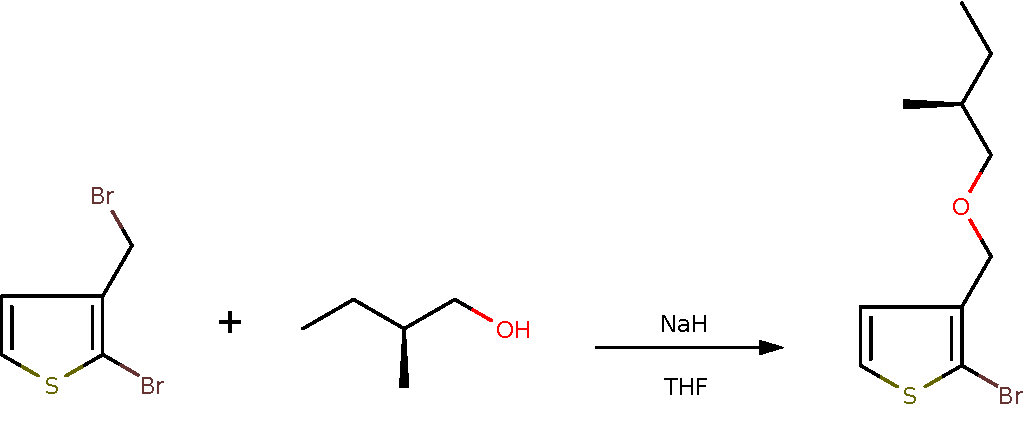
\includegraphics[scale=0.7]
{syn1-eterificazione.pdf}
\caption{Etherification reaction.}
\label{fig:syn1-eterificazione}
\end{SCfigure}

Enantiopure (S)-2-methyl-1-butanol and scalemic 2-methyl-1-butanol alcohols were deprotonated in tetrahydrofuran using one equivalent of sodium hydride, then their alkoxides were reacted in a nucleophilic substitution with commercial 
2-bromo-3-(bromo\-methyl)\-thio\-phene giving 2-bromo-3-[(2-methyl\-butyl\-oxy)\-methyl]\-thio\-phene \cmpd+{ig2-9} and 2-bromo-3-[((S)-2-methyl\-butyl\-oxy)\-methyl]\-thio\-phene \cmpd+{ig2-1}. Refer to Section~\ref{sec:ig2-9} for complete experimental procedure.\superfootcite{Lee2011} Purity was confirmed by \gls{TLC} and \gls{GCMS}. 
The electronic effect of the oxy\-genated side group on the thio\-phene ring was estimated via computational calculations. Comparing molecular orbital energies of 3-propyl\-thio\-phene with 3-(meth\-oxy\-methyl)\-thio\-phene, the oxy\-gen atom resulted to have an electron withdrawing effect on the thio\-phenic ring (optimization and energy calculation Gaussian09c01\-/DFT\-/B3LYP\-/cc-pVDZ). This is confirmed by cyclic voltammetry on similar polymers reported in the literature.\superfootcite{Zoombelt2008}

\end{subsection}
\begin{subsection}{Iodination}

\begin{SCfigure}[][tbp]%syn2-iodurazione
\centering
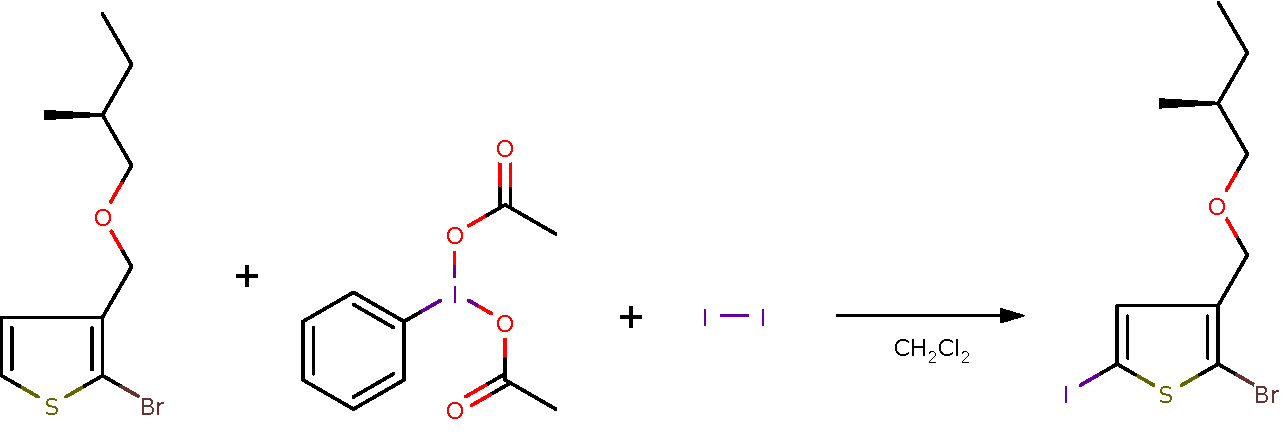
\includegraphics[width=0.95\textwidth]
{syn2-iodurazione.pdf}
\caption{Regioselective iodination.}
\label{fig:syn2-iodurazione}
\end{SCfigure}
The chosen polymerization strategy requires a iodinated-brominated thio\-phene monomer, thus the previously synthesized ether was iodinated selectively in position 5. 

In a dichloromethane solution of 2-bromo-3-[(2-methyl\-butyl\-oxy)\-methyl]\-thio\-phene \cmpd+{ig2-9} or 2-bromo-3-[((S)-2-methyl\-butyl\-oxy)\-methyl]\-thio\-phene \cmpd+{ig2-1}, iodine and iodo\-benzene di\-acetate were added to obtain the desired monomer 2-bromo-5-iodo-3-[((S)-2-methyl\-butyl\-oxy)\-methyl]\-thio\-phene \cmpd+{ig2-10} or 2-bromo-5-iodo-3-[((S)-2-methyl\-butyl\-oxy)\-methyl]\-thio\-phene \cmpd+{ig2-2}, as indicated in Figure~\ref{fig:syn2-iodurazione}. 
Refer to Section~\ref{sec:ig2-10} for complete experimental procedure.\superfootcite{Locke2010} The structure was verified by {\HNMR}, {\CNMR} and \gls{FTIR} characterization. Partial confirmation of {\HNMR} and {\CNMR} data can be found in \citeauthor*{Locke2010}\superfootcite{Locke2010} looking for molecule S6. Purity was confirmed by \gls{TLC} and \gls{GCMS}.

The quantities of iodine and iodo\-benzene di\-acetate are crucial to obtain only the mono\-iodinated product. 
The presence of a iodine atom allows us to activate selectively the desired position without competition from the bromine atom, as we'll see in the next section. 
\end{subsection}
\begin{subsection}{Metalation Reaction}
\label{sec:monomero-regioselettivita}

\begin{SCfigure}[][tbp]%syn3-attivazione
\centering
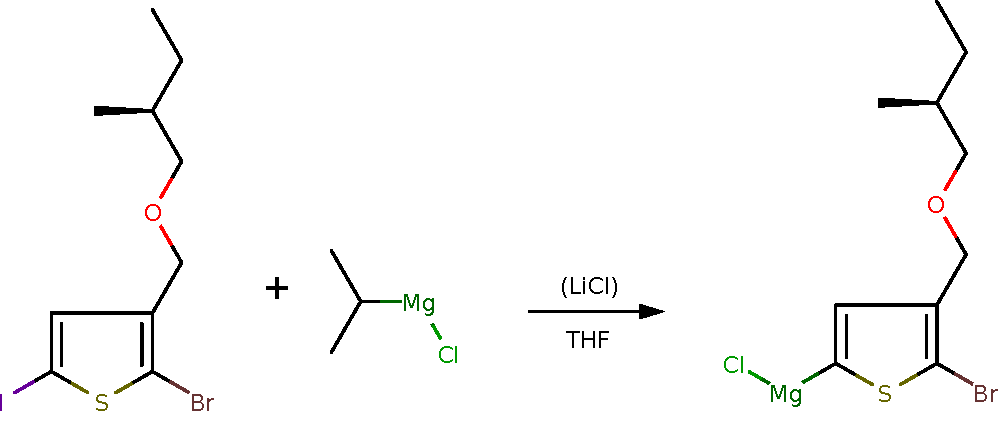
\includegraphics[scale=0.7]
{syn3-attivazione.pdf}
\caption{Metalation activation reaction.}
\label{fig:syn3-attivazione}
\end{SCfigure}
In order to evaluate the regioselectivity of Grignard metathesis we reacted the monomer \cmpd+{ig2-10} with one equivalent of isopropyl magnesium bromide, both in presence and in absence of lithium chloride, and quenched with a solution of hydrochloric acid. Gas chromatography--mass spectrometry (GCMS) analysis showed a complete and regioselective hydrolysis when no lithium chloride is present.
If \ch{LiCl} is added, the product, after washing and extraction, appears to contain a small quantity of immiscible byproduct. \Gls{GCMS} analysis showed a decrease in regio and chemioselectivity. Chromatograms are reported in appendix.

\end{subsection}
\end{section}
\clearpage
\begin{section}{Polymer Synthesis}
For the polymerization of poly\{3-[((S)-2-methyl\-butyl\-oxy)\-methyl]\-thio\-phene\} \cmpd+{ig2-4} we followed the procedure by \citeauthor*{Miyakoshi2005}\superfootcite{Miyakoshi2005} designed for the polymerization of \gls{P3HT}. 

\begin{figure}[tbp]%syn4-polimerizzazione
\centering
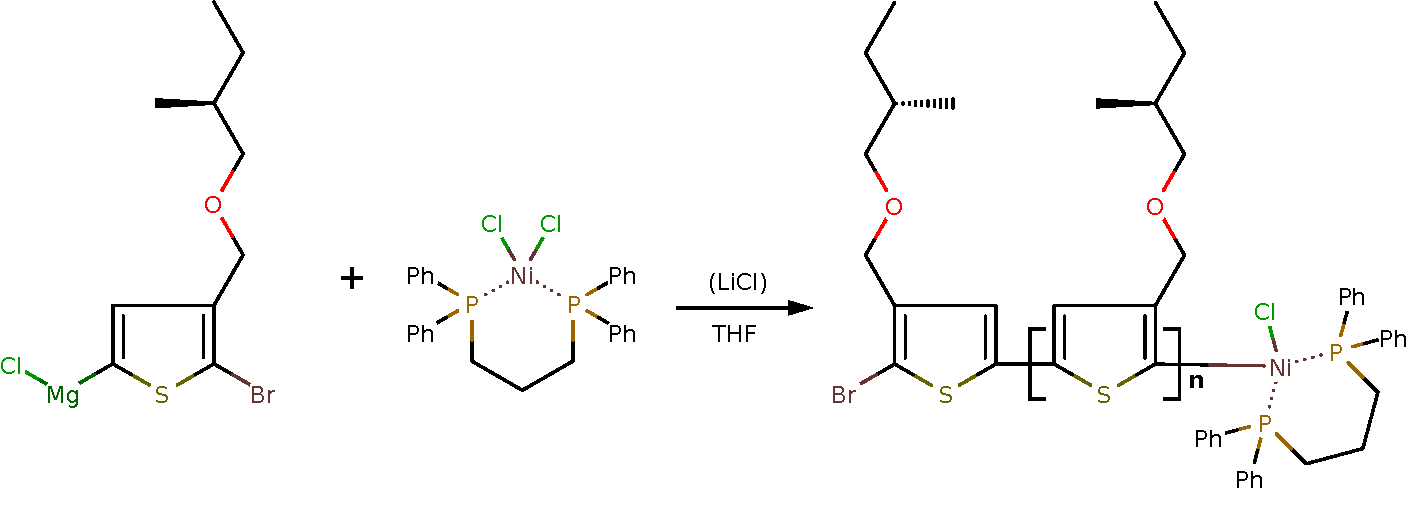
\includegraphics[width=1\textwidth]
{syn4-polimerizzazione.pdf}
\caption{Polymerization method.}
\label{fig:syn4-polimerizzazione}
\end{figure}

Polythio\-phene \cmpd+{ig2-4} was synthesized without addition of lithium chloride. To 2-bromo-5-iodo-3-[((S)-2-methyl\-butyl\-oxy)\-methyl]\-thio\-phene \cmpd+{ig2-2} in dry tetrahydrofuran at \SI{0}{\celsius} under nitrogen atmosphere one equivalent of isopropyl-magnesium chloride was added dropwise. After one hour a suspension of the catalyst \acrfull{nidppp} was poured in reaction mixture and the polymerization remained at room temperature for a day. The reaction was quenched adding \SI{5}{\Molar} hydrochloric acid, resulting in a low weight polymer (see Figure~\ref{fig:ig2-4-ig2-8-sec-chcl3} and Table~\ref{tab:sec}, 
$M_n\approx$~\SI{3.4}{\kg\per\mole} thus $\approx 20$ repeating units).

Afterward we changed the polymerization conditions by following the procedure of 
\citeauthor*{Higashihara2011}\superfootcite{Higashihara2011} designed for the synthesis of poly\-thio\-phene with triethylene glycol side chains to prepare poly\{3-[(2-methyl\-butyl\-oxy)\-methyl]\-thio\-phene\} \cmpd+{ig2-15} and poly\{3-[((S)-2-methyl\-butyl\-oxy)\-methyl]\-thio\-phene\} (\cmpd+{ig2-8}, same repeating unit of \cmpd+{ig2-4}). This procedure is the most common one for monomers bearing hydrophilic oxyethylene side chains,\superfootcite{VanBeek2005}\superfootcite{Hammer2011}\superfootcite{Ohshimizu2008}\superfootcite{Zoombelt2008}\superfootcite{McCullough1993} but procedures with different phosphine ligand are also reported.\superfootcite{Adachi2006}\superfootcite{Yokozawa2008} 
Polymers \cmpd+{ig2-15} and \cmpd+{ig2-8} were synthesized starting respectively from 2-bromo-5-iodo-3-[(2-methyl\-butyl\-oxy)\-methyl]\-thio\-phene \cmpd+{ig2-10} and 2-bromo-5-iodo-3-[((S)-2-methyl\-butyl\-oxy)\-methyl]\-thio\-phene \cmpd+{ig2-2} in presence of lithium chloride. These syntheses resulted in medium weight polymers (see Figure~\ref{fig:ig2-4-ig2-8-sec-chcl3} and Table~\ref{tab:sec}, $M_n\approx$~\SI{10}{\kg\per\mole}, $\approx 50$ repeating units) thus \gls{NMR} signals from initial \textit{tail-to-tail} dyad and from terminations should be negligible if compared with main peaks. 
\cmpd+{ig2-15} and \cmpd+{ig2-8} were carefully purified via various Soxhlet extractions in order to remove catalyst and possible oligomer impurities (see experimental procedure at page~\pageref{sec:ig2-15}).

\begin{subsection}{Regioregularity}
\label{sec:regioregolarita}

As shown in Figure~\ref{fig:triadi} a thio\-phenic unit can be in four different environments, each giving different \gls{NMR} signals. In a regioregular \textit{head-to-tail} poly\-thio\-phene, every backbone ring is in the same environment. Instead a regiorandom polymer would give rise to four different singlets for aromatic protons.\superfootcite{Jeffries-El2005}\superfootcite{Chen1995}\superfootcite{Chen1992}\superfootcite{Zoombelt2008}\superfootcite{Maior1990}\superfootcite{McCullough1993c}

\begin{SCfigure}[][tbp]%ig2-15-nmr-h
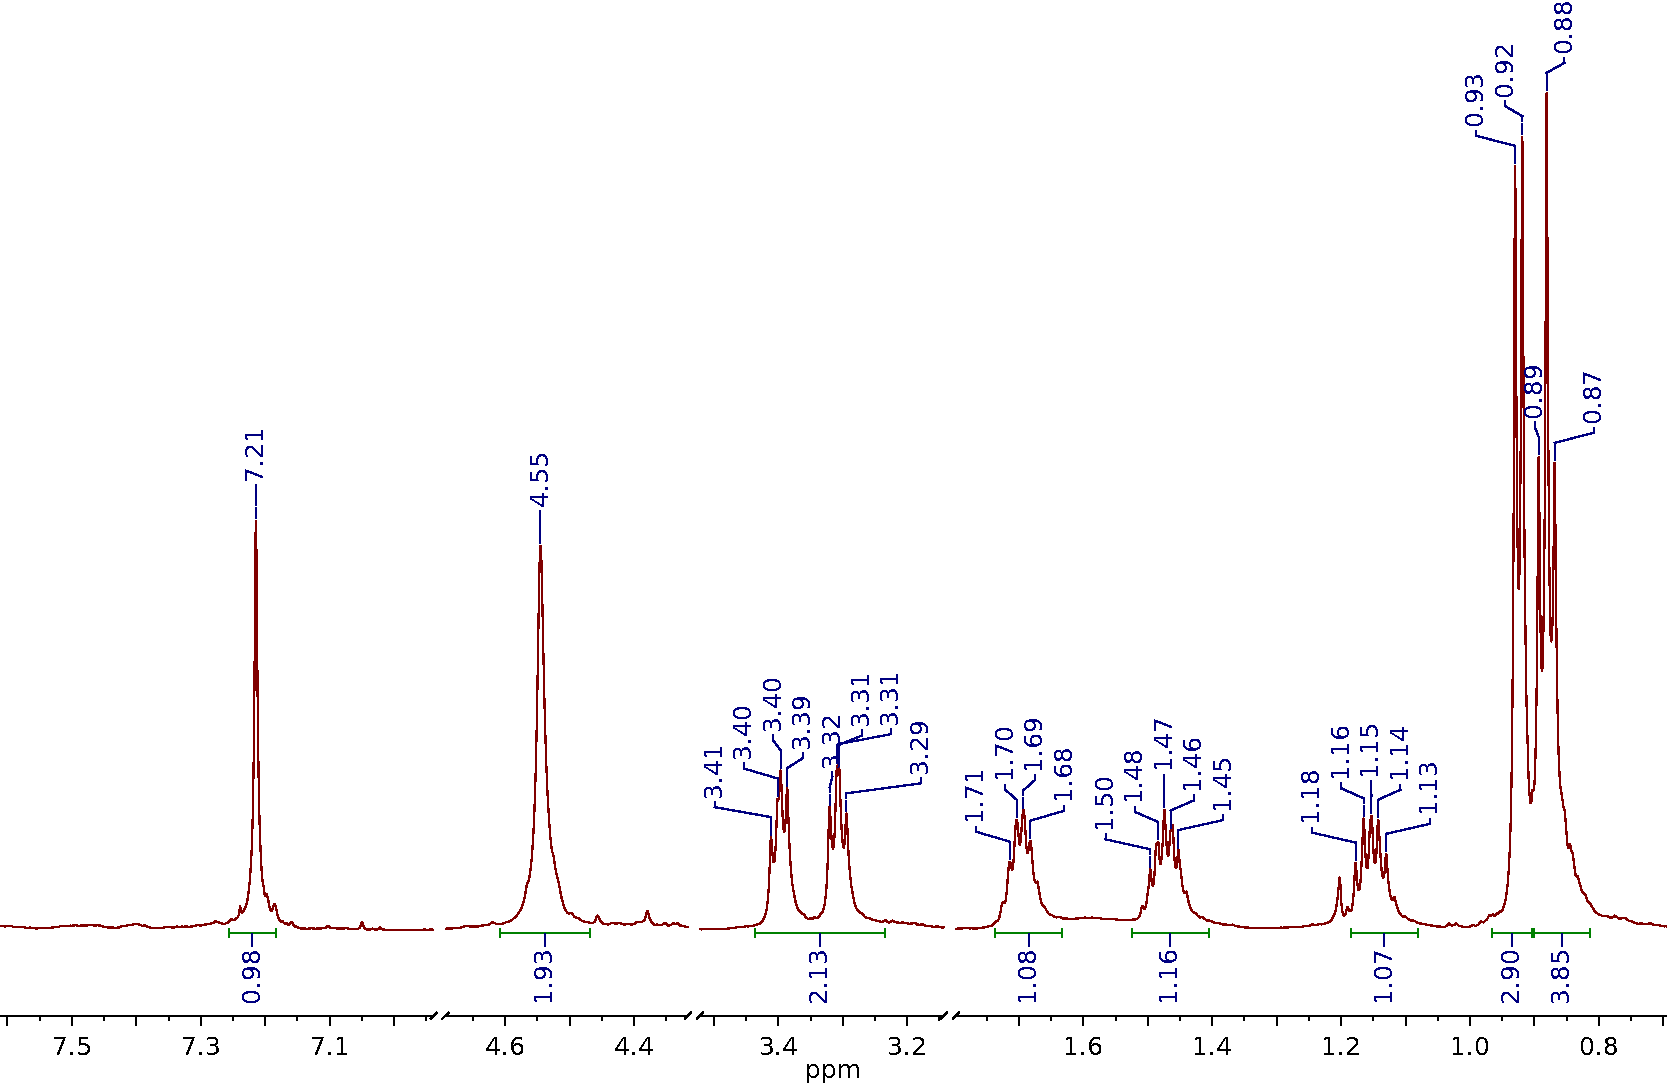
\includegraphics[width=0.9\textwidth]{ig2-15-nmr-h.pdf}
\caption[{\HNMR} of polymer \cmpd+{ig2-15}.]{{\HNMR} (\SI{600}{\MHz}) of polymer \cmpd+{ig2-15} in \gls{TCE}-d2.}
\label{fig:ig2-15-nmr-h}
\end{SCfigure}

\begin{figure}[tbp]%regioregolarita-nmr
\parbox[b]{0.47\linewidth}{
\begin{subfigure}[b]{0.47\textwidth}
\parbox[b]{0\linewidth}{\subcaption{}\label{fig:regioregolarita-nmr-ig2-4}}
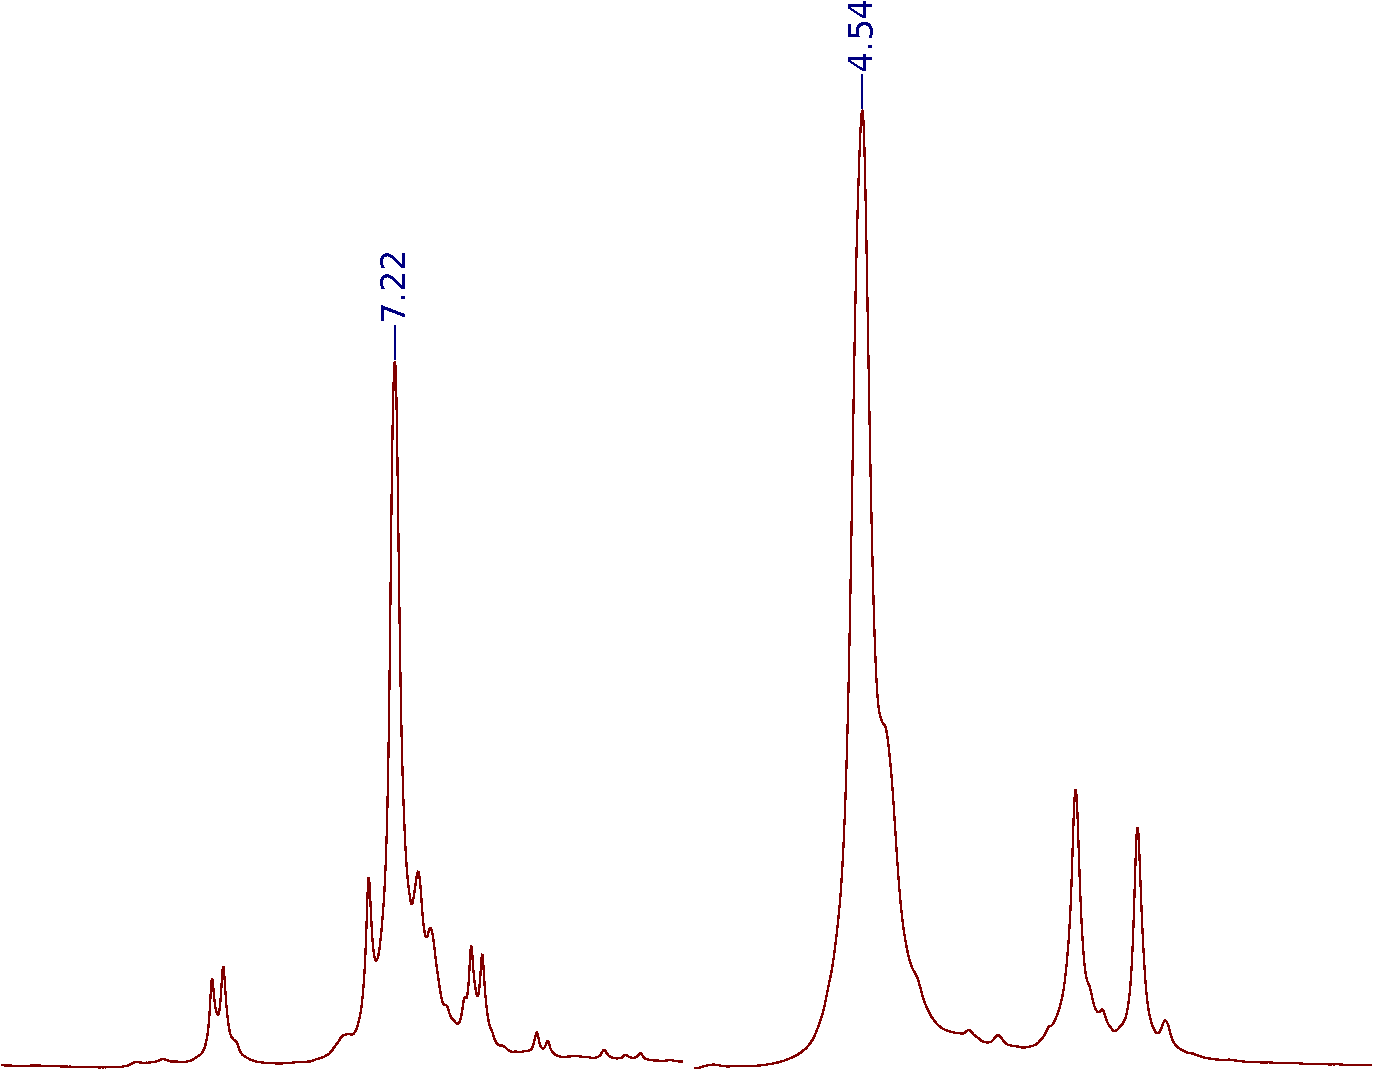
\includegraphics[width=1\textwidth]{regioregolarita-nmr-ig2-4.pdf}
\end{subfigure}}
\qquad
\parbox[b]{0.47\linewidth}{
\begin{subfigure}[b]{0.47\textwidth}
\parbox[b]{0\linewidth}{\subcaption{}\label{fig:regioregolarita-nmr-ig2-4-c}}
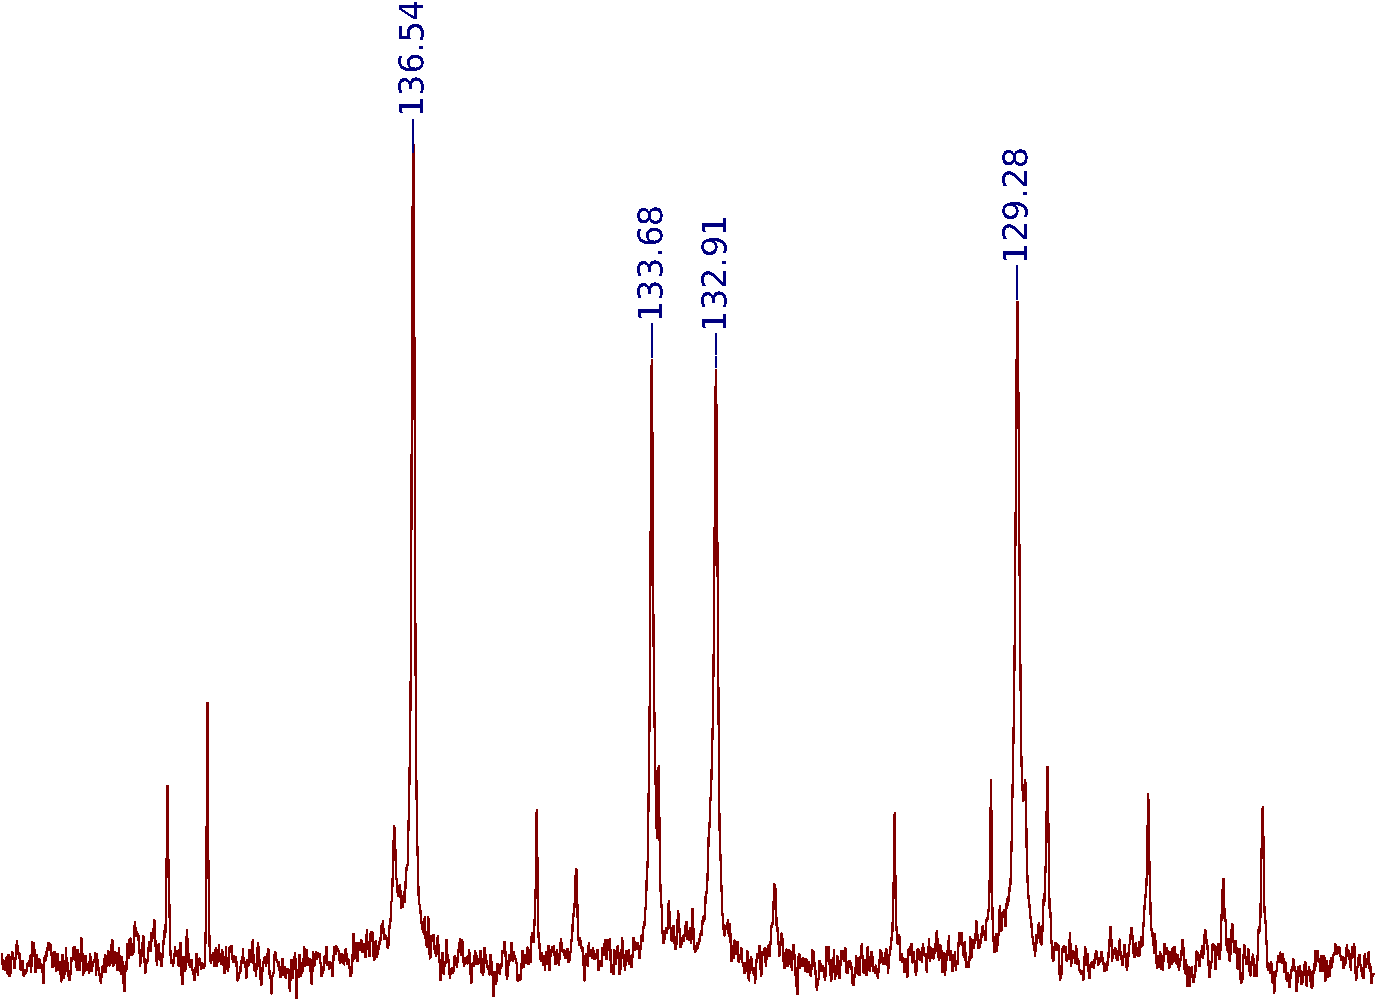
\includegraphics[width=1\textwidth]{regioregolarita-nmr-ig2-4-c.pdf}
\end{subfigure}
}

\parbox[b]{0.47\linewidth}{
\begin{subfigure}[b]{0.47\textwidth}
\parbox[b]{0\linewidth}{\subcaption{}\label{fig:regioregolarita-nmr-ig2-15}}
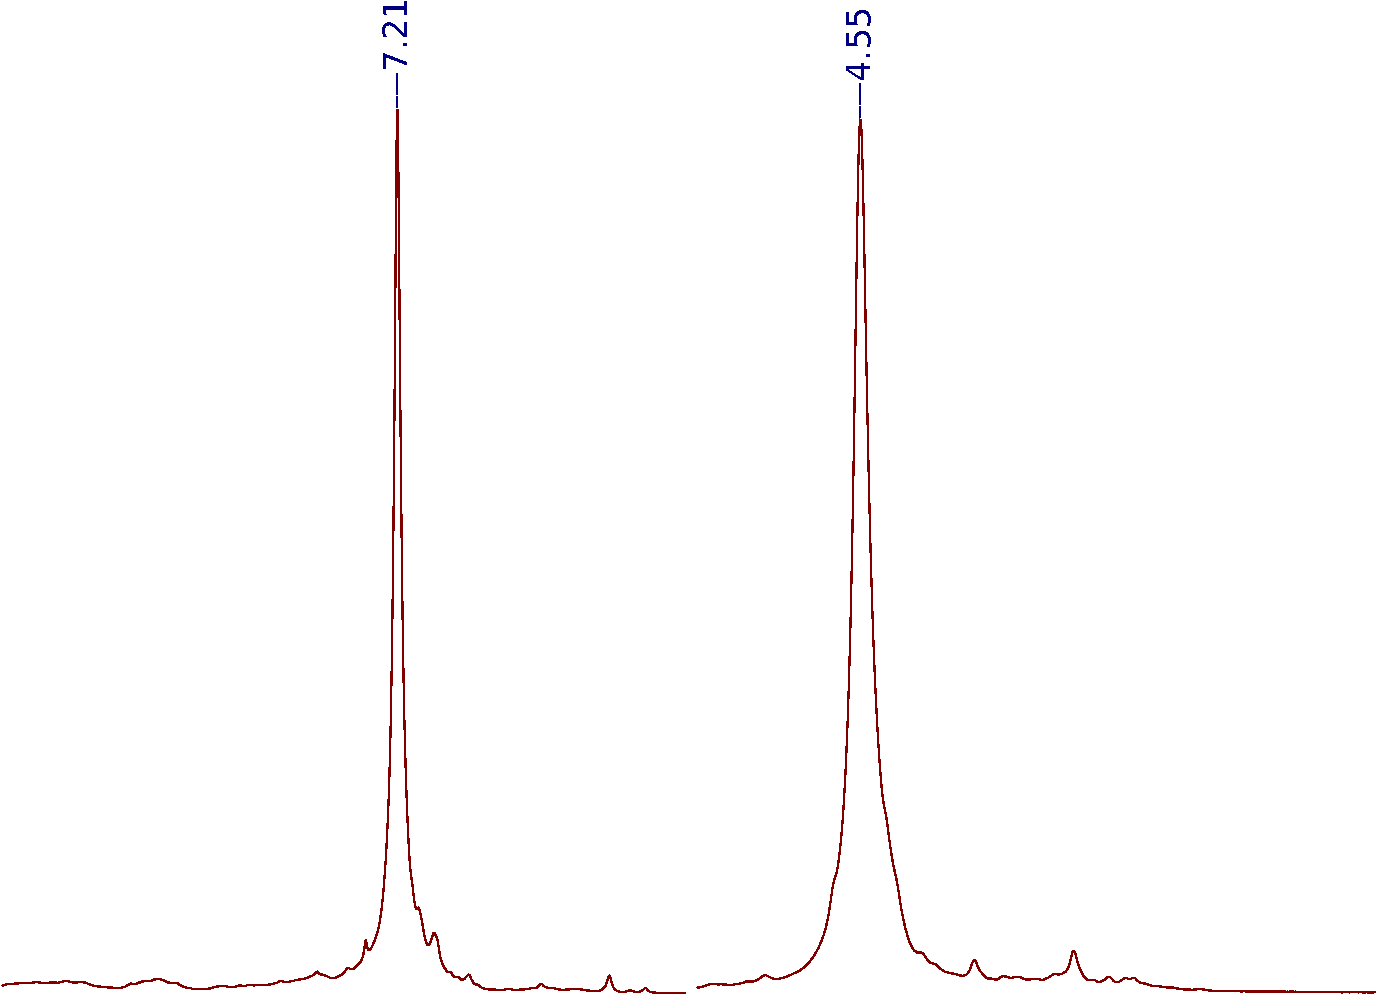
\includegraphics[width=1\textwidth]{regioregolarita-nmr-ig2-15.pdf}
\end{subfigure}}
\qquad
\parbox[b]{0.47\linewidth}{
\begin{subfigure}[b]{0.47\textwidth}
\parbox[b]{0\linewidth}{\subcaption{}\label{fig:regioregolarita-nmr-ig2-15-c}}
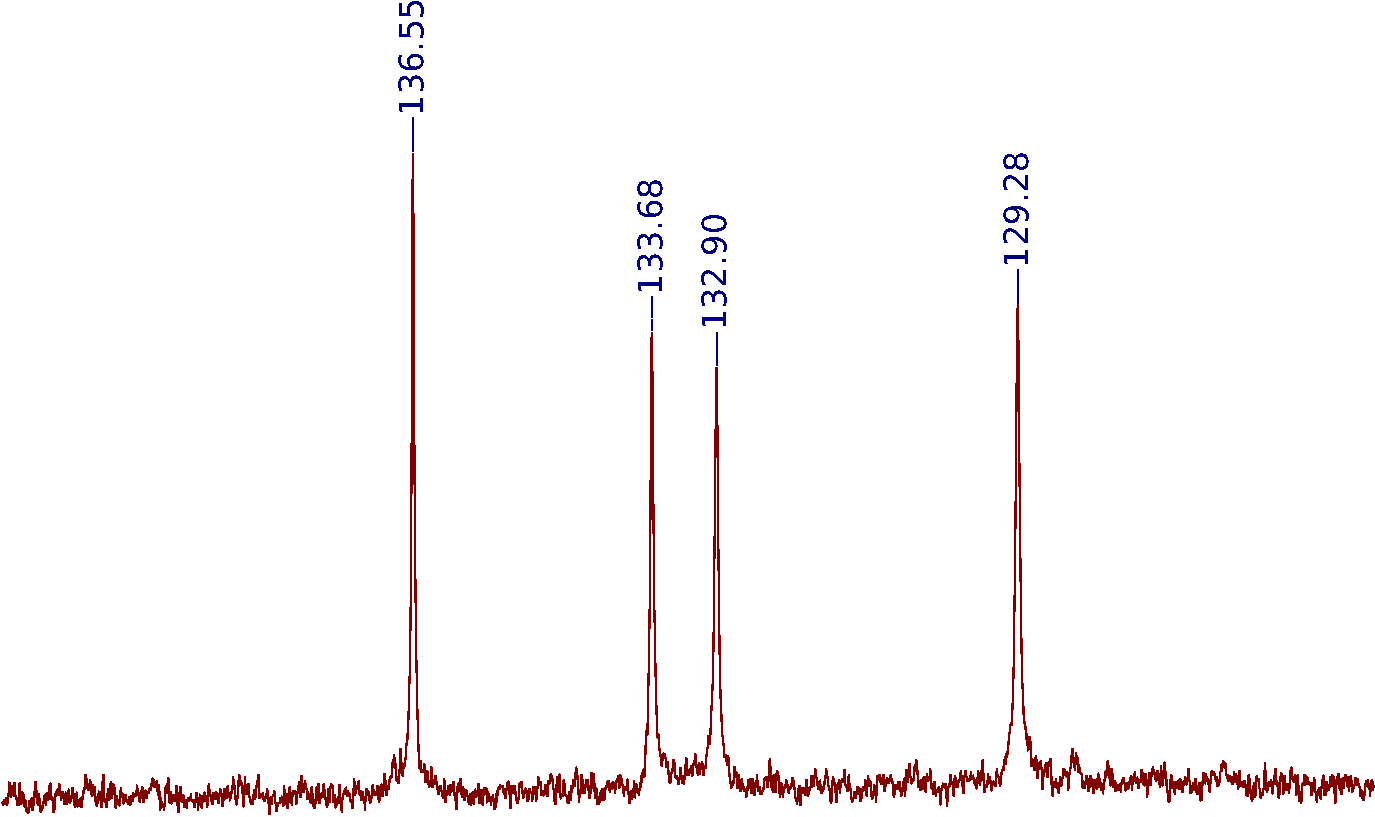
\includegraphics[width=1\textwidth]{regioregolarita-nmr-ig2-15-c.pdf}
\end{subfigure}
}

\parbox[b]{0.47\linewidth}{
\begin{subfigure}[b]{0.47\textwidth}
\parbox[b]{0\linewidth}{\subcaption{\vspace{15pt}}\label{fig:regioregolarita-nmr-ig2-8}}
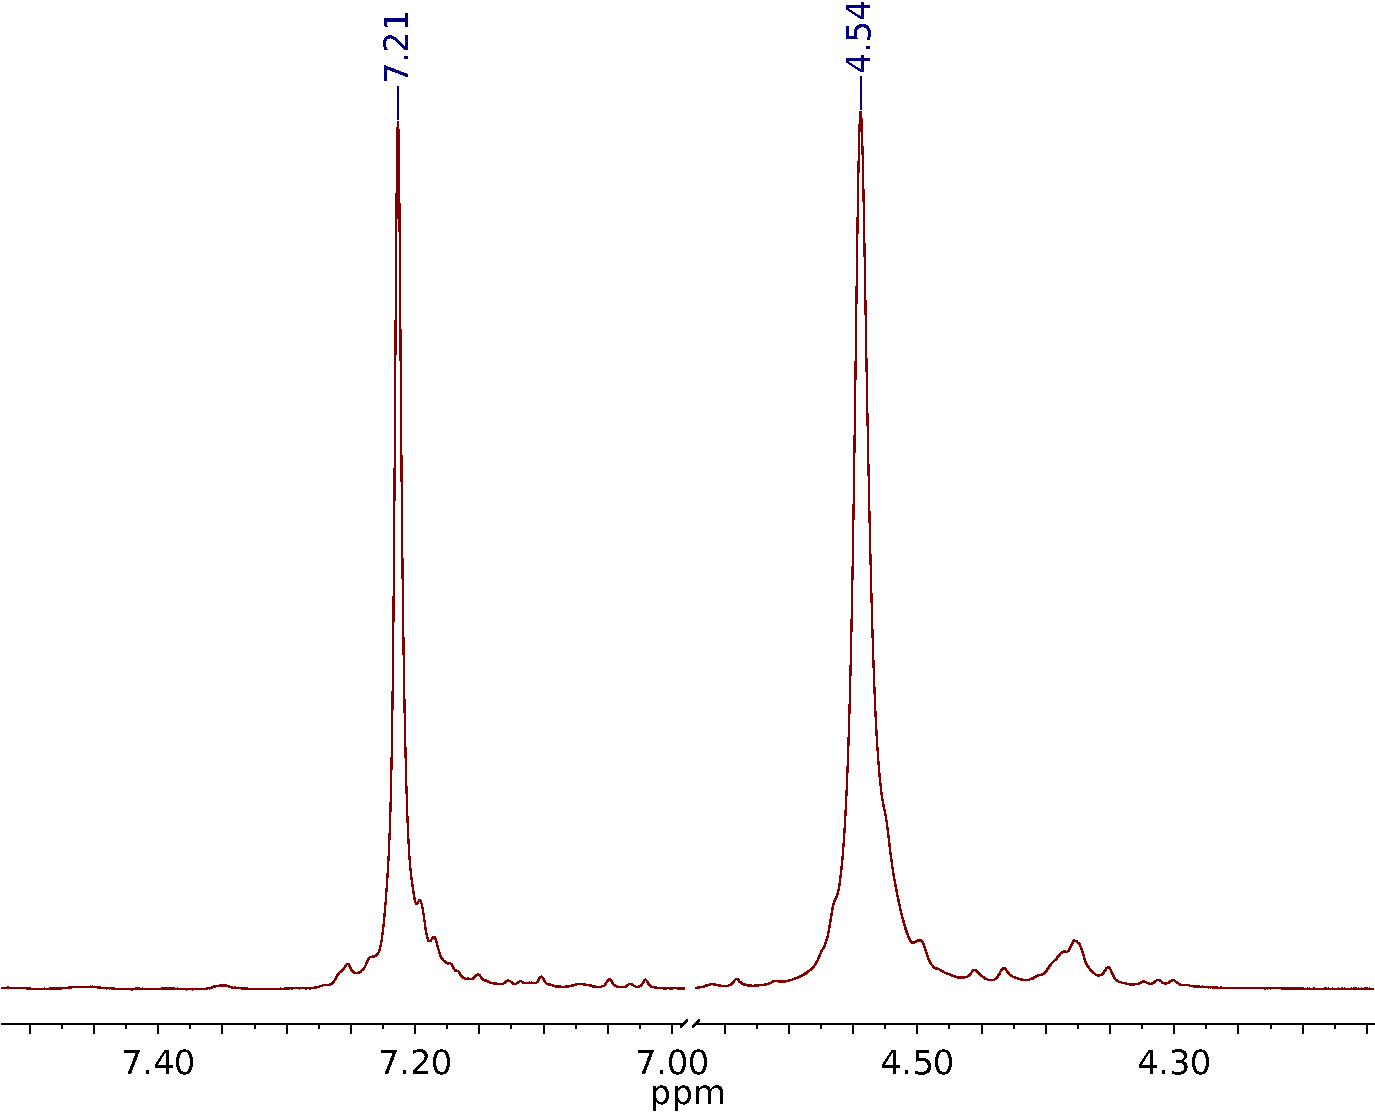
\includegraphics[width=1\textwidth]{regioregolarita-nmr-ig2-8.pdf}
\end{subfigure}}
\qquad
\parbox[b]{0.47\linewidth}{
\begin{subfigure}[b]{0.47\textwidth}
\parbox[b]{0\linewidth}{\subcaption{\vspace{15pt}}\label{fig:regioregolarita-nmr-ig2-8-c}}
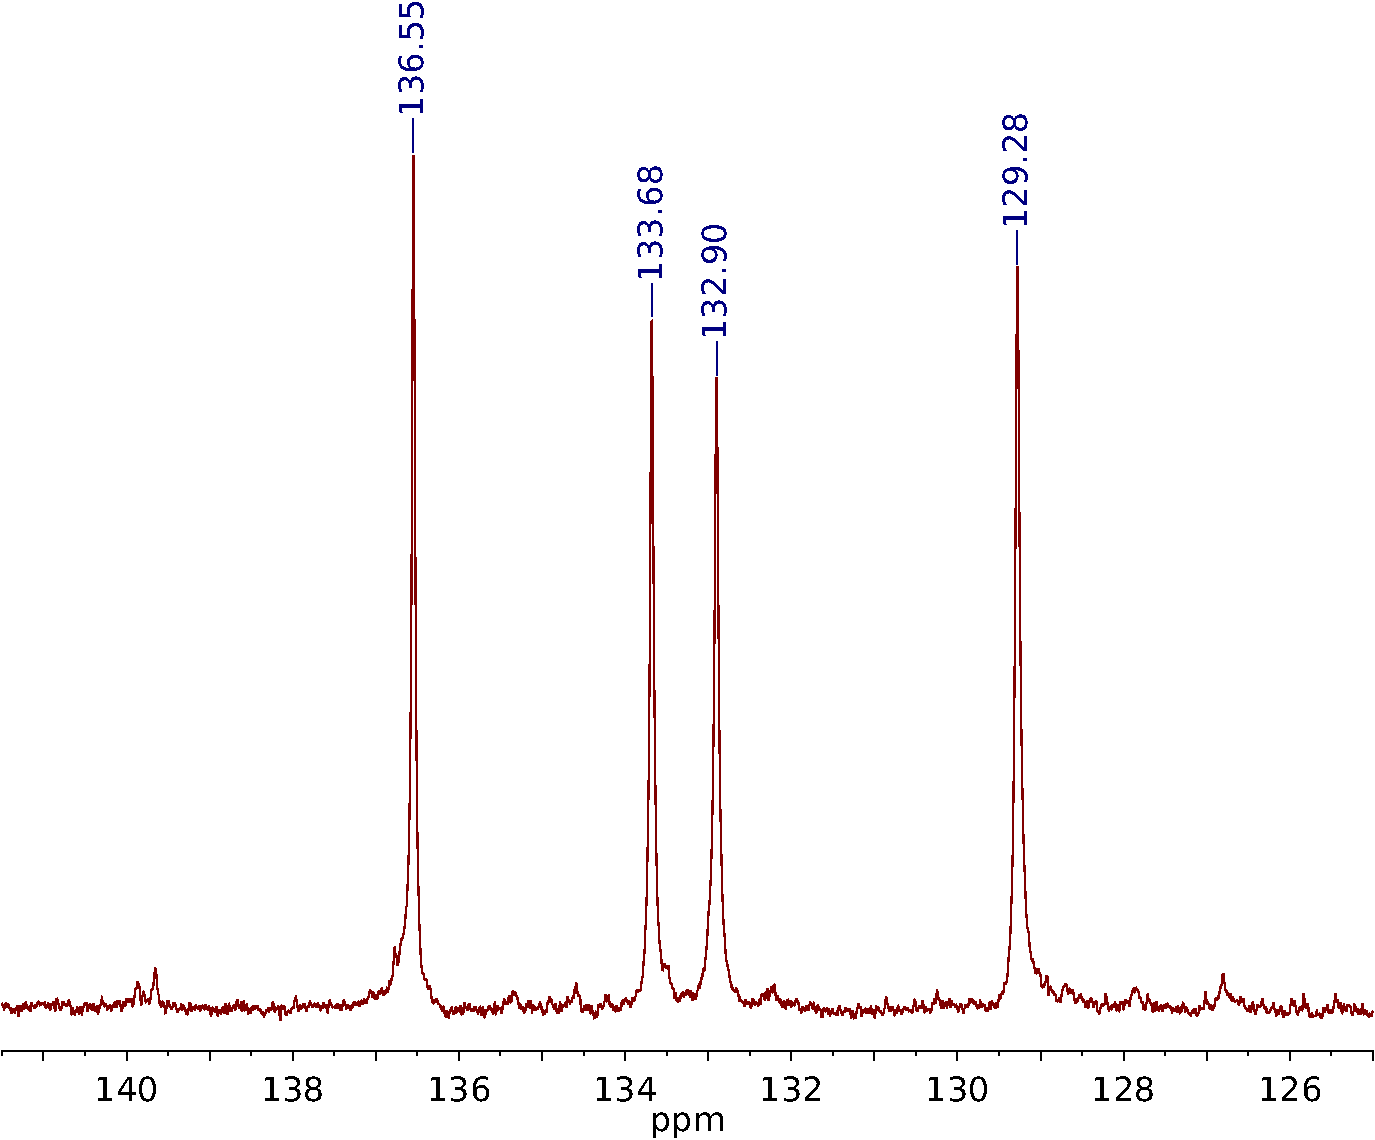
\includegraphics[width=1\textwidth]{regioregolarita-nmr-ig2-8-c.pdf}
\end{subfigure}
}

\caption[Part of {\HNMR} and {\CNMR} spectra in d2-TCE.]{Part of {\HNMR} and {\CNMR} spectra in d2-\gls{TCE}. 
(\subref{fig:regioregolarita-nmr-ig2-4}) and (\subref{fig:regioregolarita-nmr-ig2-4-c}) spectra of low weight polymer \cmpd+{ig2-4}; (\subref{fig:regioregolarita-nmr-ig2-15}) and (\subref{fig:regioregolarita-nmr-ig2-15-c}) spectra of polymer \cmpd+{ig2-15}; (\subref{fig:regioregolarita-nmr-ig2-8}) and (\subref{fig:regioregolarita-nmr-ig2-8-c}) spectra of polymer \cmpd+{ig2-8}.}\label{fig:regioregolarita-nmr}
\end{figure}

{\HNMR} and {\CNMR} spectra of \cmpd+{ig2-4} show many secondary peaks (see Figures~\ref{fig:regioregolarita-nmr-ig2-4} and \ref{fig:regioregolarita-nmr-ig2-4-c}), some of these peaks will be assigned to the end groups of the polymer, see Section~\ref{sec:sintesi-terminazione}. 

{\HNMR} spectra from polymers \cmpd+{ig2-15} and \cmpd+{ig2-8} (see Figures~\ref{fig:regioregolarita-nmr-ig2-15}, \ref{fig:regioregolarita-nmr-ig2-8}, \ref{fig:ig2-15-nmr-h} and appendix) show only a singlet for aromatic hydrogen at \SI{7.21}{\ppm}.

In the region of aliphatic protons in {\HNMR} spectrum from \cmpd+{ig2-15} (see Figures~\ref{fig:regioregolarita-nmr-ig2-15} and \ref{fig:ig2-15-nmr-h}) we can see only main peaks while in {\HNMR} spectrum from \cmpd+{ig2-8} (see Figures~\ref{fig:regioregolarita-nmr-ig2-8} and appendix%
) there are small secondary peaks indicating a lower molecular weight or a higher percent of hydrogen substituted chain ends. For a full assignment of {\HNMR} and {\CNMR} signals refer to Table~\ref{tab:ig2-4-nmr2d}.
{\CNMR} spectra of these polymers (see Figures~\ref{fig:regioregolarita-nmr-ig2-15-c} and \ref{fig:regioregolarita-nmr-ig2-8-c}, complete spectra in appendix) show only four resonances in the aromatic region, corresponding to the four carbons of the thio\-phene ring repeating unit with \textit{head-to-tail} orientation,\superfootcite{Maior1990}\superfootcite{McCullough1993} thus the regioregularity seems complete.\superfootcite{McCullough1993c} 
Some very small peaks from impurities, noticeable in Figure~\ref{fig:regioregolarita-nmr-ig2-8-c}, are present also in Figure~\ref{fig:regioregolarita-nmr-ig2-4-c} (corresponding to peaks reported in Table~\ref{tab:ig2-4-nmr2d-10}).
\end{subsection}
\begin{subsection}{Polydispersity and Molecular Weight}
\label{sec:weight}

\afterpage{\clearpage
\begin{figure}[tbhp]%ig2-4-ig2-8-sec-chcl3
\centering
\begin{tikzpicture}
\begin{axis}[axis x line=bottom,axis y line=left,xlabel=Slice Log MW,ylabel=dwt/d(logM),width=1\textwidth,height=6cm,cycle list name=linestyles*]
\addplot file {img/spectra/ig2-4-sec-chcl3.txt};
\addlegendentry{\cmpd+{ig2-4}};
\addplot file {img/spectra/ig2-8-sec-chcl3.txt};
\addlegendentry{\cmpd+{ig2-8}};
\end{axis}
\end{tikzpicture}
\caption[SEC chromatograms at \SI{35}{\celsius} in \ch{CHCl3} of polymer \cmpd+{ig2-4} and \cmpd+{ig2-8}.]{SEC chromatograms at \SI{35}{\celsius} in \ch{CHCl3} of polymer \cmpd+{ig2-4}: $M_{peak}=$~\SI{3.9}{\kg\per\mole}, $M_n=$~\SI{3.4}{\kg\per\mole}, $M_w=$~\SI{4.4}{\kg\per\mole}, $M_z=$~\SI{5.7}{\kg\per\mole}, $M_{z+1}=$~\SI{7.1}{\kg\per\mole}, $M_w/M_n=$~1.32, $M_z/M_w=$~1.29 and of polymer \cmpd+{ig2-8}: $M_{peak}=$~\SI{12.9}{\kg\per\mole}, $M_n=$~\SI{10.6}{\kg\per\mole}, $M_w=$~\SI{14.8}{\kg\per\mole}, $M_z=$~\SI{20.2}{\kg\per\mole}, $M_{z+1}=$~\SI{26.7}{\kg\per\mole}, $M_w/M_n=$~1.39, $M_z/M_w=$~1.37. Conditions for recording both chromatograms were the same.}
\label{fig:ig2-4-ig2-8-sec-chcl3}
\end{figure}
\begin{table}[tbhp]%sec
\centering
\caption[Data from size exclusion chromatograms of polymers \cmpd+{ig2-4}, \cmpd+{ig2-15} and \cmpd+{ig2-8}.]{Data from size exclusion chromatograms of polymers \cmpd+{ig2-4}, \cmpd+{ig2-15} and \cmpd+{ig2-8} in chloroform and ortho-di\-chloro\-benzene (o-\textsmaller{DCB}).}\label{tab:sec}
\begin{tabular}{c|c|c|c|c}
\toprule
Polymer & Method & $M_n$ (\SI{}{\g\per\mol}) & $M_w$ (\SI{}{\g\per\mol}) & $M_w/M_n$\\\cmidrule{1-5}
\cmpd+{ig2-4}\textsuperscript{a} & \ch{CHCl3}, \SI{35}{\celsius} & 3359 & 4420 & 1.32 \\
\cmpd+{ig2-8}\textsuperscript{a} &\ch{CHCl3}, \SI{35}{\celsius} & 10550 & 14873 & 1.41 \\
\cmpd+{ig2-8}\textsuperscript{a} & o-\textsmaller{DCB}, \SI{145}{\celsius} & 7556 & 12511 & 1.66 \\
\cmpd+{ig2-15}\textsuperscript{a} & o-\textsmaller{DCB}, \SI{145}{\celsius} & 7700 & 13351 & 1.73 \\
\cmpd+{ig2-4}\textsuperscript{b} & \acrshort{THF}, \SI{35}{\celsius} & 3590 & 4620 & 1.29 \\
\cmpd+{ig2-8}\textsuperscript{b} & \acrshort{THF}, \SI{35}{\celsius} & 10825 & 14335 & 1.32 \\
\cmpd+{ig2-15}\textsuperscript{b} & \acrshort{THF}, \SI{35}{\celsius} & 14800 & 20130 & 1.36 \\
\bottomrule
\end{tabular}
\smallskip 

{\textsuperscript{a} measured in Milan; \textsuperscript{b} measured in Catania.}
\end{table}
}

It is known that the use of a folded random coil polystyrene as a standard for size exclusion chromatography leads to an overestimation of the polymeric weight of our rigid rod poly\-thio\-phenes.\superfootcite{Wong2012} 

After purification of \cmpd+{ig2-4} the yield was low (maybe due to losses during purification) and the resulting polymer was rather an oligomer ($\mathrm{M_n}\approx$~\SI{3.3}{\kg\per\mole}, corresponding to $\approx18$ repeating units, polydispersity index $M_w/M_n=$~1.32), as seen by \gls{SEC} in Figure~\ref{fig:ig2-4-ig2-8-sec-chcl3}. This shortness could be caused by the presence of an oxy\-gen atom in our side chain. This oligomer was used for \gls{NMR2D} characterization reported in Section~\ref{sec:terminazioni-nmr2d}.

According to its bi\-modal peak in size-exclusion chromatogram reported in Figure~\ref{fig:ig2-4-ig2-8-sec-chcl3}, polymer \cmpd+{ig2-8} contains two families of polymers: the most abundant one with molar mass~\SI{\approx 13}{\kg\per\mole} and the minor one with molar mass~\SI{\approx 27}{\kg\per\mole}. This indicates the presence of a dimerization reaction during the overnight polymerization. 
We can exclude a dimerization during the quenching performed with aqueous hydrochloric acid.\superfootcite{Miyakoshi2004}\superfootcite{Lohwasser2011} Size-exclusion chromatography at \SI{145}{\celsius} in ortho-di\-chloro\-benzene was performed as a check (see Table~\ref{tab:sec}). The resulting polydispersity index (\acrshort{PDI}) measured in chloroform $M_w/M_n = 1.39$ is better than the reported \gls{PDI} $M_w/M_n=1.68$ of a poly\-thio\-phene polymerized with \gls{GRIM}\-/\gls{KCTP} and a very similar side chain.\superfootcite{Zoombelt2008}
Number average molecular weight obtained in our synthesis ($M_n =$~\SI{10.6}{\kg\per\mole}) corresponds to around 58 repeating units and is compatible with the monomer to catalyst feed ratio (45:1) but lower than the molar mass from the reference article ($M_n =$~\SI{16.5}{\kg\per\mole}).\superfootcite{Higashihara2011} 
By the way, the resulting molar mass is higher than $M_n$ of \cmpd+{ig2-4}, we attribute this enhancement to the addition of lithium chloride. The yield in \cmpd+{ig2-8} (estimated from recovered weight after purification) is $\approx 78~\%$. 

Results from \gls{SEC} at room temperature in tetrahydrofuran of polymer \cmpd+{ig2-15} indicate a higher molecular weight than for polymer \cmpd+{ig2-8} and a broader polydispersity, this is in accordance with data obtained from \gls{SEC} characterizations at \SI{145}{\celsius} in ortho-di\-chloro\-benzene (see Table~\ref{tab:sec}). In the chromatograms recorded in \gls{THF} we can see the presence of peaks at higher molecular weight related to aggregated chains, thus confirming the \gls{THF} as a non perfect solvent. 
The yield in \cmpd+{ig2-15} (estimated from recovered weight after purification) is $\approx 61~\%$.

\end{subsection}
\begin{subsection}{Chain Termini}
\label{sec:sintesi-terminazione}

Quenching a living polymerization with \SI{5}{\Molar} aqueous hydrochloric acid should inactivate the catalyst and insert a hydrogen atom in the growing end,\superfootcite{Lohwasser2011} as shown in Figure~\ref{fig:syn5-quenching}.

\afterpage{\clearpage
\begin{SCfigure}%maybe here I should put a [H]
\centering
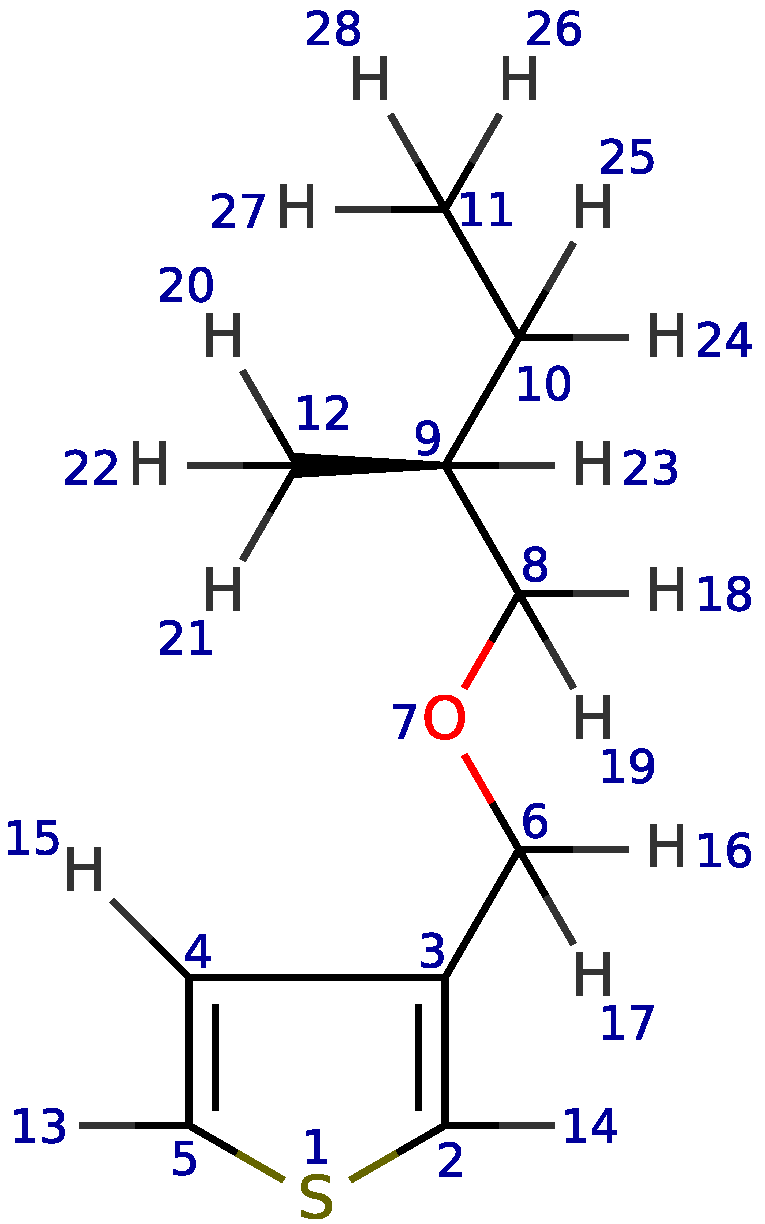
\includegraphics[width=0.2\textwidth]{monomero-numerato.pdf}\caption{Our repeating unit with numbering.}\label{fig:monomero-numerato}
\end{SCfigure}
\begin{table}%maybe here I should put a [H]
\centering
\caption[Groups of {\HNMR} and {\CNMR} signals of \cmpd+{ig2-4} from NMR-2D spectra.]{Groups of {\HNMR} and {\CNMR} signals of \cmpd+{ig2-4} from \gls{NMR2D} spectra. 
}\label{tab:ig2-4-nmr2d}
\begin{subtable}[]{0.49\textwidth}
\centering
\caption{Relative intensity: 1}\label{tab:ig2-4-nmr2d-main}
\begin{tabular}{l|c|l|c}
\toprule
\ch{H} & $\delta$ (ppm) & \ch{C} & $\delta$ (ppm)\\\cmidrule{1-4}
& & {{\ch{C}$_{\textrm 5}$}} & 132.91 \\
& & {{\ch{C}$_{\textrm 2}$}} & 133.68 \\
& & {{\ch{C}$_{\textrm 3}$}} & 136.54 \\
{{\ch{H}$_{\textrm 15}$}} & 7.22 & {{\ch{C}$_{\textrm 4}$}} & 129.28 \\
{{\ch{H}$_{\textrm 16, 17}$}} & 4.54 & {{\ch{C}$_{\textrm 6}$}} & 66.71 \\
{{\ch{H}$_{\textrm 18, 19}$}} & 3.39, 3.31 & {{\ch{C}$_{\textrm 8}$}} & 75.88 \\
{{\ch{H}$_{\textrm 20, 21, 22}$}} & 0.92 & {{\ch{C}$_{\textrm 12}$}} & 16.73 \\
{{\ch{H}$_{\textrm 23}$}} & 1.69 & {{\ch{C}$_{\textrm 9}$}} & 34.86 \\
{{\ch{H}$_{\textrm 24, 25}$}} & 1.15, 1.46 & {{\ch{C}$_{\textrm 10}$}} & 26.25 \\
{{\ch{H}$_{\textrm 26, 27, 28}$}} & 0.88 & {{\ch{C}$_{\textrm 11}$}} & 11.38 \\
\bottomrule
\end{tabular}

\end{subtable}
\begin{subtable}[]{0.49\textwidth}
\centering
\caption{Relative intensity: 0.18}\label{tab:ig2-4-nmr2d-18}
\begin{tabular}{l|c|l|c}
\toprule
\ch{H} & $\delta$ (ppm) & \ch{C} & $\delta$ (ppm)\\\cmidrule{1-4}
{{\ch{H}$_{\textrm 13}$}} & 7.36 $J=5.2$ & {{\ch{C}$_{\textrm 5}$}} & 126.33 \\
& & {{\ch{C}$_{\textrm 2}$}} & 129.60? \\
& & {{\ch{C}$_{\textrm 3}$}} & 139.02?\\
{{\ch{H}$_{\textrm 15}$}} & 7.16 $J=5.1$ & {{\ch{C}$_{\textrm 4}$}} & 128.92 \\
{{\ch{H}$_{\textrm 16, 17}$}} & 4.38 & {{\ch{C}$_{\textrm 6}$}} & 66.41 \\
{{\ch{H}$_{\textrm 18, 19}$}} & 3.16, 3.24 & {{\ch{C}$_{\textrm 8}$}} & 75.72 \\
{{\ch{H}$_{\textrm 20, 21, 22}$}} & 0.85 & {{\ch{C}$_{\textrm 12}$}} & 16.58 \\
{{\ch{H}$_{\textrm 23}$}} & 1.60 & {{\ch{C}$_{\textrm 9}$}} & 34.76 \\
{{\ch{H}$_{\textrm 24, 25}$}} & 1.38, 1.06 & {{\ch{C}$_{\textrm 10}$}} & 26.16 \\
{{\ch{H}$_{\textrm 26, 27, 28}$}} & 0.88 & {{\ch{C}$_{\textrm 11}$}} & 11.32 \\
\bottomrule
\end{tabular}
\end{subtable}
\bigskip

\bigskip

\begin{subtable}[]{0.49\textwidth}
\centering
\caption{Relative intensity: 0.16}\label{tab:ig2-4-nmr2d-16}
\begin{tabular}{l|c|l|c}

\toprule
\ch{H} & $\delta$ (ppm) & \ch{C} & $\delta$ (ppm)\\\cmidrule{1-4}
& & {{\ch{C}$_{\textrm 3, 2}$}} & \tallcell{139.50,\\ 130.76} \\
{{\ch{H}$_{\textrm 15}$}} & 7.24 & {{\ch{C}$_{\textrm 4}$}} & 127.71 \\
{{\ch{H}$_{\textrm 16, 17}$}} & 4.33 & {{\ch{C}$_{\textrm 6}$}} & 66.45 \\
{{\ch{H}$_{\textrm 18, 19}$}} & 3.16, 3.24 & {{\ch{C}$_{\textrm 8}$}} & 75.72 \\
{{\ch{H}$_{\textrm 20, 21, 22}$}} & 0.85 & {{\ch{C}$_{\textrm 12}$}} & 16.58 \\
{{\ch{H}$_{\textrm 23}$}} & 1.60 & {{\ch{C}$_{\textrm 9}$}} & 34.76 \\
{{\ch{H}$_{\textrm 24, 25}$}} & 1.38, 1.06 & {{\ch{C}$_{\textrm 10}$}} & 26.16 \\
{{\ch{H}$_{\textrm 26, 27, 28}$}} & 0.88 & {{\ch{C}$_{\textrm 11}$}} & 11.32 \\
\bottomrule
\end{tabular}
\end{subtable}
\begin{subtable}[]{0.49\textwidth}
\centering
\caption{Relative intensity: $\approx0.10$}\label{tab:ig2-4-nmr2d-10}
\begin{tabular}{l|c|l|c}
\toprule
\ch{H} & $\delta$ (ppm)& \ch{C} & $\delta$ (ppm)\\\cmidrule{1-4}
& & {{\ch{C}$_{\textrm 2, 3, 5}$}} & \tallcell{134.59,\\ 132.20,\\ 136.77?} \\
{{\ch{H}$_{\textrm 15}$}} & 7.19 & {{\ch{C}$_{\textrm 3}$}} & 126.81 \\
{{\ch{H}$_{\textrm 16, 17}$}} & 4.52 & {{\ch{C}$_{\textrm 6}$}} & 66.71\\
\bottomrule
\end{tabular}
\end{subtable}
\end{table}
\clearpage
}

In the aromatic region of {\HNMR} spectrum from \cmpd+{ig2-4} we can see (see Figure~\ref{fig:regioregolarita-nmr-ig2-4}%
) two doublets at 7.15 and \SI{7.35}{\ppm} with scalar coupling $J=$~\SI{5.2}{\Hz}. The presence of two hydrogen atoms on a thio\-phene ring bearing also a side group, implies a hydrogen terminated chain end. An hydrogen in the $\alpha$ position on a thio\-phene ring is expected to be generated by the quenching process of the living chain; this reaction should produce a thio\-phene ring with the 2 and 4 positions (for position numbering refer to Figure~\ref{fig:regioregolarita}) substituted with hydrogen atoms. 
Looking at the amplitude of the $J$-coupling we can verify the relative position of these two protons. 
\label{h-terminale} From the literature on thio\-phene we know that the width of the $J$-coupling for two non vicinal hydrogen atoms in position 2 and 4 is $J\approx$~\SI{1.4}{\Hz}.\superfootcite{Miyakoshi2005} The observed $J$-coupling of \SI{5.2}{\Hz} indicates\superfootcite{Zoombelt2009} the position of hydrogen atoms being vicinal, thus positions 4 and 5. This means that a reversed regioregularity in the ending thio\-phene ring was present. 

\begin{SCfigure}[][tbp]%syn5-quenching
\centering
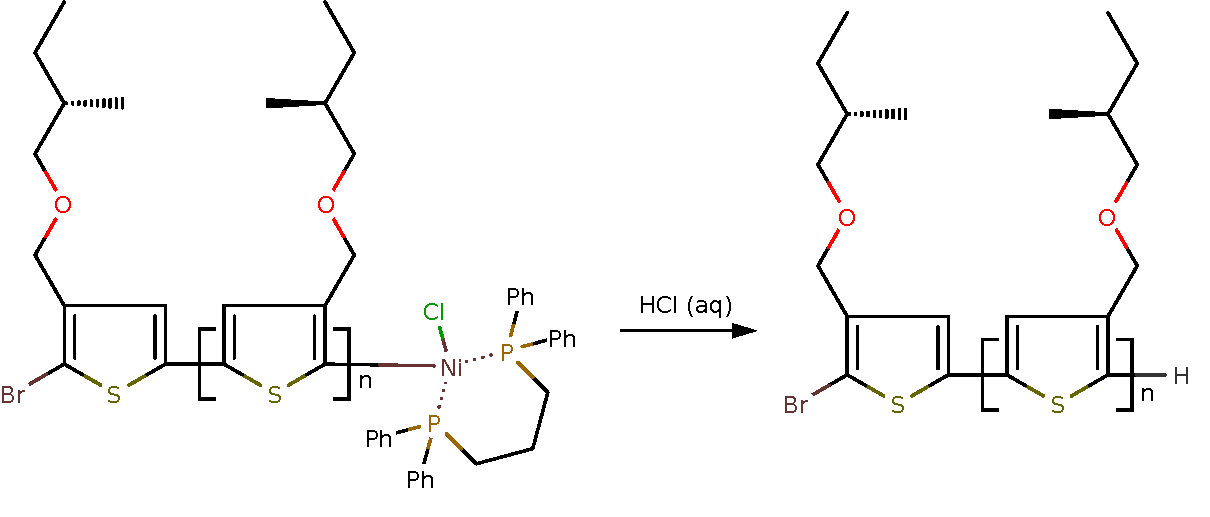
\includegraphics[scale=0.6]
{syn5-quenching.pdf}
\caption{Quenching process.}
\label{fig:syn5-quenching}
\end{SCfigure}

\label{sec:terminazioni-nmr2d}
Analysis of \gls{NMR2D} maps ($^1$\ch{H}-COSY;\nota{\textit{COSY}, two-dimensional correlation spectroscopy.} $^1$\ch{H}-TOCSY;\nota{\textit{TOCSY}, two-dimensional total correlation spectroscopy, also called HOHAHA (homo\-nuclear Hartmann Hahn).} 
$^1$\ch{H},$^{13}$\ch{C}-HSQC;\nota{\textit{HSQC}, hetero\-nuclear single quantum coherence spectroscopy.} $^1$\ch{H},$^{13}$\ch{C}-HMBC\nota{\textit{HMBC}, hetero\-nuclear multiple bond correlation.}) confirms this hypothesis and allows us to distinguish four groups of signals related to four thio\-phenic units present in \cmpd+{ig2-4}. 
The most abundant unit is assigned to \textit{head-to-tail} repetition and is reported in Table~\ref{tab:ig2-4-nmr2d-main}. The previously identified \ch{H} terminated \textit{tail} ending is reported in Table~\ref{tab:ig2-4-nmr2d-18}. Other groups of signals could be due to different terminations or regioregularity defects.

The presence of this \ch{H} terminated \textit{tail} monomer in the chain end could be due to a partial formation of the unintended regioisomer 2-magnesio\-chloro-5-iodo-3-[((S)-2-methyl\-butyl\-oxy)\-methyl]\-thio\-phene (see Section~\ref{sec:monomero-regioselettivita}). This isomer is less reactive\superfootcite{Chen1995}\superfootcite{Loewe2001}\superfootcite{Iovu2005}\superfootcite{Lanni2010}\superfootcite{Lohwasser2011} than 2-bromo-5-magnesio\-chloro-3-[((S)-2-methyl\-butyl\-oxy)\-methyl]\-thio\-phene. 
This \textit{wrong} terminus combined with the low yield make evident that the presence of an oxy\-gen in side chain has a strong negative influence on this living polymerization.

\cmpd+{ig2-15} and \cmpd+{ig2-8} were polymerized with shorter reaction times (\SI{12}{\hour}) and addition of lithium chloride. From {\HNMR} and {\CNMR} characterization these polymers seems very long and regioregular, terminations signals are so weak to make their identification difficult.
In {\CNMR} spectra of \cmpd+{ig2-15} no aromatic carbon signals can be distinguished from the noise except the ones from regioregular repetition (see Figure~\ref{fig:regioregolarita-nmr-ig2-15-c}). In {\CNMR} spectra of \cmpd+{ig2-8} we can recognize also the presence of signals reported for \cmpd+{ig2-4} in Table~\ref{tab:ig2-4-nmr2d-10} (see Figure~\ref{fig:regioregolarita-nmr-ig2-8-c}). 

A reliable quantitative analysis of terminations using \gls{NMR} spectroscopy, both $^1$\ch{H} and $^{13}$\ch{C}, is prevented by the rigid nature of the conjugated polymer backbone that causes an heterogeneous correlation time $\tau_c$. This fact implies a huge experimental work to find the best relaxation time.

Further termination characterization was performed on sample \cmpd+{ig2-8} with \acrfull{MALDI} and \gls{SEC}\-/\gls{MALDI} by the Institute of Chemistry and Technology of Polymers (\textsmaller{ICTP-CNR}, Catania). 
Linear mode mass spectrometry (spectra in appendix) from two different matrices (di\-thranol and $\alpha$-cyano-4-hydr\-oxy\-cinnamic acid) was performed and results are reported in Table~\ref{tab:maldi}. Surprisingly the terminations were completely different from the \ch{H/Br} termination expected from the literature,\superfootcite{Lohwasser2011} this could be related to a quenching of the polymerization 
due to some oxy\-gen or monomers activated with inverse regioselectivity due to the presence of \ch{LiCl}. 
Another hypothesis is that the quenching wasn't effective because of the not so good solubility of the prepared polymer in the polymerization solvent, tetrahydrofuran at room temperature, that could lead to aggregation prior to quenching agent addition thus reducing the quenching efficiency. 

Preliminary results from \gls{SEC}\-/\gls{MALDI} of compound \cmpd+{ig2-8} are reported in Figure~\ref{fig:ig2-8-sec-maldi}.

\begin{table}[tbp]%maldi
\centering
\caption[MALDI-TOF MS results from \cmpd+{ig2-8} in linear mode.]{\Gls{MALDI} results from polymer \cmpd+{ig2-8} in linear mode from dithranol and $\alpha$-cyano-4-hydr\-oxy\-cinnamic acid matrices.}\label{tab:maldi}
\begin{tabular}{c|c|c|c|c}
\toprule
\multirow{2}{*}{terminations}&\multicolumn{2}{c}{\tallcell{relative intensity in\\ dithranol}}&\multicolumn{2}{c}{\tallcell{relative intensity in\\ $\alpha$-cyano-4-hydr\-oxy-\\cinnamic acid}}\\ 
&low mass\textsuperscript{a}&high mass\textsuperscript{b}&low mass\textsuperscript{a}&high mass\textsuperscript{b}\\\cmidrule{1-5}
\ch{H-/-OH}&30&30&30&35\\
\ch{Br-/-I}&70&25&100&40\\
\ch{Br-/-Ni(dppp)Cl}&25&5&30&5\\
\ch{Br-/-OH}&100&50&85&50\\
\ch{Br-/-H}&20&45&30&40\\
\ch{H-/-I}&20&5&40&10\\
\ch{Br-/-Br}&90&100&75&100\\
\ch{Br-/-NiCl}&30&28&40&20\\
\bottomrule
\end{tabular}

\smallskip

\textsuperscript{a} 2.5 $<$ mass \SI{}{\kg\per\mol}$<$ 3.2; \textsuperscript{b} 3.2 $<$ mass \SI{}{\kg\per\mol}
\end{table}

\begin{SCfigure}[][tbp]%ig2-8-sec-maldi
\centering
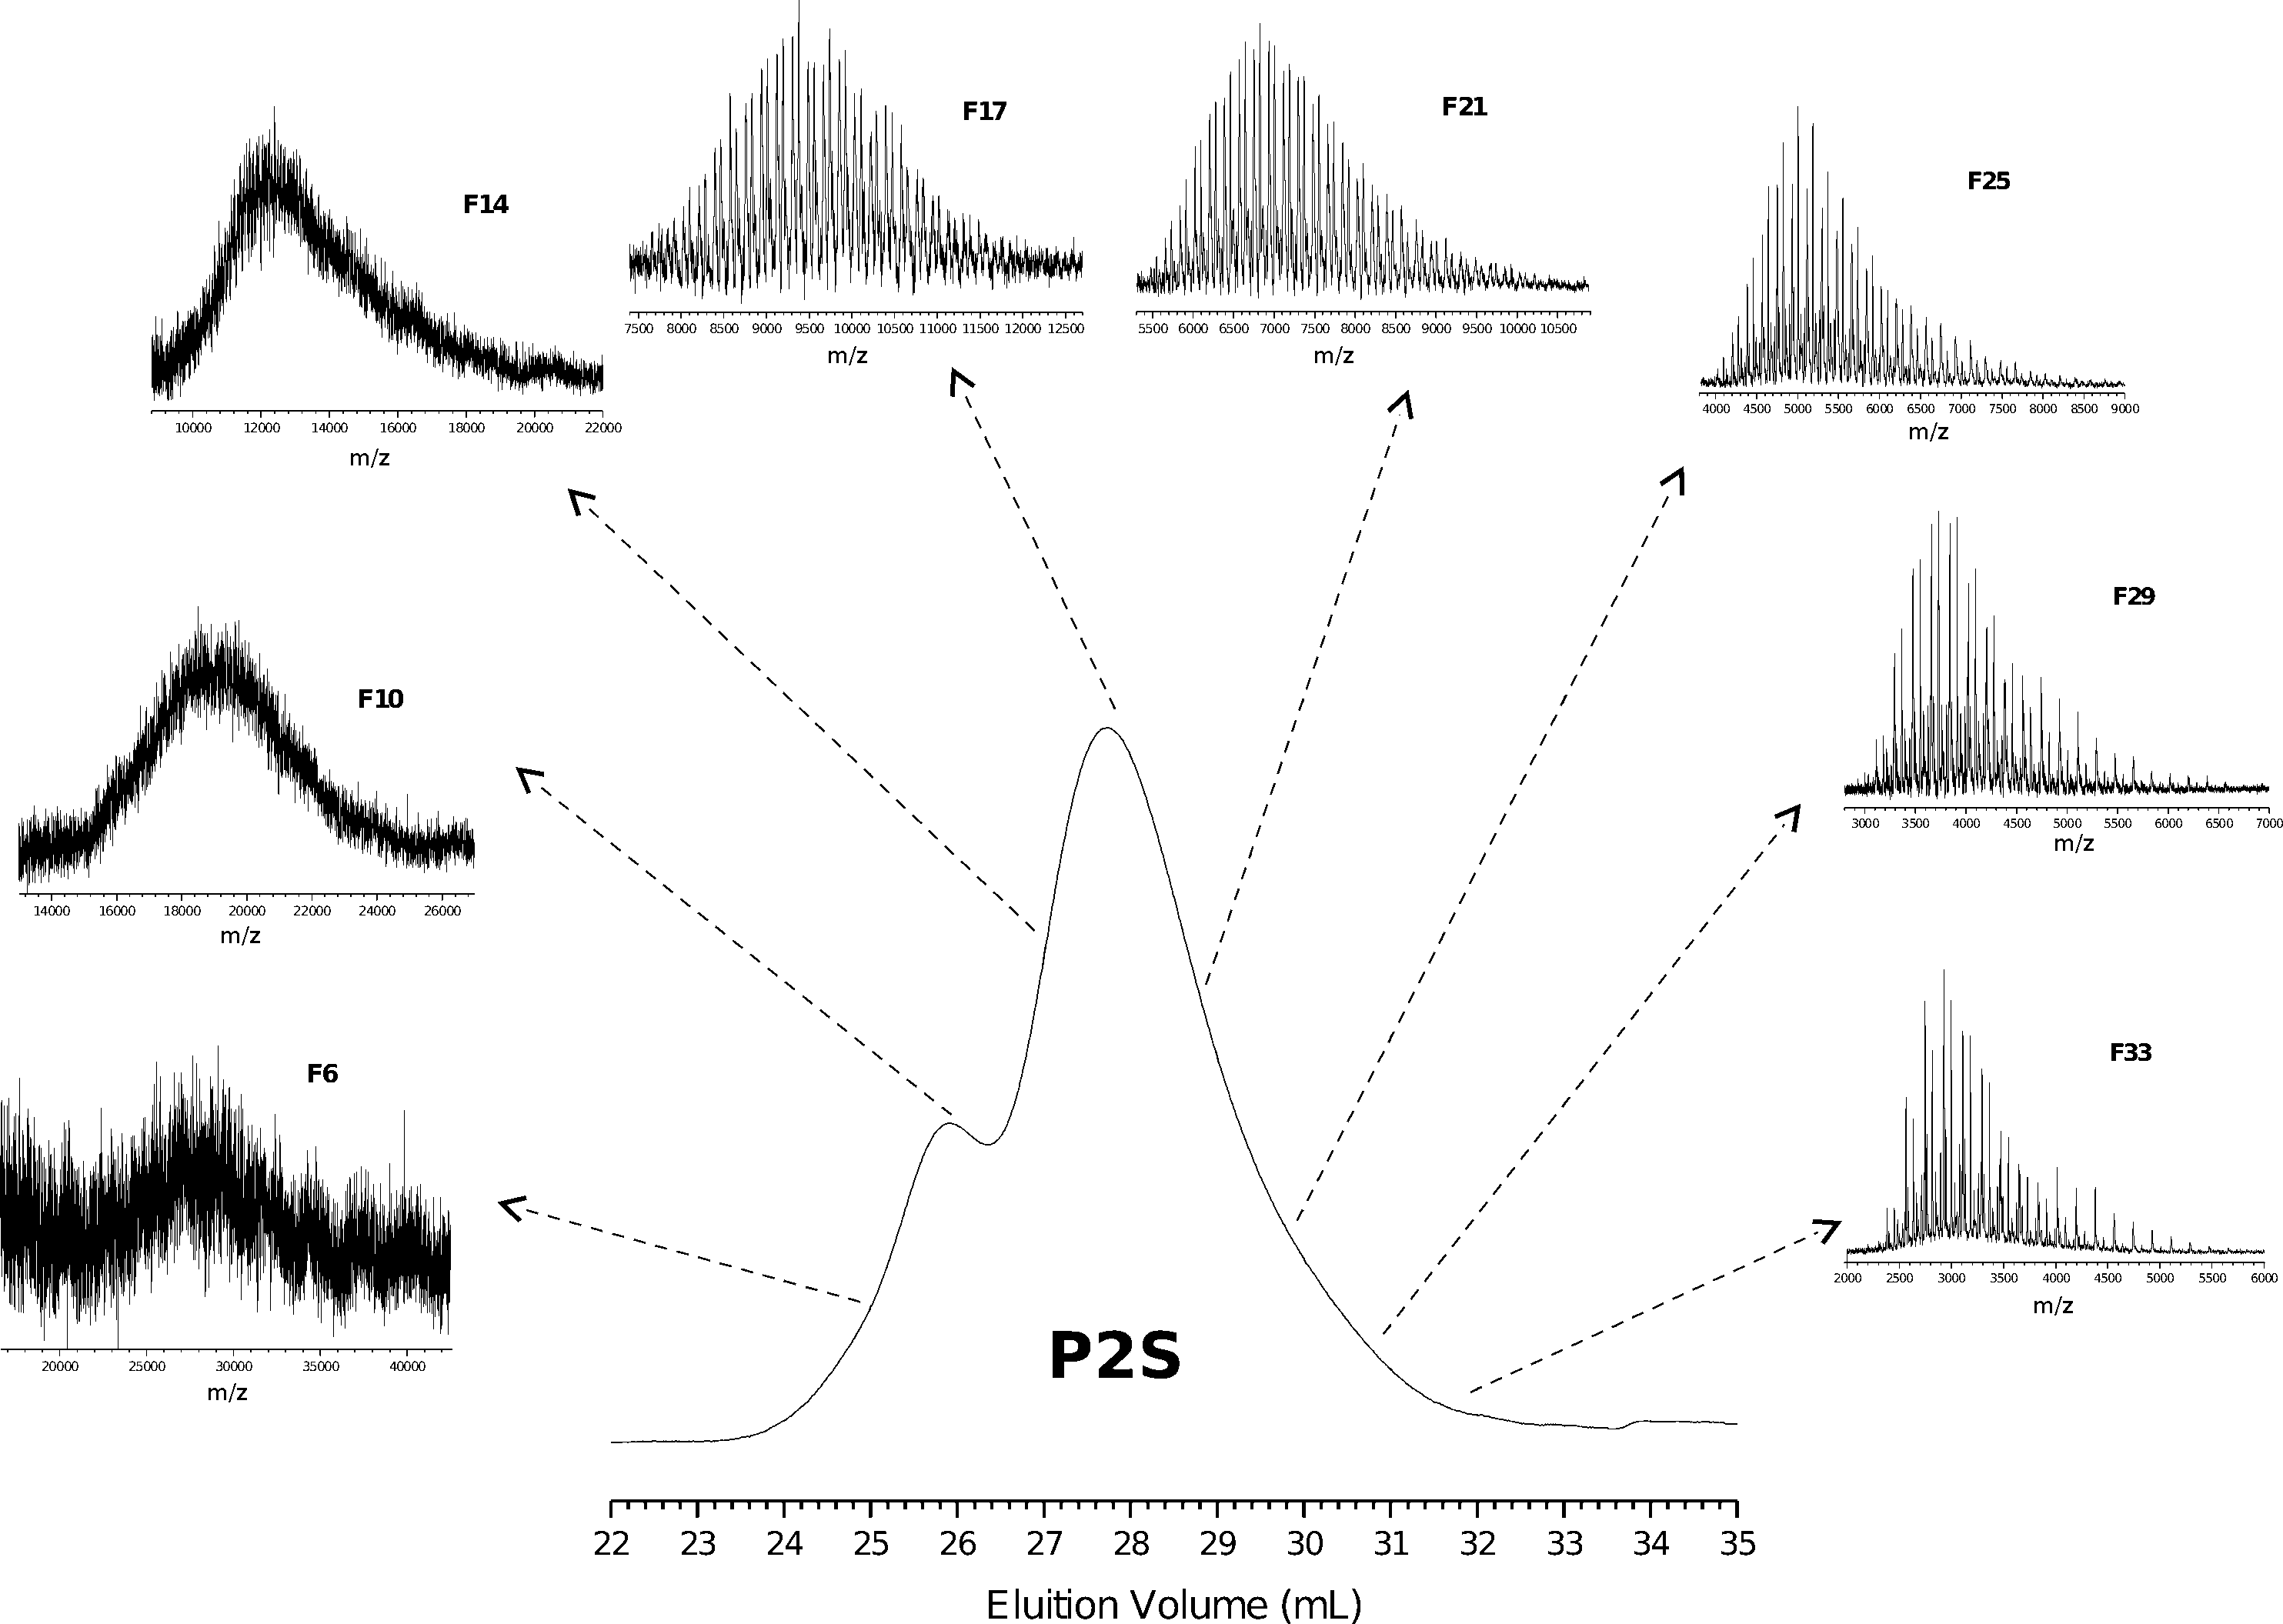
\includegraphics[width=0.8\textwidth]{ig2-8-sec-maldi.png}
\caption[Preliminary results from combined SEC\-/MALDI-TOF MS of \cmpd+{ig2-8}.]{Preliminary results from combined \gls{SEC}\-/\gls{MALDI} of \cmpd+{ig2-8}.}
\label{fig:ig2-8-sec-maldi}
\end{SCfigure}

\end{subsection}
\end{section}
\clearpage
\begin{section}[Optical and Morphological Characterization]{Polymer Optical and Morphological Characterization}
\begin{subsection}{Vibrational Spectroscopy Characterization}
\label{sec:ir}

The main absorption bands observed in the infrared spectra of monomer \cmpd+{ig2-10}, polymers samples and their assignments are listed in Table~\ref{tab:ir}. All of the poly\-thio\-phenes have similar infrared spectra but noticeable differences are evident. Spectra are reported in Figure~\ref{fig:ir}.

The infrared band in the region around \SI{3060}{\per\cm} are related to aromatic \ch{C-H}$_\beta$ ($\beta$ 
is referred to proton in 3 or 4 position) stretching.\superfootcite{Hotta1987} \ch{C-H}$_\alpha$ (\ch{H} in position 2 or 5) 
origins a stretching band around \SI{3105}{\per\cm}, this signal is present in \gls{FTIR} spectrum of \cmpd+{ig2-4} as a shoulder thus confirming the presence of \ch{H}$_\alpha$ as spotted by \gls{NMR} spectra discussed in page~\pageref{h-terminale}.

\textsmaller{IR} bands around 1517 and \SI{1461}{\per\cm} were assigned respectively to the \ch{C=C} antisymmetric stretching vibration and \ch{C=C} symmetric stretching.\superfootcite{Scott1969} 

\noindent
The $I_{antisymm}/I_{symm}$ ratio is reported to increase as the polymerization degree increases thus it is a rough indication of the conjugation length.\superfootcite{Furukawa1987} In our polymers the lowest $I_{a}/I_{s}$ ratio is recorded for \cmpd+{ig2-4} in accordance with his shortest length. 

The \textsmaller{IR} band at \SI{1260}{\per\cm} could be related to the conformation of the poly\-thio\-phene chain.\superfootcite{Winokur1989}

\textsmaller{IR} band in the region 830-\SI{840}{\per\cm} is assigned to aromatic \ch{CH} out-of-plane bending of substituted thio\-phene rings.\superfootcite{Hotta1987} The energy of this band is reported to be indicative of the poly\-thio\-phene regioregularity,\superfootcite{Chen1995}\superfootcite{Caronna1997} in our polymers this energy is comparable with similar regioregular poly\-thio\-phenes.\superfootcite{Ohshimizu2008}

The vibration at \SI{471}{\per\cm} is only present in monomer \cmpd+{ig2-10} and seems to involve halogen atoms.\superfootcite{Horak1966}

\begin{table}%ir
\centering
\caption[Characteristic FTIR peaks wavenumbers (\SI{}{\per\cm}) for compounds \cmpd+{ig2-10}, \cmpd+{ig2-4}, \cmpd+{ig2-15} and \cmpd+{ig2-8} films on \ch{KBr} disk.]{Characteristic \gls{FTIR} peaks wavenumbers (\SI{}{\per\cm}) for compounds \cmpd+{ig2-10}, \cmpd+{ig2-4}, \cmpd+{ig2-15} and \cmpd+{ig2-8} films on \ch{KBr} disk.}\label{tab:ir}
\begin{tabular}{c|c|c|c|c}
\toprule
\cmpd+{ig2-10} & \cmpd+{ig2-4} & \cmpd+{ig2-15} & \cmpd+{ig2-8} & Assignment \\ \cmidrule{1-5}
3093	(w)	&	3064	(w)	&	3061	(w)	&	3062	(w)	&	 arom.\ \ch{CH} stretching	\\
2959	(s)	&	2961	(s)	&	2961	(s)	&	2961	(s)	&	 \ch{CH3} degen.\ stretching	\\
2928	(s)	&	2930	(s)	&	2927	(s)	&	2928	(s)	&	 \ch{CH2} antisymm.\ stretching	\\
2873	(s)	&	2874	(s)	&	2874	(s)	&	2874	(s)	&	 \ch{CH3} symm.\ stretching	\\
2858	(s)	&	2858	(s)	&	2858	(s)	&	2858	(s)	&	 \ch{CH2} symm.\ stretching	\\
		&	2805	(w)	&	2805	(w)	&	2805	(w)	&		\\
2733	(w,b)	&	2732	(w,b)	&	2731	(w,b)	&	2731	(w,b)	&		\\
2600	(w,b)	&			&			&			&		\\
		&	2080	(w)	&	2080	(w)	&	2080	(w)	&		\\
1730	(w)	&			&	1736	(m)	&	1730	(w)	&		\\
1675	(w)	&	1670	(m,b)	&	1673	(m)	&	1665	(w)	&		\\
1537	(w)	&	1517	(m)	&	1516	(m)	&	1516	(m)	&	 \tallcell{\ch{C=C} thio\-phene\\ antisymm.\ stretching}	\\
1460	(s)	&	1461	(s)	&	1462	(s)	&	1462	(s)	&	 \tallcell{\ch{C=C} thio\-phene symm.\ \\stretching,\\ \ch{CH3} degen.\ deform.}	\\
1413	(s)	&	1415	(m,b)	&	1414	(m)	&	1414	(m)	&		\\
1377	(m)	&	1378	(s)	&	1378	(s)	&	1378	(s)	&	 \ch{CH3} symm.\ deform.	\\
1260	(w)	&	1260	(w)	&	1261	(m)	&	1260	(w)	&		\\
1178	(s)	&	1180	(m,b)	&	1181	(m)	&	1180	(m)	&		\\
1098	(s)	&	1091	(s)	&	1091	(s)	&	1091	(s)	&	 \ch{CO} antisymm.\ stretching	\\
994	(m)	&			&			&			&	 ring breathing	\\
833	(m)	&	838	(m,b)	&	841	(m)	&	841	(m)	&	 arom.\ \ch{H} out-of-plane bending	\\
		&	801	(w)	&	801	(m)	&	802	(w)	&		\\
471	(m)	&			&			&			&	\tallcell{\ch{C-halogen} sensitive,\\ out-of-plane}	\\

\bottomrule
\end{tabular} 
\end{table}

\newgeometry{left=1in,right=1in,bottom=1in,top=1in}
\begin{landscape}%ir

\thispagestyle{empty}

\centering
\begin{figure}%ir
\centering
\begin{tikzpicture}
\begin{axis}[enlarge x limits=false,enlarge y limits=false,width=1\hsize,height=1\textwidth,x dir=reverse,xminorgrids=true,xmajorgrids=true,ymajorgrids=true,minor x tick num=4,/pgf/number format/1000 sep={},max space between ticks=80pt,xlabel=Wavenumber (cm$^{-1}$),ylabel=Normalized transmittance (\%),legend pos=south west]
\addplot[dashdotted] table {img/spectra/ig2-10-ir.txt};
\addlegendentry{\cmpd+{ig2-10}};
\addplot[densely dotted] table {img/spectra/ig2-4-ir.txt};
\addlegendentry{\cmpd+{ig2-4}};
\addplot[dashed] table[y expr=(\thisrowno{1}*0.94+0.05)] {img/spectra/ig2-15-ir.txt};
\addlegendentry{\cmpd+{ig2-15}};
\addplot[line width=0.2pt] table {img/spectra/ig2-8-ir.txt};
\addlegendentry{\cmpd+{ig2-8}};
\end{axis}
\end{tikzpicture}
\caption[FT-IR of \cmpd+{ig2-10}, \cmpd+{ig2-4}, \cmpd+{ig2-15} and \cmpd+{ig2-8}.]{\gls{FTIR} of pure liquid \cmpd+{ig2-10} and cast films of \cmpd+{ig2-4}, \cmpd+{ig2-15} and \cmpd+{ig2-8} on \ch{KBr} disk. 
}
\label{fig:ir}
\end{figure}
\end{landscape}

\restoregeometry
\end{subsection}
\clearpage

\begin{subsection}{Ultraviolet--Visible Spectroscopy Characterization}
\begin{subsubsection}{In a Good Solvent}

\Acrfull{UVvis} spectra of our polymers in chloroform solution were recorded and reported in Figure~\ref{fig:uvvis}. The main peak belongs to \gls{HOMO}-\gls{LUMO} transition due to $\pi \rightarrow \pi^*$ excitation of conjugated poly\-thio\-phene chromophore. A narrow and weak peak around \SI{265}{\nm} \label{peak-265} could be due to 
non-conjugated rings, common in aromatics.\superfootcite{Lohwasser2012}

\begin{figure}[tbp]%uvvis
\begin{tikzpicture}
\begin{axis}[axis x line=bottom,axis y line=left,enlarge x limits=false,enlarge y limits=false,width=1\textwidth,height=6cm,xlabel=Wavelength (nm),ylabel=Molar absorptivity (\SI{}{\per\Molar\per\cm}),cycle list name=linestyles*,xmin=240,xmax=600]
\addplot table[y expr=\thisrowno{1}/0.0000753] {img/results/ig2-4-uvvis-137-chcl3.txt};
\addlegendentry{\cmpd+{ig2-4} in \ch{CHCl3}};
\addplot table[y expr=\thisrowno{1}/0.0000753] {img/results/ig2-15-uvvis-137-chcl3.txt};
\addlegendentry{\cmpd+{ig2-15} in \ch{CHCl3}};
\addplot table[y expr=\thisrowno{1}/0.0000753] {img/results/ig2-8-uvvis-137-chcl3-for-meoh.txt};
\addlegendentry{\cmpd+{ig2-8} in \ch{CHCl3}};
\end{axis}
\end{tikzpicture}
\caption[UV-vis spectra of \cmpd+{ig2-4}, \cmpd+{ig2-15} and \cmpd+{ig2-8} in good solvents.]{\gls{UVvis} spectra of \cmpd+{ig2-4}, \cmpd+{ig2-15} and \cmpd+{ig2-8} in good solvents. Concentration \SI{137}{\mg\per\liter}. Pathlength \SI{1}{\mm}. Molar absorptivity is referred to the quantity of thio\-phene rings; $\epsilon = \mathrm{abs} / ( l (\mathrm{cm}) \cdot c (\mathrm{mol/L}))$.}
\label{fig:uvvis}
\end{figure}

From the reported \gls{UVvis} spectra in chloroform we can notice a red-shift in the main peaks of \cmpd+{ig2-15} (\SI{447}{\nm}) and \cmpd+{ig2-8} (\SI{445}{\nm}) vs.\ \cmpd+{ig2-4} (\SI{430}{\nm}) reflecting the longer conjugation length of \cmpd+{ig2-15} and \cmpd+{ig2-8}. When the \gls{UVvis} spectrum of \cmpd+{ig2-15} is recorded in tetrahydrofuran only a negligible difference in the maximum absorption wavelength (\SI{449}{\nm}) can be observed. 

Chloroform, ortho-di\-chloro\-benzene and tetra\-chloro\-ethane (\acrshort{TCE}) are good solvents for our polymers, tetrahydrofuran is a borderline solvent as it dissolves our polymers but with a slow dissolution kinetic. Also dichloromethane isn't a perfect solvent for our polymers. Some poor solvents are: \label{poorsolvents} hexane, dimethylformamide, toluene (toluene is a poor solvent at room temperature, but a good solvent at high temperature), methanol, acetonitrile and acetone.

Peak energies are comparable with other regioregular poly\-thio\-phene with side chain starting with methylene-oxy\-gen group.\superfootcite{Higashihara2011}\superfootcite{Zoombelt2008}\superfootcite{VanBeek2005}\superfootcite{McCullough1993}

\label{epsilon}
The molar absorption coefficient referred to the monomeric units for \cmpd+{ig2-4} is \SI{\approx3.8e3}{\per\Molar\per\cm} (\SI{380}{\square\meter\per\mole}), for \cmpd+{ig2-15} is \SI{\approx5.6e3}{\per\Molar\per\cm} (\SI{560}{\square\meter\per\mole}) and for \cmpd+{ig2-8} is \SI{\approx7.0e3}{\per\Molar\per\cm} (\SI{700}{\square\meter\per\mole}).

\end{subsubsection}
\begin{subsubsection}{In Mixtures of Good and Poor Solvents}

\begin{figure}[tbp]%ig2-8-vis-chcl3-meoh
\centering
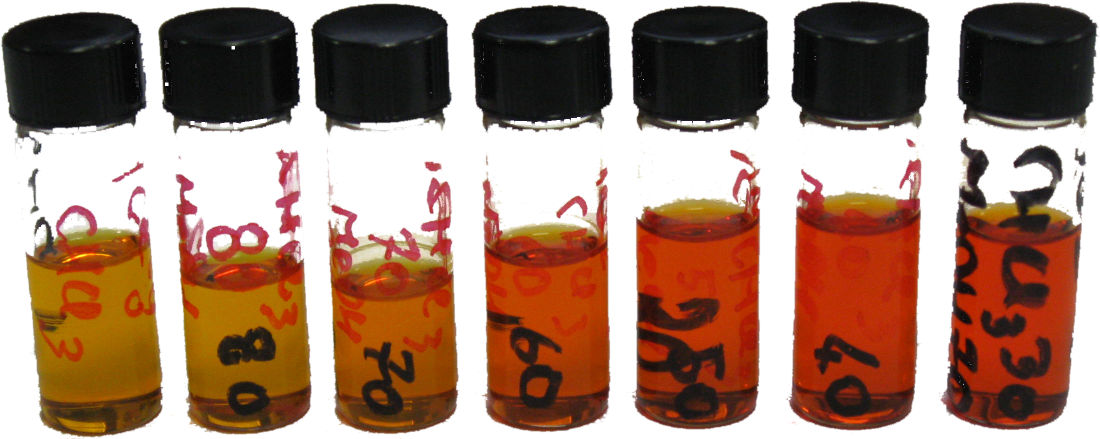
\includegraphics[width=0.7\textwidth]{ig2-8-vis-chcl3-meoh.jpg}
\caption[Photography of \cmpd+{ig2-8} in chloro\-form-methanol mixtures.]{Photography of \cmpd+{ig2-8} in chloro\-form-methanol mixtures. From left to right (and RGB color descriptions): in \ch{CHCl3} (red 59~\%, green 41~\%), \ch{MeOH} 20~\% (red 61~\%, green 39~\%), \ch{MeOH} 30~\% (red 67~\%, green 33~\%), \ch{MeOH} 40~\% (red 73~\%, green 27~\%), \ch{MeOH} 50~\% (red 78~\%, green 22~\%), \ch{MeOH} 60~\% (red 80~\%, green 20~\%) and \ch{MeOH} 70~\% (red 82~\%, green 18~\%).}
\label{fig:ig2-8-vis-chcl3-meoh}
\end{figure}

Adding some poor solvent to a solution of polymer leads to an aggregation, this can be simply identified by looking at the color of the solutions as shown in Figure~\ref{fig:ig2-8-vis-chcl3-meoh}. 
The obtained aggregates spontaneously precipitate within some hours or days forming a flocculate, this can affect the recording of the spectra.

We noticed that \cmpd+{ig2-4} (fixed concentration \SI{137}{\mg\per\liter}, \SI{\approx0.75}{\milli\Molar} in monomeric units) in chloroform shows a small absorbance shift when a poor solvent like methanol was added (\ch{MeOH} 0~\% \SI{430}{\nm}, \ch{MeOH} 50~\% \SI{433}{\nm}, \ch{MeOH} 60~\% \SI{435}{\nm} and \ch{MeOH} 70~\% \SI{434}{\nm}) while an extensive aggregation and precipitation occurred as revealed by the scattering baseline of sample in 70~\% of methanol (spectra are reported in appendix). 
The absence of a significant peak shift indicates the lack of exciton coupling or conjugation extension in aggregated form compared to solubilized form (maybe the conjugation length is limited by the very small molecular weight, see \gls{SEC} chromatogram in Figure~\ref{fig:ig2-4-ig2-8-sec-chcl3}). At high methanol concentrations a new peak at \SI{330}{\nm} rises, this peak is not assigned. 

As stated before, acetonitrile is a poor solvent for our polymers. Adding acetonitrile to a chloroform solution of polymer \cmpd+{ig2-15} until 1:1 ratio of good-poor solvent resulted in a red-shift of \SI{17}{\nm} (\SI{447}{\nm} $\rightarrow$ \SI{464}{\nm}) due to chain conjugation extension and exciton coupling in the aggregated state. 
Adding acetonitrile to a tetrahydrofuran solution caused a red-shift of \SI{17}{\nm} (\SI{449}{\nm} $\rightarrow$ \SI{466}{\nm}).
When methanol is used as a poor solvent together with tetrahydrofuran a \SI{17}{\nm} red-shift occur adding just 30~\% of non-solvent (\SI{449}{\nm} $\rightarrow$ \SI{466}{\nm}). 
Adding 10~\% more methanol resulted in further \SI{5}{\nm} shift (\SI{466}{\nm} $\rightarrow$ \SI{471}{\nm}). These data suggests that tetrahydrofuran is a worse solvent than chloroform and methanol is worse than acetonitrile.

We notice that when a non-solvent is added the peak at $\approx$~\SI{265}{\nm} becomes weaker, thus supporting the hypothesis that this peak is related to non-conjugated thio\-phene rings (expressed in page~\pageref{peak-265}).

\Gls{UVvis} measurement for \cmpd+{ig2-8} were performed at constant polymer concentration (\SI{137}{\mg\per\liter}, \SI{0.75}{\milli\Molar} in monomeric units, \SI{\approx1e-5}{\Molar} in polymeric chains) both in chloro\-form-methanol and chloro\-form-aceto\-nitrile using a \SI{1}{\mm} cuvette. 
In chloro\-form-methanol until 30~\% \ch{MeOH} no variation in the spectra was observed (\SI{445}{\nm} $\rightarrow$ \SI{444}{\nm}) then at 40~\% \ch{MeOH} a shift of \SI{14}{\nm} can be noticed (\SI{445}{\nm} $\rightarrow$ \SI{459}{\nm}) and the peak at short wavelengths (\SI{265}{\nm}) starts to weaken, see Figure~\ref{fig:ig2-8-uvvis-meoh}. 
Adding more methanol (while keeping constant polymer concentration) the peak energy varies slightly (\SI{459}{\nm} $\rightarrow$ \SI{462}{\nm}) but the absorptivity increases from \SI{8300}{\per\Molar\per\cm} up to \SI{13000}{\per\Molar\per\cm}. Repeating the measurement of the sample with 70~\% \ch{MeOH} after a day resulted in no variation of the absorption spectra (after re\-dispersion of the sample).

The fact that a clear iso\-sbestic point is missing in Figure~\ref{fig:ig2-8-uvvis-meoh} suggests that the transition isn't a simple one-step process. 

\begin{figure}[tbp]%ig2-8-uvvis-meoh
\begin{tikzpicture}
\begin{axis}[axis x line=bottom,axis y line=left,enlarge x limits=false,enlarge y limits=false,width=1\textwidth,height=8cm,xlabel=Wavelength (nm),ylabel=Molar absorptivity (\SI{}{\per\Molar\per\cm}),xmin=240,cycle list name=linestyles*,legend pos=north west,legend style={font=\footnotesize}]
\addplot table[y expr=\thisrowno{1}/0.0000753] {img/results/ig2-8-uvvis-137-chcl3-for-meoh.txt};
\addlegendentry{\cmpd+{ig2-8} in \ch{CHCl3}};
\addplot table[y expr=\thisrowno{1}/0.0000753] {img/results/ig2-8-uvvis-137-chcl3-70-meoh-30.txt};
\addlegendentry{\ch{CHCl3} 70 \% - \ch{MeOH} 30 \%};
\addplot table[y expr=\thisrowno{1}/0.0000753] {img/results/ig2-8-uvvis-137-chcl3-60-meoh-40.txt};
\addlegendentry{\ch{CHCl3} 60 \% - \ch{MeOH} 40 \%};
\addplot table[y expr=\thisrowno{1}/0.0000753] {img/results/ig2-8-uvvis-137-chcl3-50-meoh-50.txt};
\addlegendentry{\ch{CHCl3} 50 \% - \ch{MeOH} 50 \%};
\addplot table[y expr=\thisrowno{1}/0.0000753] {img/results/ig2-8-uvvis-137-chcl3-40-meoh-60.txt};
\addlegendentry{\ch{CHCl3} 40 \% - \ch{MeOH} 60 \%};
\addplot[densely dotted] table[y expr=\thisrowno{1}/0.0000753] {img/results/ig2-8-uvvis-137-chcl3-30-meoh-70.txt};
\addlegendentry{\ch{CHCl3} 30 \% - \ch{MeOH} 70 \%};
\end{axis}
\end{tikzpicture} \caption[UV-vis spectra of \cmpd+{ig2-8} in chloro\-form-methanol mixtures.]{\gls{UVvis} spectra of \cmpd+{ig2-8} in chloro\-form-methanol mixtures. Concentration \SI{137}{\mg\per\liter}. Pathlength \SI{1}{\mm}.}
\label{fig:ig2-8-uvvis-meoh}
\end{figure}

In chloro\-form-aceto\-nitrile \cmpd+{ig2-8} didn't show the absorption intensity enhancement shown in chloro\-form-methanol. Passing from chloroform solution to 40~\% acetonitrile a \SI{23}{\nm} red-shift was observed (\SI{444}{\nm} $\rightarrow$ \SI{467}{\nm}). 
Adding more acetonitrile the peak wavelength didn't change, no iso\-sbestic point can be seen. \label{uvvis-ch3cn} The longer wavelength obtained from aggregation in acetonitrile compared with aggregation in methanol (see Table~\ref{tab:bandgap} on page~\pageref{tab:bandgap}) could indicate a different aggregation geometry, this will be further investigated with circular dichroism spectroscopy in Section~\ref{sec:cd-poor}. 

The largest red-shift we observed with our polymers (\SI{23}{\nm}) is still smaller than some of the values reported in the literature for aggregated regioregular poly\-thio\-phenes.\superfootcite{McCullough1993}\superfootcite{Goto2002}\superfootcite{Kiriy2003}\superfootcite{Shi2006} This could point to a different organization with a lesser degree of planarization or $\pi-\pi$ stacking.

\end{subsubsection}
\begin{subsubsection}{In Solid State}

\begin{table}%bandgap
\centering
\caption[UV-vis data and estimated band gaps for samples of \cmpd+{ig2-4}, \cmpd+{ig2-15} and \cmpd+{ig2-8}.]{\gls{UVvis} data and estimated band gaps for polymers \cmpd+{ig2-4}, \cmpd+{ig2-15} and \cmpd+{ig2-8}.}\label{tab:bandgap}
\begin{tabular}{c|c|c|c|c}
\toprule
polymer&processing&\tallcell{\gls{UVvis} peak\\(\SI{}{\nm})}&\tallcell{\gls{UVvis} onset\\ (\SI{}{\nm})}&\tallcell{Band gap\\(\SI{}{\eV})} \\ \cmidrule{1-5}
\multirow{3}{*}{\cmpd+{ig2-4}}&\ch{CHCl3} solution	&430	&523	&2.37	 		 	\\ 
&spin \SI{700}{\rpm} from \ch{CHCl3}	&$\approx462$	&574	&2.16	 	\\
&in \ch{KCl}&$\approx464$	&&	\\ \cmidrule{1-1}
\multirow{4}{*}{\cmpd+{ig2-15}}&\ch{CHCl3} solution	&446	&531	&2.33	 		 	\\ 
&\gls{THF} solution		&450&533	&2.33	 \\
&cast from \ch{CH2Cl2}&$\approx486$	&589	&2.10		\\ 
&in \ch{KCl}&$\approx493$	&&	\\\cmidrule{1-1}
\multirow{8}{*}{\cmpd+{ig2-8}}&\ch{CHCl3} solution	&444	&528	&2.35	 		 	\\
&cast from \ch{CHCl3}	&$\approx471$	&584&2.12\\
&cast from \gls{THF}		&$\approx473$	&581&2.13 \\
&cast from \ch{CH2Cl2}	&$\approx469$	&577&2.15	\\
&spin \SI{700}{\rpm} from \ch{CHCl3}	&$\approx476$	&571&2.17	\\
&spin \SI{700}{\rpm} from \gls{THF}	&$\approx476$	&566&2.19	\\
&spin \SI{1000}{\rpm} from \ch{CHCl3}&$\approx492$	&587&2.11	\\
&in \ch{KCl}&$\approx495$	&&	\\

\bottomrule
\end{tabular}
\end{table}

\label{ig2-4-uvvis}
\cmpd+{ig2-4} was analyzed in a thin film spin coated (\SI{700}{\rpm}) from chloroform solution. While only a small red-shift was observed passing from chloroform solution to chloro\-form-methanol mixtures (\SI{430}{\nm} $\rightarrow$ \SI{434}{\nm}), in the \gls{UVvis} spectrum of this thin film (reported in appendix), a \SI{32}{\nm} red-shift was observed (\SI{430}{\nm} $\rightarrow$ \SI{462}{\nm}). This fact suggests that the aggregation obtained in 70~\% \ch{MeOH} doesn't imply a good packing of chains while this takes place in solid state.

\begin{figure}[tbp]%ig2-15-uvvis-film
\begin{tikzpicture}
\begin{axis}[axis x line=bottom,axis y line=left,enlarge x limits=false,enlarge y limits=false,yticklabels={,,},width=1\textwidth,height=6cm,xlabel=Wavelength (nm),ylabel=Absorbance,xmin=240,xmax=650,legend pos=north west,legend style={font=\footnotesize},cycle list name=linestyles*]
\addplot table[y expr=\thisrowno{1}/1.04169] {img/results/ig2-15-uvvis-chcl3.txt};
\addlegendentry{\cmpd+{ig2-15} in \ch{CHCl3}};
\addplot table[y expr=\thisrowno{1}/1.8789] {img/results/ig2-15-uvvis-thf-55-ch3cn-45.txt};
\addlegendentry{\gls{THF} 55 \% - \ch{CH3CN} 45 \%};
\addplot table[y expr=(\thisrowno{1}-0.15)/0.219712] {img/results/ig2-15-uvvis-cast-ch2cl2.txt};
\addlegendentry{cast from \ch{CH2Cl2}};
\end{axis}
\end{tikzpicture} \caption[UV-vis spectra of polymer \cmpd+{ig2-15} in solution and thin film.]{Normalized UV-vis spectra of polymer \cmpd+{ig2-15} in chloroform, in tetra\-hydro\-furan-aceto\-nitrile solution and thin film cast from a dichloromethane solution.}
\label{fig:ig2-15-uvvis-film}
\end{figure}

\label{ig2-15-uvvis-film}
In Figure~\ref{fig:ig2-15-uvvis-film} a strong red-shift is observed for \cmpd+{ig2-15} cast from dichloromethane (chloroform solution peak \SI{447}{\nm}, \gls{THF} 55~\% - \ch{MeOH} 45~\% \SI{466}{\nm}, cast from dichloromethane \SI{\approx486}{\nm}).

\label{ig2-8-film}
For \cmpd+{ig2-8} many films were analyzed, both from spin coating and from casting. 
The obtained films vary in thickness and the wavelength of the maximum absorption peak in their spectra also vary. 
Thin films from casting have a maximum absorption wavelength around \SI{\approx471}{\nm} (cast from \ch{CHCl3} \SI{\approx471}{\nm}, cast from \gls{THF} \SI{\approx473}{\nm}, cast from \ch{CH2Cl2} \SI{\approx469}{\nm}) while spin coated thin films are generally slightly red-shifted to \SI{\approx476}{\nm} (spin \SI{700}{\rpm} from \ch{CHCl3} \SI{\approx476}{\nm}, spin \SI{700}{\rpm} from \gls{THF} \SI{\approx476}{\nm}) with only a case of film resulting in a very strong red-shift to \SI{\approx492}{\nm} (spin \SI{1000}{\rpm} from \ch{CHCl3}). These \gls{UVvis} spectra are reported in appendix. 
These values are somewhat different from peak wavelengths of colloidal dispersions in solvent-non-solvent mixtures (\ch{CHCl3} - \ch{MeOH} \SI{\approx462}{\nm}, \ch{CHCl3} - \ch{CH3CN} \SI{\approx468}{\nm}, \gls{THF} - \ch{CH3CN} \SI{467}{\nm}, see Table~\ref{tab:bandgap}). The out\-lier film (spin \SI{1000}{\rpm} from \ch{CHCl3}) also showed a weaker absorption at short wavelengths (\SI{265}{\nm}). The fact that all spin coated films are red-shifted relatively to all cast films 
means that a fast spin coating forces the chains to stretch and flatten on the quartz substrate while a slow deposition allows the chains to aggregate in a preferred organization with shorter conjugation length or a worse packing. 

Thin films from similar polythio\-phenes bearing unbranched side chains\superfootcite{Zoombelt2008} showed a lower $\pi-\pi^*$ transition energy (\SI{500}{\nm}). This could be related to a worse exciton coupling in our chiral polythio\-phenes or to a worse packing caused by the branching of our side chains.

\label{uvvis-pentane}
Dipping our films in a side groups-selective solvent could give a reorganization of side chains helping the reaching of a more ordered arrangement of the macromolecules.\superfootcite{Caronna1997}\superfootcite{Salatelli2010} Indeed no change in main peak absorption was observed when spin coated films were dipped in pentane; only the \SI{265}{\nm} weak peak, where present, decreased in intensity (that could be related to ordering of non-conjugated rings, see page~\pageref{peak-265}). 

The fact that we could not observe a vibronic fine structure in any of the spectra of our samples, suggests a lack of crystallinity,\superfootcite{Brown2003}\superfootcite{Zoombelt2008} as will be further 
investigated in Section~\ref{xrd}.

The band gap in solution can be estimated from onset of \gls{HOMO}-\gls{LUMO} transition (a $\pi \rightarrow \pi^*$ transition) in \gls{UVvis} spectra. The utilized onset point was the point where line tangent to the peak's right inflection point intersect the baseline. The results are reported in Table~\ref{tab:bandgap}. 

Polymers were analyzed also in \ch{KCl} disks (dried from chloroform with a nitrogen flux, ground with \ch{KCl} and pressed). The obtained disks weren't homogeneous thus a strong scattering was the issue with these measurements. %was noticed in Figure~\ref{fig:uvvis-kcl}.
In disks from \cmpd+{ig2-4} no wavelength change was observed comparing to the spin coated thin film. 
Both \cmpd+{ig2-15} and \cmpd+{ig2-8} have a main peak wavelength around \SI{495}{\nm} and we can notice (see Table~\ref{tab:bandgap}) a red-shift referring to \SI{700}{\rpm} spin coated and cast films. The facts that \cmpd+{ig2-8} peak position in \ch{KCl} isn't significantly different from \SI{1000}{\rpm} spin coated film and that peak of \cmpd+{ig2-4} in \ch{KCl} isn't different from \cmpd+{ig2-4} spin coated prompt us to believe that drying the samples with a nitrogen flux had the same effect of a fast spin coating on polymers. But we can't exclude that an aggregation change could be due to sintering of the polymer due to the huge pressure used to produce \ch{KCl} disks.\superfootcite{Loi2001} 

\end{subsubsection}
\end{subsection}
\clearpage
\begin{subsection}{Photoluminescence Spectroscopy Characterization}
\label{sec:pl}

\begin{subsubsection}{In a Good Solvent}

\begin{figure}[tbp]%pl-vs-uvvis
\begin{tikzpicture}
\begin{axis}[axis x line=bottom,axis y line=left,enlarge x limits=false,enlarge y limits=false,width=1\textwidth,height=8cm,xlabel=Wavelength (nm),ylabel=Absorption (a.\ u.),xmin=300,xmax=800,yticklabels={,,},legend entries={\cmpd{ig2-4} in \ch{CHCl3},\cmpd{ig2-15} in \ch{CHCl3},\cmpd{ig2-8} in \ch{CHCl3}}]
\addplot[solid] table[y expr=\thisrowno{1}*100] {img/results/ig2-4-uvvis-chcl3.txt};
\addplot[dashed] table[y expr=\thisrowno{1}*127] {img/results/ig2-15-uvvis-chcl3.txt};
\addplot[dotted] table[y expr=\thisrowno{1}*215] {img/results/ig2-8-uvvis-137-chcl3-for-meoh.txt};
\node at (axis cs:600,15) {emission};
\node at (axis cs:430,15) {absorption};
\end{axis}
\begin{axis}[axis x line=none,axis y line=right,enlarge x limits=false,enlarge y limits=false,width=1\textwidth,height=8cm,ylabel=Photoluminescence (a.\ u.),xmin=300,xmax=800]
\addplot[solid] table {img/results/ig2-4-pl-5480-chcl3.txt};
\addplot[dashed] table {img/results/ig2-15-pl-5480-chcl3.txt};
\addplot[dotted] table {img/results/ig2-8-pl-5480-chcl3.txt};
\end{axis}
\end{tikzpicture} \caption[Photoluminescence and absorption of \cmpd+{ig2-4}, \cmpd+{ig2-15} and \cmpd+{ig2-8} chloroform solutions.]{Photoluminescence and absorption of \cmpd+{ig2-4}, \cmpd+{ig2-15} and \cmpd+{ig2-8} chloroform solutions. Concentration for photoluminescence samples is \SI{5.48}{\g\per\liter}. Absorption spectra are rescaled to \gls{PL} intensity.}
\label{fig:pl-vs-uvvis}
\end{figure}

In a good solvent like chloroform, \cmpd+{ig2-15} and \cmpd+{ig2-8} have similar photoluminescence spectra (see Figure~\ref{fig:pl-vs-uvvis}) when stimulated at \SI{450}{\nm}. This was expected because in solution the chirality of side chains shouldn't influence to a big extent the conjugated backbone which is responsible for absorption and emission. 
\cmpd+{ig2-4} in chloroform shows a lower fluorescence efficiency (see Figure~\ref{fig:pl-vs-uvvis}).
For each polymer increasing by 40 times the concentration had no effect on fluorescence spectra except for a small decrease of emission maybe due to interaction between chains, not yet an aggregation, or due to auto-absorption (as shown in Figure~\ref{fig:pl-vs-uvvis}, the superposition of absorption and emission spectra is tiny, thus an auto-absorption by F\"{o}rster resonance energy transfer should have a limited importance). 
All the polymers show fluorescence maximum at about the same wavelength (\SI{575}{\nm}) with an intense shoulder at lower energies (\SI{600}{\nm}). Usually in poly\-thio\-phenes this shoulder is assigned to a small extent of aggregation present even in good solvent or to a vibronic band. No similar vibronic shoulder was seen in absorption spectra. Another possibility is that the two peaks could originate from different molecular structures, for example from two different molecular weights (see Section~\ref{sec:weight} for results on weight), with the emission from the low weight fraction pumping energy in the absorbance of the high weight fraction via a F\"{o}rster resonance energy transfer. Moreover we can hypothesize the presence of different chain conformations in solution. 

The Stokes shift\nota{\textit{Stokes shift} is the difference (in wavelength or frequency units) between positions of the band maxima of the absorption and emission spectra (fluorescence and Raman being two examples) of the same electronic transition. (Wikipedia)} 
is about \SI{0.63}{\eV} (absorption \SI{\approx445}{\nm}, \SI{2.79}{\eV}, emission \SI{\approx575}{\nm}, \SI{2.16}{\eV}), comparable with other poly\-thio\-phenes.\superfootcite{Langeveld-Voss1996}\superfootcite{Xu1993}\superfootcite{Theander1999}\superfootcite{Ohshimizu2008}\superfootcite{Higashihara2011}\superfootcite{Bouman1994a}

\end{subsubsection}
\begin{subsubsection}{In Mixtures of Good and Poor Solvents}

\begin{figure}[tbp]%ig2-8-pl365-chcl3-meoh
\centering
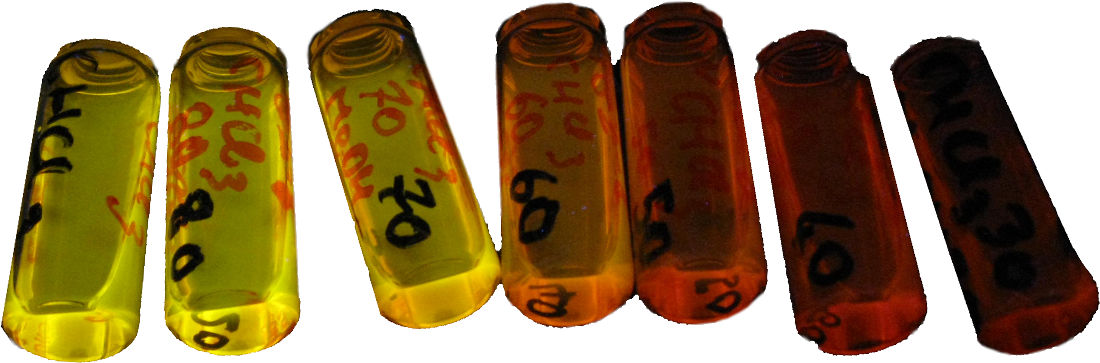
\includegraphics[width=0.7\textwidth]{ig2-8-pl365-chcl3-meoh.jpg}
\caption[Photography of photoluminescence of \cmpd+{ig2-8} in chloro\-form-methanol mixtures.]{Photography of photoluminescence of \cmpd+{ig2-8} in chloro\-form-methanol mixtures illuminated at \SI{365}{\nm}. From the left to the right: in \ch{CHCl3}, \ch{MeOH} 20~\%, \ch{MeOH} 30~\%, \ch{MeOH} 40~\%, \ch{MeOH} 50~\%, \ch{MeOH} 60~\% and \ch{MeOH} 70~\%.}
\label{fig:ig2-8-pl365-chcl3-meoh}
\end{figure}

\begin{figure}[tbp]%ig2-15-pl
\begin{tikzpicture}
\begin{axis}[axis x line=bottom,axis y line=left,enlarge x limits=false,enlarge y limits=false,width=1\textwidth,height=6cm,xlabel=Wavelength (nm),ylabel=Photoluminescence (a.\ u.),xmin=480,cycle list name=linestyles*]
\addplot table {img/results/ig2-15-pl-137-chcl3.txt};
\addlegendentry{\cmpd+{ig2-15} in \ch{CHCl3}};
\addplot table {img/results/ig2-15-pl-137-chcl3-75-meoh-25.txt};
\addlegendentry{in \ch{CHCl3} 75 \% - \ch{MeOH} 25 \%};
\addplot table {img/results/ig2-15-pl-137-chcl3-50-meoh-50.txt};
\addlegendentry{in \ch{CHCl3} 50 \% - \ch{MeOH} 50 \%};
\addplot table {img/results/ig2-15-pl-137-chcl3-30-meoh-70.txt};
\addlegendentry{in \ch{CHCl3} 30 \% - \ch{MeOH} 70 \%};
\end{axis}
\end{tikzpicture} \caption[Photoluminescence of \cmpd+{ig2-4} in chloro\-form-methanol mixtures.]{Photoluminescence of \cmpd+{ig2-4} in chloro\-form-methanol mixtures. Concentration \SI{137}{\mg\per\liter}.}
\label{fig:ig2-15-pl}
\end{figure}

\begin{figure}[tbp]%ig2-8-pl
\begin{tikzpicture}
\begin{axis}[axis x line=bottom,axis y line=left,enlarge x limits=false,enlarge y limits=false,width=1\textwidth,height=6cm,xlabel=Wavelength (nm),ylabel=Photoluminescence (a.\ u.),xmin=480,cycle list name=linestyles*]
\addplot table {img/results/ig2-8-pl-137-chcl3.txt};
\addlegendentry{\cmpd+{ig2-8} in \ch{CHCl3}};
\addplot table {img/results/ig2-8-pl-137-chcl3-75-meoh-25.txt};
\addlegendentry{in \ch{CHCl3} 75 \% - \ch{MeOH} 25 \%};
\addplot table {img/results/ig2-8-pl-137-chcl3-50-meoh-50.txt};
\addlegendentry{in \ch{CHCl3} 50 \% - \ch{MeOH} 50 \%};
\addplot table {img/results/ig2-8-pl-137-chcl3-30-meoh-70.txt};
\addlegendentry{in \ch{CHCl3} 30 \% - \ch{MeOH} 70 \%};
\end{axis}
\end{tikzpicture} \caption[Photoluminescence of \cmpd+{ig2-8} in chloro\-form-methanol mixtures]{Photoluminescence of \cmpd+{ig2-8} in chloro\-form-methanol mixtures. Concentration \SI{137}{\mg\per\liter}.}
\label{fig:ig2-8-pl}
\end{figure}

\begin{figure}[tbp]%ig2-8-ig2-15-pl
\begin{tikzpicture}
\begin{axis}[axis x line=bottom,axis y line=left,enlarge x limits=false,enlarge y limits=false,width=1\textwidth,height=6cm,xlabel=Wavelength (nm),ylabel=Photoluminescence (a.\ u.),xmin=480,legend style={font=\footnotesize},cycle list name=linestyles*]
\addplot table {img/results/ig2-15-pl-137-chcl3-30-meoh-70.txt};
\addlegendentry{\cmpd+{ig2-15} in \ch{CHCl3} 30 \% - \ch{MeOH} 70 \%};
\addplot table {img/results/ig2-8-pl-137-chcl3-50-meoh-50.txt};
\addlegendentry{\cmpd+{ig2-8} in \ch{CHCl3} 50 \% - \ch{MeOH} 50 \%};
\addplot table {img/results/ig2-8-pl-137-chcl3-30-meoh-70.txt};
\addlegendentry{\cmpd+{ig2-8} in \ch{CHCl3} 30 \% - \ch{MeOH} 70 \%};
\end{axis}
\end{tikzpicture} \caption[Photoluminescence of \cmpd+{ig2-15} and \cmpd+{ig2-8} in chloro\-form-methanol mixtures.]{Comparison of photoluminescence of \cmpd+{ig2-15} and \cmpd+{ig2-8} in chloro\-form-methanol mixtures. Spectra are not rescaled, concentration is \SI{137}{\mg\per\liter} for both \cmpd+{ig2-15} and \cmpd+{ig2-8}.}
\label{fig:ig2-8-ig2-15-pl}
\end{figure}

As it's clear by looking at Figure~\ref{fig:ig2-8-pl365-chcl3-meoh}, the addition of methanol to polymer solutions in chloroform produces a quenching in the fluorescence due to the formation of aggregated states with very low quantum efficiency.

Adding 50~\% of methanol to a chloroform solution of polymer \cmpd+{ig2-4} induces only a small change in photoluminescence spectra, just a reduction of the shoulder at longer wavelength.

Adding 25~\%, 50~\%, 70~\% of methanol to a chloroform solution of \cmpd+{ig2-15} resulted in a progressive quenching of photoluminescence, both for the main emission peak and of the shoulder (see Figure~\ref{fig:ig2-15-pl}). 
Measuring again these samples after an hour resulted in a diminished fluorescence (approximately of 10 - 25~\%) maybe due the greater degree of ordering reached by the aggregates. The absence of a strong quenching of photoluminescence indicates the presence of non well-packed chains.

In every spectra the position of the peaks is unvaried compared with photoluminescence of polymer in chloroform, but the relative intensity of the main peak and the shoulder varies. Adding methanol both peak show a decreased intensity but the quenching of the higher energy peak is more important than for the shoulder. In 70~\% of methanol the two peaks from \cmpd+{ig2-15} have the same fluorescence intensity. 

\cmpd+{ig2-8} in a mixture of chloroform with 25~\% methanol gives a fluorescence spectra identical to \cmpd+{ig2-15} in 25~\% methanol. The further addition of methanol to solutions of \cmpd+{ig2-8} (see Figure~\ref{fig:ig2-8-pl}) has a rather different effect: a dramatic quenching of fluorescence and a strong red-shift of the emission. 
This behavior can be noted also from Figure~\ref{fig:ig2-8-pl365-chcl3-meoh} where \cmpd+{ig2-8} is illuminated with a common \SI{365}{\nm} lamp. In Figure~\ref{fig:ig2-8-ig2-15-pl} is reported a comparison between \gls{PL} of \cmpd+{ig2-15} and \cmpd+{ig2-8} at high methanol percents. The new peak at long wavelengths could be assigned to aggregated species, it was not distinguishable in the previous spectra because of the more intense emission of non aggregated chains. 
The non enantio\-purity of \cmpd+{ig2-15} can be regarded as a degree of disorder that can interfere with the ordering needed for the formation of aggregates.

\end{subsubsection}
\begin{subsubsection}{In Solid State}

Up to now no measurement of photoluminescence on thin film was performed because of their very weak stimulated emission.

\end{subsubsection}
\end{subsection}
\clearpage
\begin{subsection}{Circular Dichroism Spectroscopy Characterization}
\begin{subsubsection}{In a Good Solvent}

Both \cmpd+{ig2-15} in tetrahydrofuran and \cmpd+{ig2-8} in chloroform showed a non zero circular dichroism signal. The signal is extremely weak but we can recognize a bisignate peak 
with the inflection point located around the \gls{UVvis} main absorption peak. These signals may recall a 
positive bisignate circular dichroism couplet (the sign of a bisignate couplet is defined as the sign of the long wavelength part of this couplet; the bisignate peak inflection point and amplitude were obtained fitting the peak with a sine waveform, see page~\pageref{fitting}). 

\end{subsubsection}
\begin{subsubsection}{In Mixtures of Good and Poor Solvents}
\label{sec:cd-poor}

\begin{table}%soluzioni-cd
\centering
\caption[UV-vis and CD data of \cmpd+{ig2-15} and \cmpd+{ig2-8} solutions.]{\gls{UVvis} and \gls{CD} data of \cmpd+{ig2-15} and \cmpd+{ig2-8} solutions.}\label{tab:soluzioni-cd}
\begin{tabular}{c|c|c|c|c}
\toprule
processing&\tallcell{UV-vis\\ peak\\(\SI{}{nm})}&\tallcell{CD\\ inflection\\(\SI{}{nm})}&\tallcell{CD\\ amplitude\\(\SI{}{mdeg})}&\tallcell{molar\\ circular\\ dichroism\\ ($\Delta\epsilon$, \\ \SI{}{\per\Molar\per\cm})}\\ \cmidrule{1-5}
\cmpd+{ig2-15}					&\multicolumn{4}{c}{}\\ \cmidrule{1-1}
\ch{CHCl3} solution						&446&	&0	&0\\
\gls{THF} solution							&450&	&	 &	\\
\ch{CHCl3} 70\% \ch{MeOH} 30\%	&446&$\approx460$&0.5&0.2	\\
\ch{CHCl3} 70\% \ch{MeOH} 30\% \SI{30}{\minute}&$\approx446$&457&1	 &0.4	\\
\ch{CHCl3} 50\% \ch{MeOH} 50\%	&$\approx466$	&459&7.7	 &3.1	\\
\ch{CHCl3} 40\% \ch{CH3CN} 60\%&$\approx469$&454&2.3	 &0.9	\\ 
\ch{CHCl3} 30\% \ch{CH3CN} 70\%&$\approx469$&460&4.8	 &1.9	\\
\ch{CHCl3} 20\% \ch{CH3CN} 80\%&$\approx469$&460&4.8	 &1.9	\\
\ch{CHCl3} 10\% \ch{CH3CN} 90\%&$\approx470$	&460&4.1	 &1.7	\\
\gls{THF} 60\% \ch{CH3CN} 40\%	&$\approx466$&458&5.2	 &2.1	\\
\gls{THF} 50\% \ch{CH3CN} 50\%	&469&458&4	 &1.6	\\
\gls{THF} 50\% \ch{CH3CN} 50\% \SI{274}{\mg/\liter}&466&458&11.4	 &2.3	\\
\gls{THF} 50\% \ch{CH3CN} 50\% \SI{548}{\mg/\liter}&469&459&26.2	 &2.6	\\
\gls{THF} 40\% \ch{CH3CN} 60\%	&$\approx468$&456&2.8	&1.1	\\
\gls{THF} 20\% \ch{CH3CN} 80\%	&$\approx470$&459&3	 &1.2\\ \cmidrule{1-5}
\cmpd+{ig2-8}					&\multicolumn{4}{c}{}\\ \cmidrule{1-1}
\ch{CHCl3} solution 						&444	&	&0	&0	\\
\ch{CHCl3} 70\% \ch{MeOH} 30\%	&$\approx443$&&0&0\\
\ch{CHCl3} 70\% \ch{MeOH} 30\% \SI{10}{\minute}&$\approx447$&441&6.1&2.5\\
\ch{CHCl3} 70\% \ch{MeOH} 30\% \SI{30}{\minute}&443&445&3.5&1.4\\
\ch{CHCl3} 70\% \ch{MeOH} 30\% \SI{1}{\day}&$\approx443$&443&22.9&9.4\\
\ch{CHCl3} 60\% \ch{MeOH} 40\%	&459&456&13.8&5.5\\
\ch{CHCl3} 50\% \ch{MeOH} 50\%	&461&457&15.6&6.4\\
\ch{CHCl3} 40\% \ch{MeOH} 60\%	&462&456&19.6&7.9\\
\ch{CHCl3} 30\% \ch{MeOH} 70\%	&462&456&24&9.7\\
\ch{CHCl3} 40\% \ch{CH3CN} 60\%	&467&458&7.3&2.9\\
\ch{CHCl3} 30\% \ch{CH3CN} 70\%	&465&458&12.4&5.0\\
\ch{CHCl3} 20\% \ch{CH3CN} 80\%	&467&459&10.1&4.1\\
\ch{CHCl3} 10\% \ch{CH3CN} 90\%	&469&459&6.5&2.6\\
\gls{THF} 60\% \ch{CH3CN} 40\%	&$\approx466$&457&6.4&2.6\\
\gls{THF} 50\% \ch{CH3CN} 50\%	&$\approx468$&457&5.5&2.2\\
\gls{THF} 40\% \ch{CH3CN} 60\%	&$\approx467$&457&7.0&2.8\\
\gls{THF} 20\% \ch{CH3CN} 80 \%	&$\approx467$&458&8.2&3.3\\
\bottomrule
\end{tabular}

\smallskip

{Where not specified a \SI{137}{\mg\per\liter} concentration was used.}
\end{table}

In chloro\-form-methanol mixtures, \cmpd+{ig2-4} showed at first (100~\% chloroform) a dichroic monosignate negative peak in the region of the main \gls{UVvis} absorption, then increasing methanol content, a bisignate peak appeared.

This positive bisignate circular dichroism couplet, that is what we detect for all our polymers in the aggregated form, could rise from intramolecular or intermolecular interactions. Referring to the latter case a positive couplet is reported as being produced by two close identical chromophores with a right handed relative orientation,\superfootcite{Berova2007} this is confirmed by experiments on oligo\-thio\-phene with a known relative orientation.\superfootcite{Langeveld-Voss1998} 

\begin{figure}[tbp]%ig2-15-cd-meoh
\begin{tikzpicture}
\begin{axis}[axis x line=bottom,axis y line=left,enlarge x limits=false,enlarge y limits=true,width=1\textwidth,height=6cm,xlabel=Wavelength (nm),ylabel=Molar circular dichroism $\Delta\epsilon$,xmin=240,legend pos=north west,cycle list name=linestyles*]
\addplot table[y expr=\thisrowno{1}*0.403] {img/results/ig2-15-cd-137-chcl3-70-meoh-30.txt};
\addlegendentry{in \ch{CHCl3} 70 \% - \ch{MeOH} 30 \%};
\addplot table[y expr=\thisrowno{1}*0.403] {img/results/ig2-15-cd-137-chcl3-70-meoh-30-30min.txt};
\addlegendentry{in \ch{CHCl3} 70 \% - \ch{MeOH} 30 \% \SI{30}{\minute}};
\addplot table[y expr=\thisrowno{1}*0.403] {img/results/ig2-15-cd-137-chcl3-50-meoh-50.txt};
\addlegendentry{in \ch{CHCl3} 50 \% - \ch{MeOH} 50 \%};
\end{axis}
\end{tikzpicture} \caption[Circular dichroism of \cmpd+{ig2-15} in chloro\-form-methanol mixtures.]{Circular dichroism of \cmpd+{ig2-15} in chloro\-form-methanol mixtures. Concentration \SI{137}{\mg\per\liter}, pathlength \SI{1}{\mm}. Molar circular dichroism is referred to the quantity of thio\-phene rings; $\Delta\epsilon = \theta (\mathrm{mdeg}) / (32982 \cdot l (\mathrm{cm}) \cdot c (\mathrm{mol/L}))$.}
\label{fig:ig2-15-cd-meoh}
\end{figure}

In contrast with measurement on \cmpd+{ig2-4}, \cmpd+{ig2-15} doesn't show any monosignate circular dichroism (CD) peak. As shown in Figure~\ref{fig:ig2-15-cd-meoh}, adding 30~\% of methanol to a chloroform solution generates only an extremely weak bisignate signal at first (amplitude \SI{0.5}{mdeg}), but it was sufficient to wait half an hour to see a clear dichroic signal rising. Adding more methanol resulted in strong enhancement of circular dichroism. 
Looking at the bisignate couplet inflection points and \gls{UVvis} peak wavelengths 
we notice no variation in inflection points (\SI{457}{\nm} for \ch{MeOH} 30~\% \SI{30}{\minute}, \SI{459}{\nm} for \ch{MeOH} 50~\%) while a \SI{20}{\nm} red shift is observed in \gls{UVvis} spectra. 
All the significant numeric data for \gls{UVvis} and \gls{CD} characterization in solution are reported in Table~\ref{tab:soluzioni-cd}.

\begin{figure}[tbp]%ig2-15-cd-ch3cn
\begin{tikzpicture}
\begin{axis}[axis x line=bottom,axis y line=left,enlarge x limits=false,enlarge y limits=true,width=1\textwidth,height=8cm,xlabel=Wavelength (nm),ylabel=Molar circular dichroism $\Delta\epsilon$,xmin=240,legend pos=north west,cycle list name=linestyles*]
\addplot table[y expr=\thisrowno{1}*0.403] {img/results/ig2-15-cd-137-chcl3-40-ch3cn-60.txt};
\addlegendentry{in \ch{CHCl3} 40 \% - \ch{CH3CN} 60 \%};
\addplot table[y expr=\thisrowno{1}*0.403] {img/results/ig2-15-cd-137-chcl3-30-ch3cn-70.txt};
\addlegendentry{in \ch{CHCl3} 30 \% - \ch{CH3CN} 70 \%};
\addplot table[y expr=\thisrowno{1}*0.403] {img/results/ig2-15-cd-137-chcl3-20-ch3cn-80.txt};
\addlegendentry{in \ch{CHCl3} 20 \% - \ch{CH3CN} 80 \%};
\addplot table[y expr=\thisrowno{1}*0.403] {img/results/ig2-15-cd-137-chcl3-10-ch3cn-90.txt};
\addlegendentry{in \ch{CHCl3} 10 \% - \ch{CH3CN} 90 \%};
\end{axis}
\end{tikzpicture} \caption[Circular dichroism of \cmpd+{ig2-15} in chloro\-form-aceto\-nitrile mixtures.]{Circular dichroism of \cmpd+{ig2-15} in chloro\-form-aceto\-nitrile mixtures. Concentration \SI{137}{\mg\per\liter}, pathlength \SI{1}{\mm}.}
\label{fig:ig2-15-cd-ch3cn}
\end{figure}

In chloro\-form-aceto\-nitrile mixtures passing from 60~\% to 70~\% of non solvent a clear shift of the bisignate couplet from \cmpd+{ig2-15} was noticed (\SI{454}{\nm} $\rightarrow$ \SI{460}{\nm}) joined with an increase of \gls{CD} intensity. Adding more non solvent the signal remains quite the same (see Figure~\ref{fig:ig2-15-cd-ch3cn}). During this addition the \gls{UVvis} spectra remains almost unchanged (see Table~\ref{tab:soluzioni-cd}). Interesting is the presence of a monosignate peak in correspondence with the \gls{UVvis} signal at \SI{270}{\nm}, likely related to non conjugated rings absorption (see page~\pageref{peak-265}).

\begin{figure}[tbp]%ig2-15-cd-thf-ch3cn
\begin{tikzpicture}
\begin{axis}[axis x line=bottom,axis y line=left,enlarge x limits=false,enlarge y limits=true,width=1\textwidth,height=8cm,xlabel=Wavelength (nm),ylabel=Molar circular dichroism $\Delta\epsilon$,xmin=240,legend style={font=\footnotesize},legend pos=north west,cycle list name=linestyles*]
\addplot table[y expr=\thisrowno{1}*0.403] {img/results/ig2-15-cd-137-thf-60-ch3cn-40.txt};
\addlegendentry{in \gls{THF} 60 \% - \ch{CH3CN} 40 \%};
\addplot table[y expr=\thisrowno{1}*0.403] {img/results/ig2-15-cd-137-thf-50-ch3cn-50.txt};
\addlegendentry{in \gls{THF} 50 \% - \ch{CH3CN} 50 \%};
\addplot table[y expr=\thisrowno{1}*0.201] {img/results/ig2-15-cd-274-thf-50-ch3cn-50.txt};
\addlegendentry{in \gls{THF} 50 \% - \ch{CH3CN} 50 \% \SI{274}{\mg\per\liter}};
\addplot table[y expr=\thisrowno{1}*0.101] {img/results/ig2-15-cd-548-thf-50-ch3cn-50.txt};
\addlegendentry{in \gls{THF} 50 \% - \ch{CH3CN} 50 \% \SI{548}{\mg\per\liter}};
\addplot table[y expr=\thisrowno{1}*0.403] {img/results/ig2-15-cd-137-thf-40-ch3cn-60.txt};
\addlegendentry{in \gls{THF} 40 \% - \ch{CH3CN} 60 \%};
\addplot[densely dotted] table[y expr=\thisrowno{1}*0.403] {img/results/ig2-15-cd-137-thf-20-ch3cn-80.txt};
\addlegendentry{in \gls{THF} 20 \% - \ch{CH3CN} 80 \%};
\end{axis}
\end{tikzpicture} \caption[Circular dichroism of \cmpd+{ig2-15} in tetra\-hydro\-furan-aceto\-nitrile mixtures.]{Circular dichroism of \cmpd+{ig2-15} in tetra\-hydro\-furan-aceto\-nitrile mixtures. Where not specified a concentration of \SI{137}{\mg\per\liter} was used. Pathlength \SI{1}{\mm}.}
\label{fig:ig2-15-cd-thf-ch3cn}
\end{figure}

\label{nonlinearita}
In order to discern if the interactions responsible of the \gls{CD} signal are intra-molecular or inter-molecular, the concentration dependence of the \gls{CD} spectrum of \cmpd+{ig2-15} in tetra\-hydro\-furan-aceto\-nitrile 50~\% - 50~\% was investigated (see Figure~\ref{fig:ig2-15-cd-thf-ch3cn} and data in Table~\ref{tab:soluzioni-cd}). 
A non linear dependence on concentration was found both for circular dichroism and for absorption intensities (confirmed by $g$ calculations, graph reported in appendix). The non linearity of \gls{UVvis} absorption is unexplained but the cooperative effect of the concentration on bisignate couplet amplitude suggests that the transition occurs inter-molecularly. 
Increasing the acetonitrile percent in tetra\-hydro\-furan-aceto\-nitrile mixtures results in a strong decrease of the \gls{CD} signal (see Figure~\ref{fig:ig2-15-cd-thf-ch3cn}) accompanied by a very small decrease in the \gls{UVvis} absorption peak, this is not unexpected and could be related to an extensive aggregation or to a change of the aggregate structure with coincident loss of the helical structure.\superfootcite{Zahn2002}

Adding 20~\% of methanol to a chloroform solution of \cmpd+{ig2-8} didn't generate any \gls{CD} signal, even after one day. Adding 30~\% of methanol resulted at first in a flat \gls{CD} spectrum, waiting \SI{10}{\minute} a \SI{6}{mdeg} \gls{CD} signal centered at \SI{441}{\nm} (inflection point of the bisignate couplet) was found (see Figure~\ref{fig:ig2-8-cd-meoh-1} and Table~\ref{tab:soluzioni-cd}) accompanied by a small shift in \gls{UVvis} absorption ($443 \rightarrow$~\SI{447}{\nm}). 
After waiting \SI{30}{\minute} this signal weakened at about half the intensity and clearly shifted to \SI{445}{\nm} while \gls{UVvis} absorption peak returned on the same wavelength of the first measurement. Finally after one day the signal was much more intense and centered at \SI{443}{\nm} (inflection point of the bisignate couplet) with a \gls{UVvis} peak at \SI{443}{\nm}. 
This indicates that some consecutive conformational changes are taking place in the material, each producing similar bisignate peak in \gls{CD} spectra. But the most important concept is that all these changes in \gls{CD} spectra are occurring without an extensive aggregation and planarization that would lead to a strong red shift in \gls{UVvis} absorption peak.
When 40~\% of methanol is added a \SI{16}{\nm} red shift is observed in the \gls{UVvis} main absorption peak ($443 \rightarrow$ \SI{459}{\nm}) and an usual bisignate dichroic peak centered at \SI{456}{\nm} (inflection point of the bisignate couplet) is observed. Both the shift in \gls{UVvis} and the shift in \gls{CD} spectra (check Figure~\ref{fig:ig2-8-cd-meoh-2} and Table~\ref{tab:soluzioni-cd}) are indicators of an extensive aggregation in the sample. 
This is supported by the quenching of \gls{UVvis} peak at \SI{265}{\nm} passing from 30~\% to 40~\% methanol (see Figure~\ref{fig:ig2-8-uvvis-meoh}, the peak at \SI{265}{\nm} probably is related to non conjugated thio\-phene rings, see page~\pageref{peak-265}). 
So a very similar di\-chroic signal can rise from both loosely and closely aggregated chains. Adding more methanol no shifts are observed, only an increase in \gls{CD} signal intensity. 

\begin{figure}[tbp]%ig2-8-cd-meoh-1
\begin{tikzpicture}
\begin{axis}[axis x line=bottom,axis y line=left,enlarge x limits=false,enlarge y limits=true,width=1\textwidth,height=8cm,xlabel=Wavelength (nm),ylabel=Molar circular dichroism $\Delta\epsilon$,xmin=240,legend pos=north west,cycle list name=linestyles*]
\addplot table[y expr=\thisrowno{1}*0.403] {img/results/ig2-8-cd-137-chcl3-70-meoh-30.txt};
\addlegendentry{in \ch{CHCl3} 70 \% - \ch{MeOH} 30 \%};
\addplot table[y expr=\thisrowno{1}*0.403] {img/results/ig2-8-cd-137-chcl3-70-meoh-30-10min.txt};
\addlegendentry{in \ch{CHCl3} 70 \% - \ch{MeOH} 30 \% \SI{10}{\minute}};
\addplot table[y expr=\thisrowno{1}*0.403] {img/results/ig2-8-cd-137-chcl3-70-meoh-30-30min.txt};
\addlegendentry{in \ch{CHCl3} 70 \% - \ch{MeOH} 30 \% \SI{30}{\minute}};
\addplot table[y expr=\thisrowno{1}*0.403] {img/results/ig2-8-cd-137-chcl3-70-meoh-30-1day.txt};
\addlegendentry{in \ch{CHCl3} 70 \% - \ch{MeOH} 30 \% \SI{1}{\day}};
\end{axis}
\end{tikzpicture} \caption[Circular dichroism of \cmpd+{ig2-8} in chloro\-form-methanol mixtures.]{Circular dichroism of \cmpd+{ig2-8} in chloro\-form-methanol mixtures. Concentration \SI{137}{\mg\per\liter}. Pathlength \SI{1}{\mm}.}
\label{fig:ig2-8-cd-meoh-1}
\end{figure}

\begin{figure}[tbp]%ig2-8-cd-meoh-2
\begin{tikzpicture}
\begin{axis}[axis x line=bottom,axis y line=left,enlarge x limits=false,enlarge y limits=true,width=1\textwidth,height=8cm,xlabel=Wavelength (nm),ylabel=Molar circular dichroism $\Delta\epsilon$,xmin=240,legend pos=north west,cycle list name=linestyles*]
\addplot table[y expr=\thisrowno{1}*0.403] {img/results/ig2-8-cd-137-chcl3-70-meoh-30-10min.txt};
\addlegendentry{in \ch{CHCl3} 70 \% - \ch{MeOH} 30 \% \SI{10}{\minute}};
\addplot table[y expr=\thisrowno{1}*0.403] {img/results/ig2-8-cd-137-chcl3-60-meoh-40.txt};
\addlegendentry{in \ch{CHCl3} 60 \% - \ch{MeOH} 40 \%};
\addplot table[y expr=\thisrowno{1}*0.403] {img/results/ig2-8-cd-137-chcl3-50-meoh-50.txt};
\addlegendentry{in \ch{CHCl3} 50 \% - \ch{MeOH} 50 \%};
\addplot table[y expr=\thisrowno{1}*0.403] {img/results/ig2-8-cd-137-chcl3-40-meoh-60.txt};
\addlegendentry{in \ch{CHCl3} 40 \% - \ch{MeOH} 60 \%};
\addplot table[y expr=\thisrowno{1}*0.403] {img/results/ig2-8-cd-137-chcl3-30-meoh-70.txt};
\addlegendentry{in \ch{CHCl3} 30 \% - \ch{MeOH} 70 \%};
\end{axis}
\end{tikzpicture} \caption[Circular dichroism of \cmpd+{ig2-8} in chloro\-form-methanol mixtures.]{Circular dichroism of \cmpd+{ig2-8} in chloro\-form-methanol mixtures. Concentration \SI{137}{\mg\per\liter}, pathlength \SI{1}{\mm}.}
\label{fig:ig2-8-cd-meoh-2}
\end{figure}

\cmpd+{ig2-8} in chloro\-form-aceto\-nitrile mixtures was tested giving the usual bisignate peak. In these \gls{CD} measurements we found a maxima for bisignate couplet intensity at 70~\% of acetonitrile (see Table~\ref{tab:soluzioni-cd}, this phenomenon is the same observed for \cmpd+{ig2-15} in Figure~\ref{fig:ig2-15-cd-thf-ch3cn}); the addition of less or more acetonitrile resulted in a weaker dichroic signal without a change in \gls{UVvis} absorption (for all the samples, the concentration was fixed to \SI{137}{\mg\per\liter}). 
As noticed at page~\pageref{uvvis-ch3cn}, \gls{UVvis} main peak in chloro\-form-aceto\-nitrile mixtures is \SI{\approx5}{\nm} red shifted in comparison with peak from chloro\-form-methanol mixtures while a smaller shift was observed in \gls{CD} signal inflection point.

Peaks positions in \gls{UVvis} and \gls{CD} spectra in tetra\-hydro\-furan-aceto\-nitrile mixtures of \cmpd+{ig2-8} are similar to spectra in chloro\-form-aceto\-nitrile (see Table~\ref{tab:soluzioni-cd}). The intensity of the classical bisignate \gls{CD} peaks vary only to a small extent changing solvent composition.

Looking to every presented \gls{CD} spectrum we can notice that the integral of each bisignate couplet is positive, the inflection point of the peaks was always located at positive values by $\approx10~\%$ of the total signal amplitude. This positive-biased signal can be interpreted as the sum of the conservative bisignate excitonic couplet and an overlying positive monosignate term. 
Another feature recognizable in every spectrum is a shift of a few nanometers (\SI{\approx10}{\nm}) towards high energies of bisignate couplet inflection point compared to the \gls{UVvis} absorption peak. This could suggest for the birth of \gls{CD} signal from non well planarized chains.

\label{majority}
Comparing the intensities of \gls{CD} signals, measured at the same concentration and solvent mixture, from \cmpd+{ig2-15} and \cmpd+{ig2-8} in Table~\ref{tab:soluzioni-cd} we can notice that \cmpd+{ig2-8} always shows a higher molar circular dichroism than \cmpd+{ig2-15}. A mean of the ratio of intensities show that \cmpd+{ig2-15} \gls{CD} signals are around 50~\% less intense than \gls{CD}s from \cmpd+{ig2-8}. 
Knowing that the chiral alcohol used for the synthesis of \cmpd+{ig2-10} and \cmpd+{ig2-15} has an optical purity of 59~\% (optical purity is a good estimation for the enantiomeric excess) we can affirm that no majority rule\nota{\textit{majority rules}, cooperative effects of the monomer units along the polymer backbone that results in a nonlinear relation between the specific optical rotation and the enantiomeric excess of chiral units present in the polymer.} 
effect can be seen\superfootcite{Langeveld-Voss1999}.

Looking at chiral poly\-thio\-phenes bearing a side chain with a different number of carbon atoms in between backbone and (S)-2-methyl\-butyl\-oxy group we can notice the odd-even effect.\superfootcite{Bouman1994}\superfootcite{Bouman1994a} The odd-even effect indicates an inversion of the bisignate couplet when changing the chiral center distance by one atom.\superfootcite{Lermo1999}

The maximum and minimum measured dissymmetry factors (also known as chiral anisotropy factor) $g(\lambda) = \Delta\epsilon(\lambda) / \epsilon(\lambda)$ for \cmpd+{ig2-15} are \SI{\approx4.7e-4}{} and \SI{\approx-3.2e-4}{} respectively at 512 and \SI{412}{\nm} from solution in \ch{CHCl3} 50~\% - \ch{MeOH} 50~\%. For \cmpd+{ig2-8} maximum and minimum $g$ values are \SI{\approx6.5e-4}{} and \SI{\approx-4.7e-4}{} respectively at 515 and \SI{405}{\nm}. 
These values are lower but comparable with data from other similar poly\-thio\-phenes reported in the literature.\superfootcite{Salatelli2010}\superfootcite{Andreani1998}\superfootcite{Langeveld-Voss1998a} This, together with the absence of fine structure in \gls{CD} spectra, suggests that chirality isn't coming from intermolecular interactions of well organized structures, rather these weak \gls{CD} spectra could be related to intramolecular interactions. 
\end{subsubsection}
\begin{subsubsection}{In Solid State}

Samples in mixtures of good and poor solvents are a handy way of studying aggregation but the real interest is on the solid state. 

Unfortunately obtaining good and homogeneous solid state samples is a time consuming task and often linear dichroism artifacts are present and interfere with \gls{CD} measurement. 
Only spectra with low distortion by linear dichroism were presented and in order to further reduce the linear dichroism artifacts, a mean on at least two different orientations (\SI{0}{\degree} and \SI{90}{\degree}) was reported in each case. Moreover in solid state it's more difficult to obtain reproducible results, due to the dependence on sample preparation, doping\superfootcite{Goto2002a} and even thermal history.\superfootcite{Bouman1995}
All the numeric data for \gls{UVvis} and \gls{CD} characterization in solid state is reported in Table~\ref{tab:film-cd}. 

\begin{table}[tbp]%film-cd
\centering
\caption[UV-vis and CD data for \cmpd+{ig2-4}, \cmpd+{ig2-15} and \cmpd+{ig2-8} films on quartz.]{\gls{UVvis} and \gls{CD} data for \cmpd+{ig2-4}, \cmpd+{ig2-15} and \cmpd+{ig2-8} films on quartz.}\label{tab:film-cd}
\begin{tabular}{c|c|c|c|c|c}
\toprule
polymer&processing&\tallcell{UV-vis\\ peak\\(\SI{}{nm})}&\tallcell{UV-vis\\abs.}&\tallcell{CD\\ inflection\\(\SI{}{nm})}& \tallcell{CD\\ amplitude\\(\SI{}{mdeg})} \\ \cmidrule{1-6}
\multirow{4}{*}{\cmpd+{ig2-4}}&\ch{CHCl3} solution				&430&	&	&	\\ 
&\ch{CHCl3} 50 \% - \ch{MeOH} 50 \%	&$\approx433$	& &&\\
&spin \SI{700}{\rpm} from \ch{CHCl3}	&$\approx462$	&0.28	&	449 		&1.3 	\\ 
&in \ch{KCl}			&$\approx464$	&	&			&		\\ \cmidrule{1-1}
\multirow{4}{*}{\cmpd+{ig2-15}}&\ch{CHCl3} solution				&446&	&	&\\
&\ch{CHCl3} 50 \% - \ch{MeOH} 50 \%	&$\approx466$	& &459&\\
&cast from \ch{CH2Cl2}			&$\approx486$	&0.29	&	469 		&6.6		\\
&in \ch{KCl}			&$\approx493$	&	&			&		\\ 
\cmidrule{1-1}
\multirow{8}{*}{\cmpd+{ig2-8}}&\ch{CHCl3} solution 				&444			&	&&	\\
&\ch{CHCl3} 50 \% - \ch{MeOH} 50 \%	&461&0.76&457&15.6\\
&cast from \gls{THF}					&$\approx473$	&0.40&463&1.8 \\
&cast from \ch{CH2Cl2}				&$\approx469$	&0.45&462&4.6	\\
&spin \SI{700}{\rpm} from \ch{CHCl3}	&$\approx476$	&0.17&468&0.6	\\
&spin \SI{700}{\rpm} from \gls{THF}		&$\approx476$	&0.10&453&0.5	\\
&spin \SI{1000}{\rpm} from \ch{CHCl3}&$\approx492$	&0.13&474&0.6	\\
&in \ch{KCl}			&$\approx495$	&	&			&		\\ 
\bottomrule
\end{tabular} 

\smallskip

{\gls{UVvis} peak position is approximated due to the huge full width at half maximum.}

\end{table}

Measuring circular dichroism of \cmpd+{ig2-4} thin film spin coated from a chloroform solution (\SI{700}{\rpm}) we can see a negatively biased bisignate couplet similar to the \gls{CD} spectrum obtained from the \cmpd+{ig2-4} solution in \ch{CHCl3} 40~\% - \ch{MeOH} 60~\%. 
The \gls{CD} signal from thin film is at shorter wavelength compared to its \gls{UVvis} absorption peak (\gls{CD} inflection point \SI{449}{\nm}, \gls{UVvis} peak \SI{\approx462}{\nm}, see Table~\ref{tab:film-cd}).

\cmpd+{ig2-15} thin film cast from dichloromethane showed a \gls{CD} signal with dissymmetry factor $g$ higher than samples in solution. We already noted (at page~\pageref{ig2-15-uvvis-film}) a \SI{20}{\nm} red shift in \gls{UVvis} peak from \ch{CHCl3} 50~\% - \ch{MeOH} 50~\% mixture to cast film (\SI{466}{\nm} $\rightarrow$ \SI{486}{\nm}); in \gls{CD} spectrum a red shift of \SI{10}{\nm} can be observed (\SI{459}{\nm} $\rightarrow$ \SI{469}{\nm}).

\begin{figure}[tbp]%ig2-8-cd-film
\begin{tikzpicture}
\begin{axis}[axis x line=bottom,axis y line=left,enlarge x limits=false,enlarge y limits=true,width=1\textwidth,height=8cm,xlabel=Wavelength (nm),ylabel=Dissymmetry factor $g$,xmin=260,xmax=550,legend style={font=\footnotesize},legend pos=south east,cycle list name=linestyles*]
\addplot table {img/results/ig2-8-g-cast-ch2cl2.txt};
\addlegendentry{cast from \ch{CH2Cl2}};
\addplot table {img/results/ig2-8-g-cast-thf.txt};
\addlegendentry{cast from \gls{THF}};
\addplot table {img/results/ig2-8-g-spin700-thf.txt};
\addlegendentry{spin \SI{700}{\rpm} from \gls{THF}};
\addplot table {img/results/ig2-8-g-spin700-chcl3.txt};
\addlegendentry{spin \SI{700}{\rpm} from \ch{CHCl3}};
\addplot table {img/results/ig2-8-g-spin1000-chcl3.txt};
\addlegendentry{spin \SI{1000}{\rpm} from \ch{CHCl3}};
\end{axis}
\end{tikzpicture} \caption[Dissymmetry factor of \cmpd+{ig2-8} in thin films.]{Dissymmetry factor $g$ (also known as chiral anisotropy factor) of polymer \cmpd+{ig2-8} in thin film from casting or spin coating. $g(\lambda) = \Delta\epsilon(\lambda) / \epsilon(\lambda)$.}
\label{fig:ig2-8-cd-film}
\end{figure}

Many films of \cmpd+{ig2-8} were produced, both by casting and spin coating. Both \gls{UVvis} and \gls{CD} peaks are red shifted comparing each film to each sample in good-poor solvent mixture. Cast films from tetrahydrofuran and dichloromethane showed similar \gls{UVvis} absorption 
and \gls{CD} peak inflection point (see Figure~\ref{fig:ig2-8-cd-film} and Table~\ref{tab:film-cd}) but the film from dichloromethane showed less scattering and a higher bisignate peak intensity.

Films from spin coating at slow rotational speeds (\SI{700}{\rpm}) resulted in similarly shaped \gls{UVvis} spectra while the position of 
\gls{CD} signals changes by varying the deposition solvent (see Table~\ref{tab:film-cd}). Spin coating at higher speed resulted in a strongly red shifted absorption peak (\SI{492}{\nm}) and a consequently red shifted \gls{CD} peak inflection point (\SI{474}{\nm}). This strong red shift was associated with chain stretching on quartz substrate due to high rotational speed.

Dipping the spin coated films in pentane induced no change in \gls{UVvis} main peak wavelength (see Section~\ref{uvvis-pentane}). In the literature this process is reported to change the \gls{CD} solubilizing the lateral chains and allowing a reorganization,\superfootcite{Caronna1997}\superfootcite{Salatelli2010} but our spectra were influenced only slightly (spectra in appendix).

\begin{SCfigure}[][tbp]%cd-kcl
\begin{tikzpicture}
\begin{axis}[axis x line=bottom,axis y line=left,enlarge x limits=false,enlarge y limits=true,width=0.85\textwidth,height=6cm,xlabel=Wavelength (nm),ylabel=Circular Dichroism (mdeg),xmin=240,xmax=580,legend pos=north west,cycle list name=linestyles*]
\addplot table {img/results/ig2-4-cd-kcl.txt};
\addlegendentry{\cmpd+{ig2-4} in \ch{KCl}};
\addplot table {img/results/ig2-15-cd-kcl-3.txt};
\addlegendentry{\cmpd+{ig2-15} in \ch{KCl}};
\addplot table {img/results/ig2-8-cd-kcl-2.txt};
\addlegendentry{\cmpd+{ig2-8} in \ch{KCl}};
\end{axis}
\end{tikzpicture} \caption{Circular dichroism spectra of polymers \cmpd+{ig2-4}, \cmpd+{ig2-15} and \cmpd+{ig2-8} in \ch{KCl} disks.}
\label{fig:cd-kcl}
\end{SCfigure}

Then bulk solid polymer samples were used to make \ch{KCl} disks. These resulted in poorly dispersed solid giving a huge scattering, nevertheless we can see a weak \gls{CD} (see Figure~\ref{fig:cd-kcl}). Only \cmpd+{ig2-8} didn't show the bisignate couplet, but this can be related to poor quality of obtained disks. 
\end{subsubsection}
\end{subsection}
\begin{subsection}{Thermal Characterization}

\Gls{DSC} characterization was performed. Heating both polymers \cmpd+{ig2-15} and \cmpd+{ig2-8} the only observed thermal transition is the fusion at \SI{198}{\celsius}. By cooling the samples at \SI{10}{\celsius\per\minute} only \cmpd+{ig2-15} showed a crystallization peak at \SI{180}{\celsius} while \cmpd+{ig2-8} didn't crystallize (\gls{DSC} curves are reported in appendix).

\end{subsection}
\clearpage
\begin{subsection}{X-ray Crystallography Characterization}
\label{xrd}

In the literature is reported that the replacement of the second methylene group in the side chain of \gls{P3HT} by an oxy\-gen atom prohibits a close packing of the chains.\superfootcite{Zoombelt2008} In the present case the interdigitation should be further hampered by the branching of our side chain (which is needed for the introduction of chirality). Polythio\-phenes with poly\-ether side groups are reported to be amorphous from \gls{XRD} studies.\superfootcite{Lin2012} 

\begin{figure}[tbp]%xrd
\begin{tikzpicture}
\begin{axis}[axis x line=bottom,axis y line=left,enlarge x limits=false,enlarge y limits=false,width=1\textwidth,height=8cm,yticklabels={,,},xlabel=Degrees $2\theta$,ylabel=Intensity (a.\ u.),xmin=2]
\addplot[densely dotted] table {img/results/ig2-4-xrd.txt};
\addlegendentry{\cmpd{ig2-4}};
\addplot[line width=0.5pt] table[y expr=\thisrowno{1}-150] {img/results/ig2-8-xrd.txt};
\addlegendentry{\cmpd{ig2-8}};
\addplot[line width=1.5pt] table[y expr=\thisrowno{1}/35-350] {img/results/ig2-8-xrd-cast-ch2cl2-Perp_32_00001IP.txt};
\addlegendentry{\cmpd{ig2-8} cast from \ch{CH2Cl2}};
\end{axis}
\end{tikzpicture} \caption{X-ray diffraction of \cmpd+{ig2-4} and \cmpd+{ig2-8} as powder, and of \cmpd+{ig2-8} as cast film from synchrotron radiation.}
\label{fig:xrd}
\end{figure}

Figure~\ref{fig:xrd} shows \gls{WAXD} patterns of \cmpd+{ig2-4} and \cmpd+{ig2-8} in bulk solid and \cmpd+{ig2-8} cast from \ch{CH2Cl2}. The last spectrum was obtained from synchrotron radiation grazing incidence X--ray diffraction (at \SI{0.5}{\degree}, the reported spectra is the in-plane scattering). This thin film was chosen for analysis because of the high dissymmetry factor $g$ showed. The patterns exhibited an amorphous halo centered around \SI{21}{\degree}, more intense for the thin film (this is in part caused by the quartz substrate) than for bulk solid. 
Four clear peaks are present in each \gls{XRD} spectra, typical peaks of a regioregularly substituted poly\-thio\-phene well interdigitated and stacked in lamellae.\superfootcite{Chen1995}\superfootcite{Winokur1989} The first peak at a lower diffraction angle of $2\theta$ \SI{\approx5.4}{\degree}, shows the distance of the chains in the interdigitation direction (Miller index (100)), the second and the third ($2\theta =$ \SI{\approx10.5}{\degree} and $2\theta =$ \SI{\approx15.5}{\degree}) represent second and third-order reflections ((200) and (300)). 
From these values using the Bragg's law we can derive a mean distance of \SI{1.68}{\nm} between chains in the interdigitation direction. This value is quite similar to that reported for poly\-thio\-phene with an hexyl side group (\gls{P3HT}).\superfootcite{Chen1995}\superfootcite{Winokur1989} 
The fourth peak at \SI{\approx23.5}{\degree} is related to the inter\-layer $\pi-\pi$ stacking direction ((020), \SI{0.38}{\nm}). 
The thin film was annealed heating up to \SI{100}{\celsius} and cooling slowly at \SI{1}{\celsius\per\minute}. \Gls{WAXD} analysis showed no difference in the (100) peak before and after annealing (spectra reported in appendix). 

\begin{figure}[tbp]%ig2-8-xrd2d-cast-ch2cl2
\centering
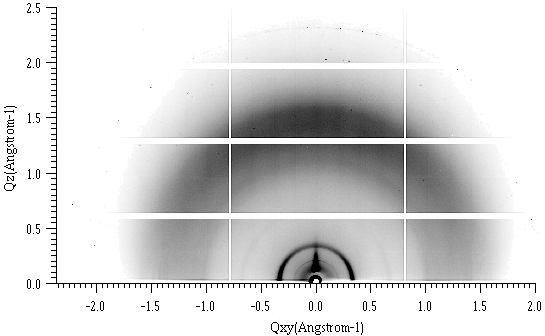
\includegraphics[width=0.8\textwidth]{ig2-8-xrd2d-cast-ch2cl2.png}
\caption{Bidimensional X-ray diffraction of \cmpd+{ig2-8} cast from \ch{CH2Cl2}.}
\label{fig:ig2-8-xrd2d-cast-ch2cl2}
\end{figure}

The thin film of \cmpd+{ig2-8} cast from \ch{CH2Cl2} was analyzed also in \gls{XRD2D} and the resulting image is reported in Figure~\ref{fig:ig2-8-xrd2d-cast-ch2cl2}. The presence of arcs indicates the absence of orientation on quartz substrate. 

Solid \cmpd+{ig2-8} was analyzed also using \gls{SAXS} and no long range spacing was observed. This information is contrary to the hypothesis of chirality originating from a large supramolecular assembly made of tilted lamellae in crystalline solid.\superfootcite{Goto2002} This is in accordance with the absence of vibronic bands in \gls{CD} spectra that should be present if the chirality rises from well ordered structures. We don't exclude the presence of a chiral supramolecular organization without ordered repetition in amorphous domains. 

\end{subsection}
\clearpage
\begin{subsection}{Photovoltaic Device Tests}
\label{cella}

\cmpd+{ig2-8} was tested in solar cells in blend with \acrfull{PCBM} nanoparticles by the Centre for Hybrid and Organic Solar
Energy (\textsmaller{CHOSE}) of the University of Rome Tor Vergata. Preliminary results are reported here, tests on \cmpd+{ig2-15} are in course. 

\begin{figure}[tbp]%ig2-11-pcbm-uvvis
\begin{tikzpicture}
\begin{axis}[axis x line=bottom,axis y line=left,enlarge x limits=false,enlarge y limits=false,width=1\textwidth,height=6cm,xlabel=Wavelength (nm),ylabel=Absorbance,legend pos=north east,cycle list name=linestyles*]
\addplot table {img/results/ig2-11-pcbm-uvvis-500rpm.txt};
\addlegendentry{\SI{500}{\rpm} (\SI{65}{\nm})};
\addplot table {img/results/ig2-11-pcbm-uvvis-1000rpm.txt};
\addlegendentry{\SI{1000}{\rpm} (\SI{55}{\nm})};
\addplot table {img/results/ig2-11-pcbm-uvvis-1500rpm.txt};
\addlegendentry{\SI{1500}{\rpm} (\SI{45}{\nm})};
\end{axis}
\end{tikzpicture} \caption[UV-vis spectra of thin films from spin coating of \cmpd+{ig2-8}:PCBM blend.]{\Gls{UVvis} spectra of thin films from spin coating of \cmpd+{ig2-8}:\gls{PCBM} blend at various rotation speeds (and film thickness). Spinning duration \SI{120}{\s}. Support soda-lime glass.}
\label{fig:ig2-11-pcbm-uvvis}
\end{figure}

The polymer was dissolved in ortho-di\-chloro\-benzene (1~\% weight) with \gls{PCBM} in a 1:1 ratio. 
This solution was used for producing thin films via spin coating. The rotation speed was varied (\SI{500}{\rpm}, \SI{1000}{\rpm} and \SI{1500}{\rpm}) in order to obtain different film thicknesses. 
\Gls{UVvis} absorption spectra (and thickness) of the obtained thin films are reported in Figure~\ref{fig:ig2-11-pcbm-uvvis}. The obtained thickness were much smaller than expected, thus we utilized \SI{400}{\rpm} for the cell production, that is the lower limit needed to obtain an uniform deposition of the film via spin coating. 
We can notice an intense absorption peak at $\lambda = $ \SI{335}{\nm} due to the \gls{PCBM} absorption. The polythio\-phene absorption peak is located at \SI{455}{\nm}, thus it was somewhat blue shifted respect to our thin films from spin coating from pure \cmpd+{ig2-8}, this is a reasonable consequence of the disorder introduced with \gls{PCBM}. 

\begin{SCfigure}[][tbp]%cella
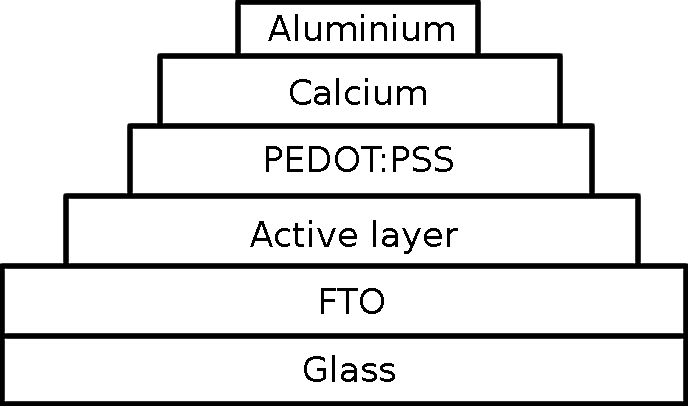
\includegraphics[width=0.4\textwidth]{cella-bn.png}
\caption{Testing cell layers scheme.}
\label{fig:cella}
\end{SCfigure}

The structure of the realized cells is reported in Figure~\ref{fig:cella}. 
The utilized architecture was the direct one, that is: \gls{FTO}\-/\acrshort{PEDOT:PSS} (\SI{50}{\nm})\-/active layer\-/\ch{Ca} (\SI{20}{\nm})\-/\ch{Al} (\SI{100}{\nm}) where \gls{FTO} is the anode and aluminium is the cathode. 
Refer to experimental section for cell preparation procedure. 
Eight cells were produced and a mean of the results is reported here. 
\gls{P3HT}:\gls{PCBM} was used in the active layer for reference cells. These reference cells were annealed at \SI{150}{\celsius} for \SI{10}{\minute} while the \cmpd+{ig2-8} based cells weren't annealed. 

\begin{table}[tbp]%pv
\centering
\caption[Characteristic parameters of solar cells from polymer-PCBM blends.]{Characteristic parameters of solar cells from polymer-\gls{PCBM} blends.}\label{tab:pv}
\begin{tabular}{c|c|c|c|c}
\toprule
polymer&$V_{oc}$ (\SI{}{\mV})&$J_{sc}$ (\SI{}{\mA\per\square\cm})&FF (\%)&$\eta$ (\%) \\ \cmidrule{1-5}
\gls{P3HT}&$0.567 \pm 0.007$&$-10.8 \pm 0.7$&$50 \pm 20$	& $3 \pm 1$ \\ 
\cmpd+{ig2-8}&$0.68 \pm 0.05$&$-3.2 \pm 0.5$&$31 \pm 3$&$0.7 \pm 0.1$\\ 
\bottomrule
\end{tabular}
\end{table}

From results in Table~\ref{tab:pv} we notice that \cmpd+{ig2-8}:\gls{PCBM} cells under illumination showed an open circuit voltage $V_{oc}$ of \SI{0.68}{\mV}, higher than that of \gls{P3HT} (\SI{0.57}{\mV}). This value is in accordance with \citeauthor*{Zoombelt2008}\superfootcite{Zoombelt2008} where a similar, but non branched, polythio\-phene side group was used. 
This is caused by the electron withdrawing effect of the oxy\-gen atom in side chain respect to the methylene in \gls{P3HT}. The measured short circuit current density $J_{sc}$ from \cmpd+{ig2-8} was lower than the current from \gls{P3HT}. We think that this is caused by worse crystallization due the presence of branching in side group and by the presence of the oxy\-gen atom, as reported by \citeauthor*{Zoombelt2008}.\superfootcite{Zoombelt2008} 
The obtained \gls{FF} was rather low (31~\%) and the resulting power conversion efficiency $\eta$ resulted 0.7~\% versus and efficiency of 
3~\% from the reference cells. 
Considering the high $V_{oc}$ observed this is a promising candidate for block copolymer synthesis and its use in bulk heterojunction solar cells active layer. 

\end{subsection}
\end{section}
\clearpage
\begin{section}{Second Block}

Two main approaches are common in the synthesis of diblock copolymers: grafting onto, which means joining two blocks after their polymerization, and grafting from, which means starting the polymerization of the second block from a termination of the first block. The grafting onto way allows one to polymerize both blocks in a clean reaction environment and permits a better characterization of the single blocks prior to coupling. 
But in the present case the grafting onto approach is hampered by the chelating behavior of the \gls{P4VP} block that would interfere with the joining reaction. 
Thus a grafting from approach was followed, polymerizing the \gls{P4VP} block starting from an adequately functionalized end of \cmpd+{ig2-8}. 
Two poly\-thio\-phene-\textit{block}-poly\-vinyl\-pyridine syntheses were already present in the literature. \Citeauthor*{Lohwasser2012}\superfootcite{Lohwasser2012} synthesized an alkyne-terminated poly\-thio\-phene, then, using a click reaction, they functionalized the alkyne termination with an initiator for poly\-vinyl\-pyridine polymerization. 
We decided to don't follow this route because the formation of the alkyne end capper is reported to produce both mono and di terminated poly\-thio\-phene chains.\superfootcite{Jeffries-EL2004}\superfootcite{Jeffries-El2005} Moreover the triple bond is sensible to the standard quenching procedure and there are questions on the efficiency of the click reaction on a triple bond conjugated to a poly\-thio\-phene chain.\superfootcite{Urien2008} 
\Citeauthor*{Sary2010a}\superfootcite{Sary2010a} synthesized an \ch{H/Br} terminated poly\-thio\-phene, then they employed the halogenated termination to functionalize the polymer with an aldehyde group. Then the polythio\-phene-aldehyde was used as a quenching agent for vinyl\-pyridine anionic polymerization. This route was discarded because of the strict reaction conditions needed by an anionic polymerization.

For the synthesis of the first polythio\-phenic block we followed polymerization methods which were reported producing high yields in \ch{H/Br} terminated chains. 
Then we tried to functionalize the halogenated endings of our polymers with a boronic ester. We reacted \cmpd+{ig2-8} with \textit{n}-butyl\-lithium in \gls{THF} at low temperature, then we added 2-iso\-prop\-oxy-4,4,5,5-tetra\-methyl-1,3,2-di\-oxa\-borolane in order to produce a pinacol ester of the poly\-thio\-phene boronic acid. Although trying thrice this functionalization with different \textit{n}-butyl\-lithium quantities, we didn't get the boron atom bonded to the polymer (this was confirmed by \gls{FTIR}, {\HNMR} and {\CNMR} spectroscopies and later by \gls{MALDI}). 

So we followed a procedure similar to the strategy from \citeauthor*{Sary2010a}\superfootcite{Sary2010a} but avoiding the anionic polymerization. In the first step we functionalized the polymer \cmpd+{ig2-8} on the halogenated sites using a Suzuki coupling. The functionalizing group was chosen as a di\-thio\-phene bearing a boronic acid group and a formyl group. We preferred using a thio\-phenic end capper because the similarity of its electronic levels to the levels of the rest of the chain should avoid the possible charge trapping on the end capper. Then this aldehyde-terminated chiral poly\-thio\-phene was reacted with the lithium activated polymerization initiator. Finally a poly\-(4-vinyl\-pyridine) block was polymerized starting from this group. 

\begin{subsection}{Radical Mediator Synthesis and Characterization}
The polymerization of \gls{P4VP} was a living radical polymerization mediated by the \gls{TIPNO} radical.\superfootcite{Lohmeijer2005} This radical is a commercial product but we need to build an initiator molecule (containing the radical) suitable to be attached on a poly\-thio\-phene end. We synthesized \gls{BrPhEtTIPNO} \cmpd+{ig2-21} which will be lithiated on the bromine atom for the linking to an aldehyde-terminated poly\-thio\-phene. 

\begin{figure}[tbp]%syn-tipno
\centering
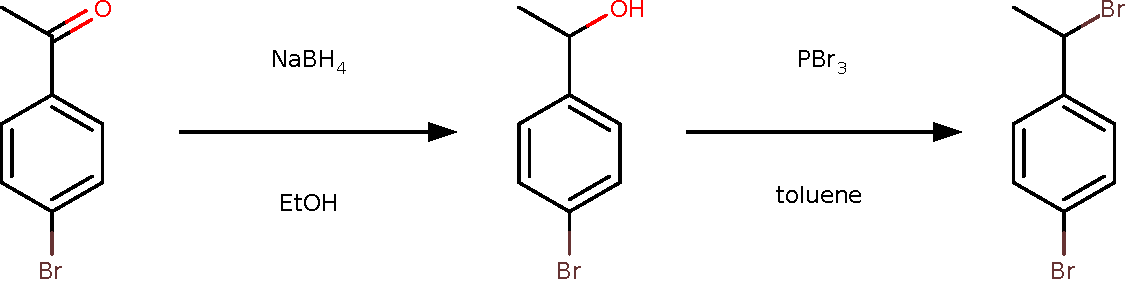
\includegraphics[scale=0.7]
{syn6-7-riduzione-bromurazione.pdf}
\medskip
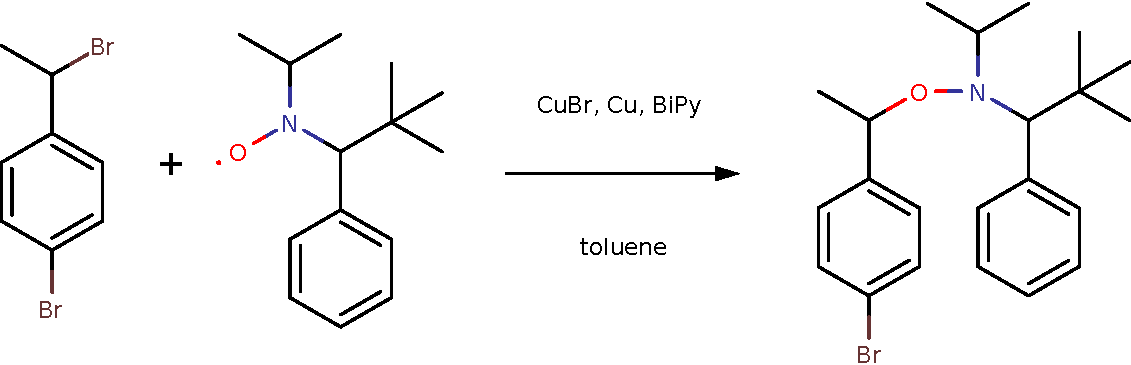
\includegraphics[scale=0.7]
{syn8-tipno-br.pdf} 
\caption[PhEt-TIPNO synthesis.]{\Acrfull{BrPhEtTIPNO} \cmpd+{ig2-21} synthesis.}
\label{fig:syn-tipno}
\end{figure}

As shown in Figure~\ref{fig:syn-tipno} we started reducing 4-bromo\-aceto\-phenone to 1-(4-bromo\-phenyl)\-ethanol \cmpd+{ig2-16} via a simple reaction with sodium boro\-hydride.\superfootcite{Wiles2006} Then we brominated\superfootcite{Stalmach2001} 1-(4-bromo\-phenyl)\-ethanol \cmpd+{ig2-16} with phosphorus tri\-bromide (\ch{PBr3}) obtaining a mixture of 1-bromo-4-(1-bromo\-ethyl)\-benzene \cmpd+{ig2-17} and 4-bromo\-styrene. This mixture was reacted with \gls{TIPNO} radical in a copper(I) catalyzed coupling.\superfootcite{Benoit1999} The purification was carried on basic allumina (in order to avoid the evenience of a breaking of the nitr\-oxyde group on the slightly acid silica). 

The resulting product was characterized with poor results using \gls{GCMS} with a modified on purpose method (injector and transfer line temperatures were lowered), then the structure was confirmed by {\HNMR}, the assignation is reported in experimental section and the spectra is reported in appendix.

\end{subsection}
\begin{subsection}{Functionalization of Polythio\-phene with Radical Mediator}
\begin{figure}[tbp]%syn9-suzuki
\centering
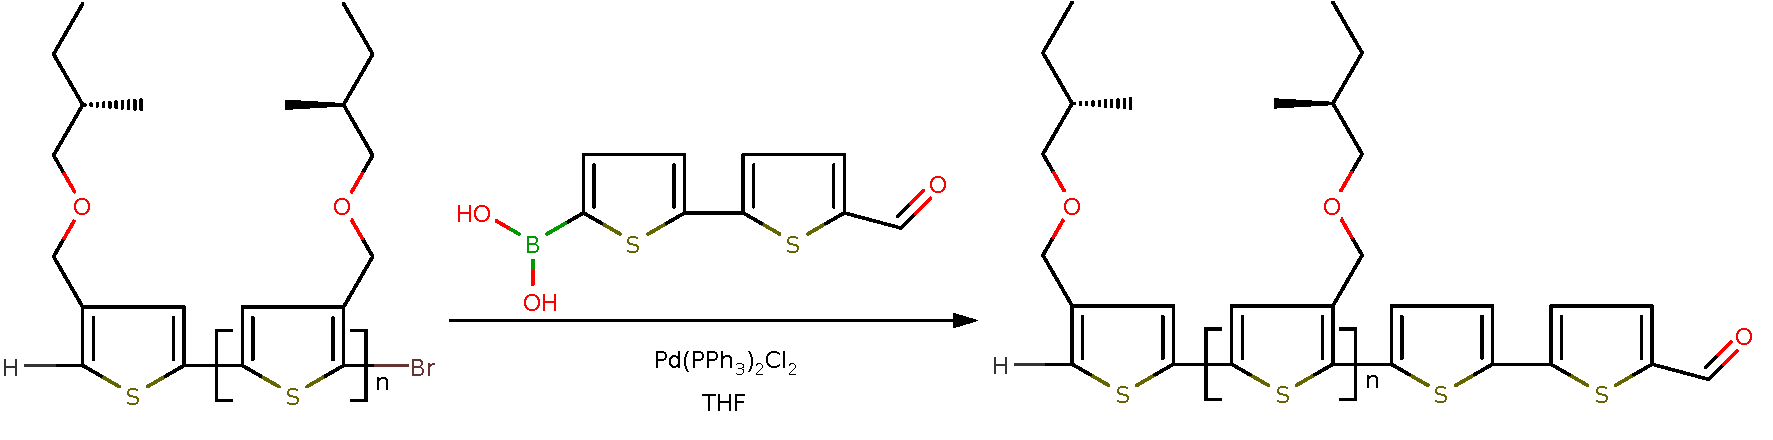
\includegraphics[width=1\textwidth]
{syn9-suzuki.pdf}
\caption{End-functionalization of poly\-thio\-phene with aldehyde using a Suzuki reaction.}
\label{fig:syn9-suzuki}
\end{figure}

The poly\-thio\-phene \cmpd+{ig2-8} was functionalized with an aldehyde group via palladium catalyzed Suzuki coupling with B-(5'-formyl\-[2,2'-bi\-thio\-phen]\-5-yl)\-boronic acid, as schematized in Figure~\ref{fig:syn9-suzuki}. We followed a procedure reported in literature\superfootcite{Zhang2011}\superfootcite{Imae2012} but with a significant variation: we substituted the tetra\-kis\-(tri\-phenyl\-phosphine)\-palladium(0) (\ch{Pd(PPh3)4}) catalyst with the more stable bis\-(tri\-phenyl\-phosphine)\-palladium(II) di\-chloride (\ch{Pd(PPh3)2Cl2}). We found (in a test reaction involving a low molecular weight halogenated thio\-phene) that this convenient catalyst works for our coupling. 
The functionalized polymer \cmpd+{ig2-19} was purified via precipitation, washing and redissolved in various solvents. The presence of an aldehyde group was confirmed by \gls{FTIR} spectroscopy and {\HNMR} (in \gls{TCE}-d$_2$) by the appearance of a peak at \SI{9.80}{\ppm} attributable to carbonylic proton. 

Then the \gls{BrPhEtTIPNO} \cmpd+{ig2-21} was lithiated with one equivalent of \textit{n}-buthyl\-lithium in \gls{THF} and poured in well dissolved (in \gls{THF} at \SI{50}{\celsius}) poly\-thio\-phene-aldehyde \cmpd+{ig2-19} obtaining the macroinitiator poly\-thio\-phene-\gls{TIPNO} \cmpd+{ig2-22}. The reaction yield was estimated from the decrease of the aldehyde peak in {\HNMR} spectrum and resulted $\approx90$~\% (see spectra in appendix, also new peaks in aromatic region can be noticed). The lithiation completeness was verified by quenching with water an aliquot of lithium activated \gls{BrPhEtTIPNO}, the \gls{GCMS} analysis showed the absence of brominated compounds.

\begin{figure}[tbp]%syn10-pt-tipno
\centering
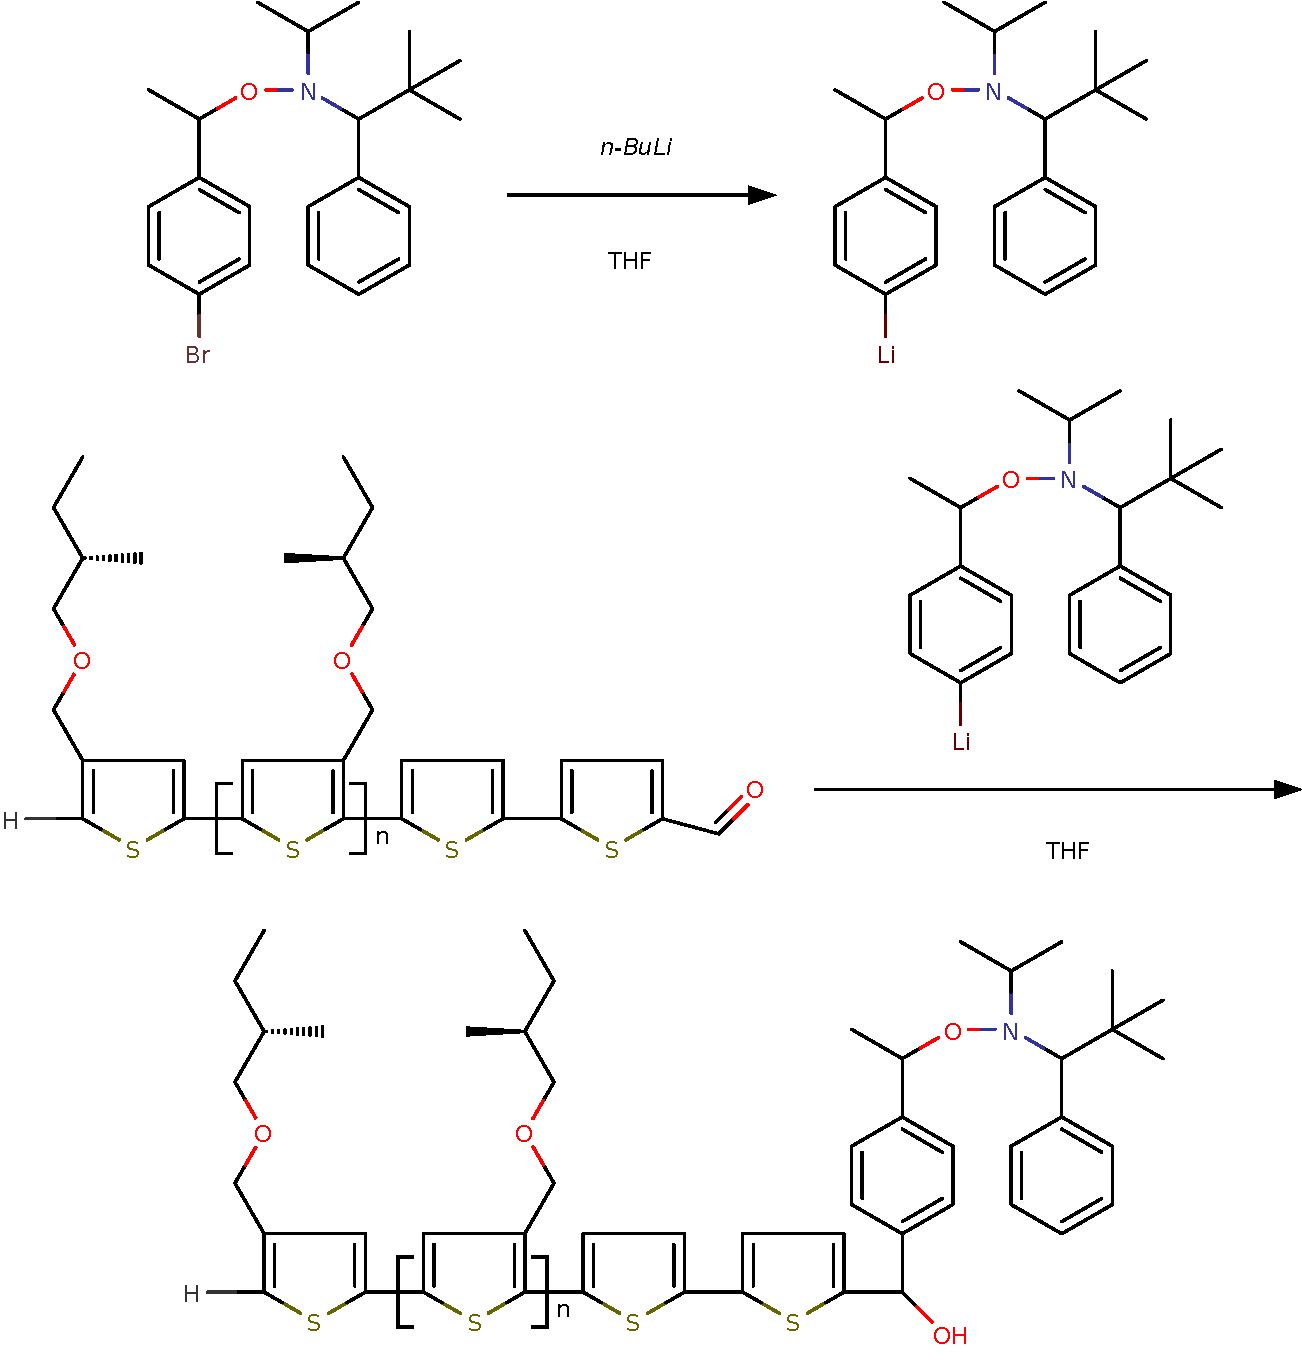
\includegraphics[scale=0.5]
{syn10-pt-tipno.pdf}
\caption[Functionalization of poly\-thio\-phene-aldehyde \cmpd+{ig2-19} with PhEt-TIPNO \cmpd+{ig2-21} obtaining the macroinitiator \cmpd+{ig2-22}.]{Functionalization of poly\-thio\-phene-aldehyde \cmpd+{ig2-19} with \gls{BrPhEtTIPNO} \cmpd+{ig2-21} obtaining the macroinitiator \cmpd+{ig2-22}.}
\label{fig:syn10-pt-tipno}
\end{figure}

\end{subsection}
\begin{subsection}{Second Block Synthesis and Characterization}
\label{sec:nmrp}

\begin{figure}[tbp]%syn11-p4vp
\centering
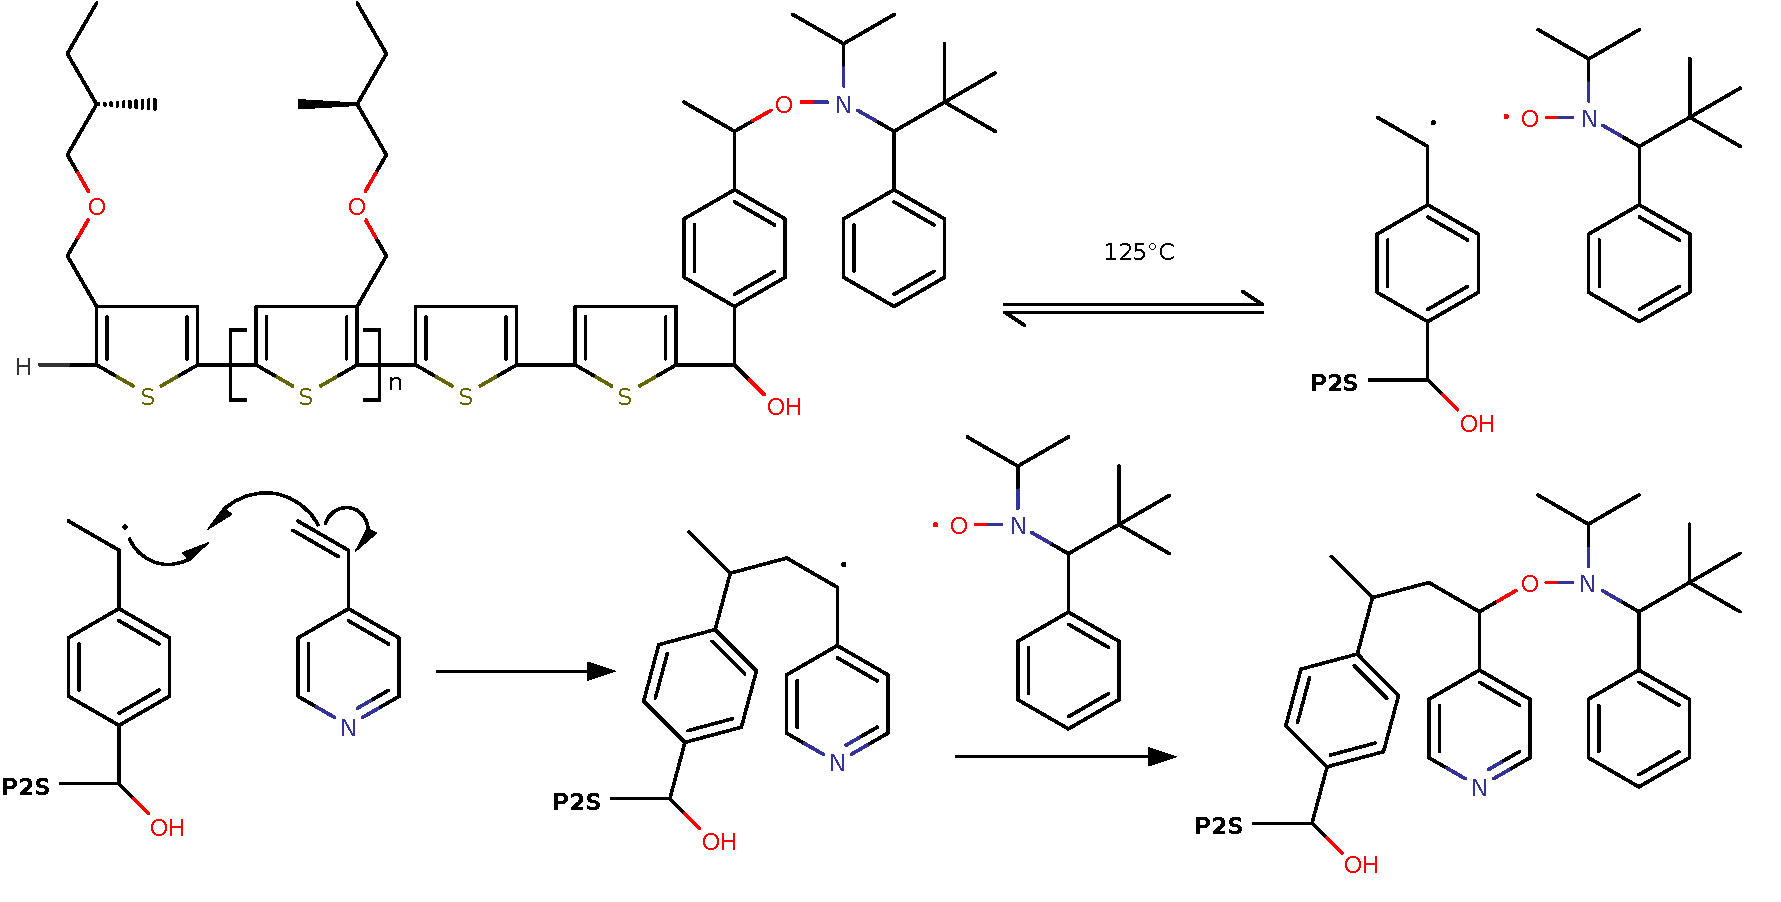
\includegraphics[width=1\textwidth]
{syn11-p4vp.pdf}
\caption[NMRP polymerization of P4VP starting from macroinitiator \cmpd+{ig2-22} and obtaining block copolymer \cmpd+{sz17}.]{\gls{NMRP} polymerization of \gls{P4VP} starting from macroinitiator \cmpd+{ig2-22} and obtaining block copolymer \cmpd+{sz17}.}
\label{fig:syn11-p4vp}
\end{figure}

\Acrfull{NMRP} polymerization of vinyl\-pyridine was performed following procedure from \citeauthor*{Lohwasser2012}.\superfootcite{Lohwasser2012} The radical polymerization was initiated by heating at \SI{125}{\celsius} the solution of macroinitiator \cmpd+{ig2-22} in ortho-di\-chloro\-benzene containing 4-vinyl\-pyridine in a molar ratio of 1:3000 with addition of free radical \gls{TIPNO} (enhances the control on the polymerization). The polymerization was run for \SI{4}{\hour}. The molar ratio and the duration were modified with respect to the reference article in order to reduce the formation of \gls{P4VP} homo\-polymer. Then the reaction was cooled down, diluted in chloroform and poured in hexane. 
Hexane is a poor solvent for both poly\-thio\-phene and poly\-vinyl\-pyridine, thus the solid was filtered and recovered in chloroform, that is a good solvent for both blocks. The chloroform solution was poured again in methanol, that is a good solvent only for poly\-vinyl\-pyridine block. {\HNMR} characterization of this methanol fraction showed the presence of vinyl\-pyridine homo\-polymers and small molecules, no peaks for thio\-phenic units. 
The solid was filtered and washed with hot toluene (\SI{70}{\celsius}) that is a good solvent (at room temperature is poor) for the poly\-thio\-phene block only. With {\HNMR} we verified the absence of poly\-vinyl\-pyridine aromatic peaks looking both for aromatic and aliphatic protons (spectra with expansions in appendix). The remaining solid was recovered in chloroform obtaining the block copolymer \cmpd+{sz17}. {\HNMR} analysis on this fraction, reported in Figure~\ref{fig:sz17-nmr-h-zoom-py}, showed the presence of broad aromatic (\SI{8.26}{\ppm} and \SI{6.35}{\ppm} in \gls{TCE}-d$_2$) and aliphatic (\SI{0.83}{\ppm} and \SI{0.79}{\ppm} in \gls{TCE}-d$_2$) peaks assigned to a short block of poly\-vinyl\-pyridine together with the usual peaks from poly\-thio\-phene block. 
Comparing with \gls{NMR} spectrum from \cmpd+{ig2-22} we can notice also variations in peaks around \SI{7.4}{\ppm} that are related to the \gls{TIPNO} group. A confirmation of the removal of unreacted thio\-phenic homo\-polymer come from an aldehydic {\HNMR} peak: The impurities of unreacted polythio\-phene-aldehyde \cmpd+{ig2-19} (in the functionalization reaction with lithiated \gls{BrPhEtTIPNO} \cmpd+{ig2-21}) can't work as a macroinitiator for a \gls{P4VP} block, the fact that in the toluene fraction we can see an aldehyde \gls{NMR} peak at \SI{9.80}{\ppm} that is 5 times more intense than the corresponding peak in the purified fraction means that the majority of homo\-polymer was washed in hot toluene. 

The purification procedure reported by the reference article\superfootcite{Lohwasser2012} was more complex and not suitable for small quantities (we worked with less than \SI{20}{\mg} of product). 
Indeed our simpler purification method 
was effective. The relative quantity of pyridine rings can be estimated by integration of aromatic protons, from this calculation results that for every pyridine ring there are 5 thio\-phene rings, thus around 10 pyridine rings per polythio\-phene chain. The length of this block is inferior to that reported from similar syntheses.\superfootcite{Lohwasser2012}\superfootcite{Mougnier2012}

\begin{figure}[tbp]%sz17-nmr-h-zoom-py
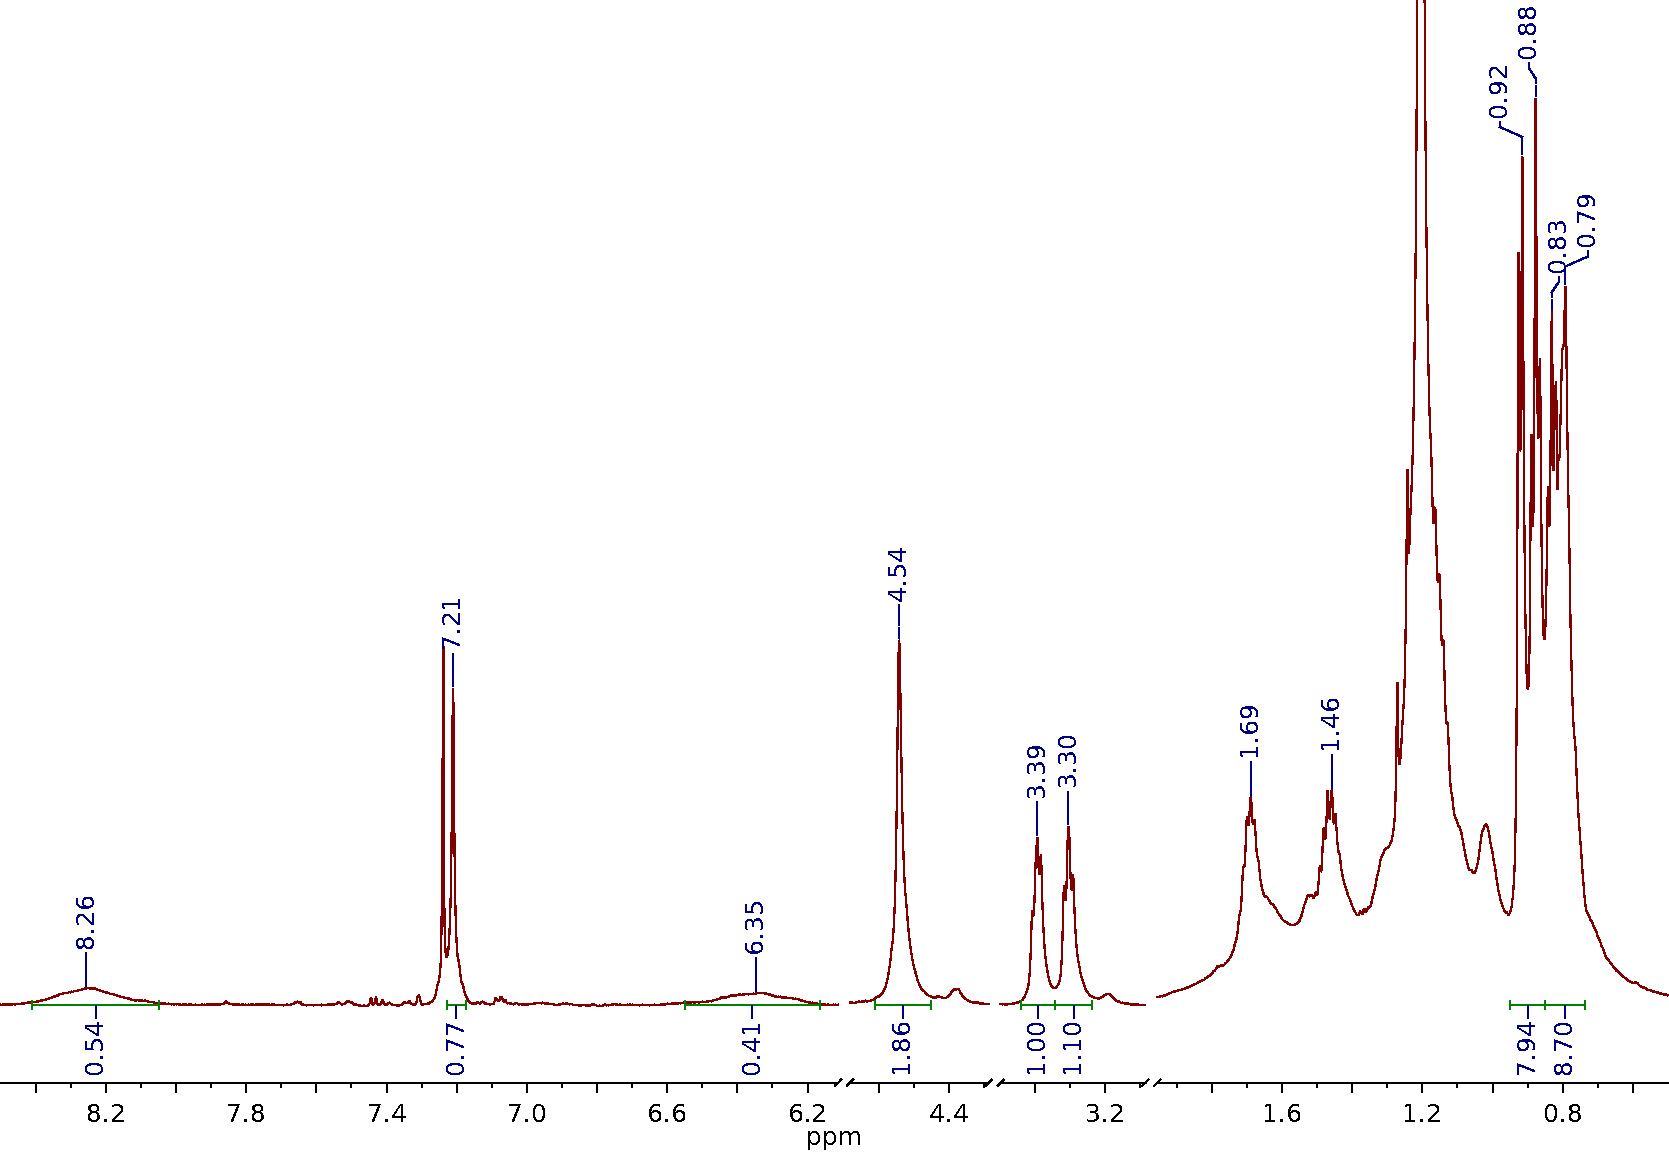
\includegraphics[width=0.99\textwidth]{sz17-nmr-h-zoom-py.pdf}
\caption[{\HNMR} of poly\-thio\-phene-poly\-vinyl\-pyridine \cmpd+{sz17}.]{{\HNMR} (\SI{600}{\MHz}) of poly\-thio\-phene-poly\-vinyl\-pyridine \cmpd+{sz17} in \gls{TCE}-d2.}
\label{fig:sz17-nmr-h-zoom-py}
\end{figure}

Preliminary optical characterizations were performed on the new di\-block copolymer \cmpd+{sz17}. \Gls{UVvis} spectroscopy in chloroform showed a spectra similar to \cmpd+{ig2-8} but the intensity was halved, maybe due the presence of \gls{P4VP} (or due to non proper drying). 
Adding 40~\% methanol to a chloroform solution resulted in a \SI{12}{\nm} red shift in main \gls{UVvis} peak, related to a polythio\-phene $\pi-\pi^*$ transition. With additional 10~\% of methanol resulted in a further red shift of \SI{10}{\nm} (see data in Table~\ref{tab:sz17-cd}). We don't observe the usual quenching of the peak at \SI{260}{\nm} because in that region there's also the main absorption peak of pyridine. 

\begin{table}%sz17-cd
\centering
\caption[UV-vis and CD data of \cmpd+{sz17} solutions.]{\gls{UVvis} and \gls{CD} data of \cmpd+{sz17} solutions. Concentration \SI{137}{\mg\per\liter}. Pathlength \SI{1}{\mm}.}\label{tab:sz17-cd}
\begin{tabular}{c|c|c|c}
\toprule
processing&\tallcell{UV-vis\\ peak\\(\SI{}{nm})}&\tallcell{CD\\ inflection\\(\SI{}{nm})}&\tallcell{CD\\ amplitude\\(\SI{}{mdeg})}\\ \cmidrule{1-4}
\ch{CHCl3} solution 				&440&&\\
\ch{CHCl3} 80 \% - \ch{MeOH} 20 \%	&438&&\\
\ch{CHCl3} 70 \% - \ch{MeOH} 30 \%	&440&&\\
\ch{CHCl3} 70 \% - \ch{MeOH} 30 \% \SI{1}{\day}&440&$\approx448$&0.36\\
\ch{CHCl3} 60 \% - \ch{MeOH} 40 \%	&452&464&1.4\\
\ch{CHCl3} 50 \% - \ch{MeOH} 50 \%	&462&461&3.2\\
\ch{CHCl3} 30 \% - \ch{MeOH} 70 \%	&464&460&4.7\\

\bottomrule
\end{tabular}
\end{table}

\begin{figure}[tbp]%sz17-uvvis
\begin{tikzpicture}
\begin{axis}[axis x line=bottom,axis y line=left,enlarge x limits=false,enlarge y limits=false,width=1\textwidth,height=8cm,xlabel=Wavelength (nm),ylabel=Absorbance,xmin=240,xmax=650,legend style={at={(0.05,1.1)},anchor=north west,font=\footnotesize},cycle list name=linestyles*]
\addplot table {img/results/sz17-uvvis-137-chcl3-70-meoh-30.txt};
\addlegendentry{in \ch{CHCl3} 70 \% - \ch{MeOH} 30 \%};
\addplot table {img/results/sz17-uvvis-137-chcl3-60-meoh-40.txt};
\addlegendentry{in \ch{CHCl3} 60 \% - \ch{MeOH} 40 \%};
\addplot table {img/results/sz17-uvvis-137-chcl3-50-meoh-50.txt};
\addlegendentry{in \ch{CHCl3} 50 \% - \ch{MeOH} 50 \%};
\addplot table {img/results/sz17-uvvis-137-chcl3-30-meoh-70.txt};
\addlegendentry{in \ch{CHCl3} 30 \% - \ch{MeOH} 70 \%};
\end{axis}
\end{tikzpicture} \caption[UV-vis spectra of block copolymer \cmpd+{sz17} in mixtures of good-poor solvent.]{UV-vis spectra of polymer \cmpd+{sz17} in chloroform-methanol mixtures. Concentration \SI{137}{\mg\per\liter}. Pathlength \SI{1}{\mm}.}
\label{fig:sz17-uvvis}
\end{figure}

Comparing \gls{CD} spectra in chloroform-methanol solutions of \cmpd+{sz17} with spectra from \cmpd+{ig2-8} we can observe some differences. With \cmpd+{ig2-8}, up to 30~\% of methanol no \gls{CD} signal can be observed but waiting one day, \cmpd+{ig2-8} in 30~\% of methanol showed a very intense bisignate couplet (see Figure~\ref{fig:ig2-8-cd-meoh-1}) while \cmpd+{sz17} showed only an extremely weak signal in the same conditions. 
Adding more methanol resulted in an increase of the \gls{CD} intensity. Comparing intensities of \gls{CD} spectra of \cmpd+{sz17} and \cmpd+{ig2-8} in similar concentrations of methanol, \cmpd+{sz17} showed an optical activity around 6 times weaker. 
These differences should be related to the \gls{P4VP} block that is soluble both in chloroform and in methanol and could help the polythio\-phene block to remain in solution or could interfere with its supramolecular organization. We hypothesize the formation of direct micelles. 

\begin{figure}[tbp]%sz17-cd
\begin{tikzpicture}
\begin{axis}[axis x line=bottom,axis y line=left,enlarge x limits=false,enlarge y limits=true,width=1\textwidth,height=8cm,xlabel=Wavelength (nm),ylabel=Circular Dichroism (mdeg),xmin=240,xmax=600,legend pos=north west,cycle list name=linestyles*]
\addplot table {img/results/sz17-cd-137-chcl3-70-meoh-30-1day.txt};
\addlegendentry{in \ch{CHCl3} 70 \% - \ch{MeOH} 30 \% \SI{1}{\day}};
\addplot table {img/results/sz17-cd-137-chcl3-60-meoh-40.txt};
\addlegendentry{in \ch{CHCl3} 60 \% - \ch{MeOH} 40 \%};
\addplot table {img/results/sz17-cd-137-chcl3-50-meoh-50.txt};
\addlegendentry{in \ch{CHCl3} 50 \% - \ch{MeOH} 50 \%};
\addplot table {img/results/sz17-cd-137-chcl3-30-meoh-70.txt};
\addlegendentry{in \ch{CHCl3} 30 \% - \ch{MeOH} 70 \%};
\draw[help lines] (axis cs:240,0) -- (axis cs:600,0);
\end{axis}
\end{tikzpicture} \caption{Circular dichroism spectra of block copolymer \cmpd+{sz17} in chloroform-methanol solvent mixtures. Concentration \SI{137}{\mg\per\liter}. Pathlength \SI{1}{\mm}.}
\label{fig:sz17-cd}
\end{figure}

\end{subsection}
\end{section} 
